% Options for packages loaded elsewhere
\PassOptionsToPackage{unicode}{hyperref}
\PassOptionsToPackage{hyphens}{url}
%
\documentclass[
  8pt,
  ignorenonframetext,
]{beamer}
\usepackage{pgfpages}
\setbeamertemplate{caption}[numbered]
\setbeamertemplate{caption label separator}{: }
\setbeamercolor{caption name}{fg=normal text.fg}
\beamertemplatenavigationsymbolsempty
% Prevent slide breaks in the middle of a paragraph
\widowpenalties 1 10000
\raggedbottom
\setbeamertemplate{part page}{
  \centering
  \begin{beamercolorbox}[sep=16pt,center]{part title}
    \usebeamerfont{part title}\insertpart\par
  \end{beamercolorbox}
}
\setbeamertemplate{section page}{
  \centering
  \begin{beamercolorbox}[sep=12pt,center]{part title}
    \usebeamerfont{section title}\insertsection\par
  \end{beamercolorbox}
}
\setbeamertemplate{subsection page}{
  \centering
  \begin{beamercolorbox}[sep=8pt,center]{part title}
    \usebeamerfont{subsection title}\insertsubsection\par
  \end{beamercolorbox}
}
\AtBeginPart{
  \frame{\partpage}
}
\AtBeginSection{
  \ifbibliography
  \else
    \frame{\sectionpage}
  \fi
}
\AtBeginSubsection{
  \frame{\subsectionpage}
}
\usepackage{amsmath,amssymb}
\usepackage{lmodern}
\usepackage{ifxetex,ifluatex}
\ifnum 0\ifxetex 1\fi\ifluatex 1\fi=0 % if pdftex
  \usepackage[T1]{fontenc}
  \usepackage[utf8]{inputenc}
  \usepackage{textcomp} % provide euro and other symbols
\else % if luatex or xetex
  \usepackage{unicode-math}
  \defaultfontfeatures{Scale=MatchLowercase}
  \defaultfontfeatures[\rmfamily]{Ligatures=TeX,Scale=1}
\fi
% Use upquote if available, for straight quotes in verbatim environments
\IfFileExists{upquote.sty}{\usepackage{upquote}}{}
\IfFileExists{microtype.sty}{% use microtype if available
  \usepackage[]{microtype}
  \UseMicrotypeSet[protrusion]{basicmath} % disable protrusion for tt fonts
}{}
\makeatletter
\@ifundefined{KOMAClassName}{% if non-KOMA class
  \IfFileExists{parskip.sty}{%
    \usepackage{parskip}
  }{% else
    \setlength{\parindent}{0pt}
    \setlength{\parskip}{6pt plus 2pt minus 1pt}}
}{% if KOMA class
  \KOMAoptions{parskip=half}}
\makeatother
\usepackage{xcolor}
\IfFileExists{xurl.sty}{\usepackage{xurl}}{} % add URL line breaks if available
\IfFileExists{bookmark.sty}{\usepackage{bookmark}}{\usepackage{hyperref}}
\hypersetup{
  hidelinks,
  pdfcreator={LaTeX via pandoc}}
\urlstyle{same} % disable monospaced font for URLs
\newif\ifbibliography
\usepackage{longtable,booktabs,array}
\usepackage{calc} % for calculating minipage widths
\usepackage{caption}
% Make caption package work with longtable
\makeatletter
\def\fnum@table{\tablename~\thetable}
\makeatother
\setlength{\emergencystretch}{3em} % prevent overfull lines
\providecommand{\tightlist}{%
  \setlength{\itemsep}{0pt}\setlength{\parskip}{0pt}}
\setcounter{secnumdepth}{-\maxdimen} % remove section numbering
% type setting
% ------------------------------------------------------------------------------
\usepackage[german]{babel}     

% fonts
% ------------------------------------------------------------------------------
\usefonttheme{professionalfonts}

% slide title and horizontal line
% ------------------------------------------------------------------------------
\setbeamertemplate{frametitle}{%
    \vskip-30pt \color{black}\large%
    \begin{minipage}[b][23pt]{120mm}%
    \flushleft\insertframetitle%
    \end{minipage}%
}

\setbeamertemplate{headline}										
{
\vskip10pt\hfill\hspace{3.5mm} 										 
\vskip15pt\color{black}\rule{\textwidth}{0.4pt} 					 
}

% slide number
% ---------------------------------------------------------------
\setbeamertemplate{navigation symbols}{}
\setbeamertemplate{footline}
{
\vskip5pt
\vskip2pt
\makebox[123mm]{\hspace{7.5mm}
\hfill Allgemeines Lineares Modell $\vert$ 
\copyright $ $ 2022 Dirk Ostwald CC BY-NC-SA 4.0 $\vert$ 
Folie \insertframenumber}
\vskip4pt
}

% block color scheme
% ------------------------------------------------------------------------------
% colors
\definecolor{white}{RGB}{255,255,255}
\definecolor{grey}{RGB}{235,235,235}
\definecolor{lightgrey}{RGB}{245,245,245}
\definecolor{LightBlue}{RGB}{220,220,255}
\definecolor{darkblue}{RGB}{51, 51, 153}

% definitions and theorems
\setbeamercolor{block title}{fg = black, bg = grey}
\setbeamercolor{block body}{fg = black, bg = lightgrey}

% general line spacing 
% ------------------------------------------------------------------------------
\linespread{1.3}

% local line spacing
% ------------------------------------------------------------------------------
\usepackage{setspace}

% colors
% -----------------------------------------------------------------------------
\usepackage{color}

% justified text
% ------------------------------------------------------------------------------
\usepackage{ragged2e}
\usepackage{etoolbox}
\apptocmd{\frame}{}{\justifying}{}

% bullet point lists
% -----------------------------------------------------------------------------
\setbeamertemplate{itemize item}[circle]
\setbeamertemplate{itemize subitem}[circle]
\setbeamertemplate{itemize subsubitem}[circle]
\setbeamercolor{itemize item}{fg = black}
\setbeamercolor{itemize subitem}{fg = black}
\setbeamercolor{itemize subsubitem}{fg = black}
\setbeamercolor{enumerate item}{fg = black}
\setbeamercolor{enumerate subitem}{fg = black}
\setbeamercolor{enumerate subsubitem}{fg = black}
\setbeamerfont{itemize/enumerate body}{}
\setbeamerfont{itemize/enumerate subbody}{size = \normalsize}
\setbeamerfont{itemize/enumerate subsubbody}{size = \normalsize}

% color links
% ------------------------------------------------------------------------------
\usepackage{hyperref}
\definecolor{urls}{RGB}{204,0,0}
\hypersetup{colorlinks, citecolor = darkblue, urlcolor = urls}


% additional math commands
% ------------------------------------------------------------------------------
\usepackage{bm}     
\newcommand{\niton}{\not\owns}
\DeclareMathOperator*{\intinf}{\int_{-\infty}^{\infty}}
\DeclareSymbolFont{extraitalic}      {U}{zavm}{m}{it}
\DeclareMathSymbol{\Qoppa}{\mathord}{extraitalic}{161}
\DeclareMathSymbol{\qoppa}{\mathord}{extraitalic}{162}

% text highlighting
% ------------------------------------------------------------------------------
\usepackage{soul}
\makeatletter
\let\HL\hl
\renewcommand\hl{%
  \let\set@color\beamerorig@set@color
  \let\reset@color\beamerorig@reset@color
  \HL}
\makeatother

% equation highlighting
% -----------------------------------------------------------------------------
\newcommand{\highlight}[2][yellow]{\mathchoice%
  {\colorbox{#1}{$\displaystyle#2$}}%
  {\colorbox{#1}{$\textstyle#2$}}%
  {\colorbox{#1}{$\scriptstyle#2$}}%
  {\colorbox{#1}{$\scriptscriptstyle#2$}}}%

% additional mathematical operators
% ------------------------------------------------------------------------------
\DeclareMathOperator*{\argmax}{arg\,max}
\DeclareMathOperator*{\argmin}{arg\,min}

\ifluatex
  \usepackage{selnolig}  % disable illegal ligatures
\fi
\newlength{\cslhangindent}
\setlength{\cslhangindent}{1.5em}
\newlength{\csllabelwidth}
\setlength{\csllabelwidth}{3em}
\newenvironment{CSLReferences}[2] % #1 hanging-ident, #2 entry spacing
 {% don't indent paragraphs
  \setlength{\parindent}{0pt}
  % turn on hanging indent if param 1 is 1
  \ifodd #1 \everypar{\setlength{\hangindent}{\cslhangindent}}\ignorespaces\fi
  % set entry spacing
  \ifnum #2 > 0
  \setlength{\parskip}{#2\baselineskip}
  \fi
 }%
 {}
\usepackage{calc}
\newcommand{\CSLBlock}[1]{#1\hfill\break}
\newcommand{\CSLLeftMargin}[1]{\parbox[t]{\csllabelwidth}{#1}}
\newcommand{\CSLRightInline}[1]{\parbox[t]{\linewidth - \csllabelwidth}{#1}\break}
\newcommand{\CSLIndent}[1]{\hspace{\cslhangindent}#1}

\author{}
\date{\vspace{-2.5em}}

\begin{document}

\begin{frame}[plain]{}
\protect\hypertarget{section}{}
\center

\begin{center}
\includegraphics[width=0.2\linewidth]{8_Abbildungen/alm_8_otto} \end{center}

\vspace{2mm}

\huge

Allgemeines Lineares Modell \vspace{6mm}

\large

BSc Psychologie SoSe 2022

\vspace{6mm}
\normalsize

Prof.~Dr.~Dirk Ostwald
\end{frame}

\begin{frame}[plain]{}
\protect\hypertarget{section-1}{}
\center
\huge
\vfill

\noindent (8) Studiendesign \vfill
\end{frame}

\begin{frame}{Überblick}
\protect\hypertarget{uxfcberblick}{}
\small
\center
\footnotesize
\renewcommand{\arraystretch}{1.1}
\begin{tabular}{lll}
Datum        & Einheit                       & Thema                                              \\\hline
08.04.2022   & Grundlagen                    & (1) Regression                                 \\
             & \textcolor{gray}{Osterpause}                                             \\
22.04.2022   & Grundlagen                    & (2) Korrelation                            \\
29.04.2022   & Grundlagen                    & (3) Matrizen                             \\
06.05.2022   & Grundlagen                    & (4) Normalverteilungen                   \\
13.05.2022   & Theorie                       & (5) Modellformulierung                   \\
20.05.2022   & Theorie                       & (6) Modellschätzung                      \\
27.05.2022   & Theorie                       & (7) Modellevaluation                     \\
03.06.2021   & Anwendung                     & (8) Studiendesign                        \\
10.06.2021   & Anwendung                     & (9) T-Tests                              \\
17.06.2021   & Anwendung                     & (10) Einfaktorielle Varianzanalyse       \\
24.06.2022   & Anwendung                     & (11) Zweifaktorielle Varianzanalyse      \\
01.07.2022   & Anwendung                     & (12) Multiple Regression                 \\
08.07.2022   & Anwendung                     & (13) Kovarianzanalyse                    \\\hline
14.07.2022   & Klausurtermin                 &                                          \\
März 2023    & Klausurwiederholungstermin    &
\end{tabular}
\end{frame}

\begin{frame}{Überblick}
\protect\hypertarget{uxfcberblick-1}{}
\setstretch{3}

Studiendesign

\begin{itemize}
\item
  Einführung in die grundlegende Nomenklatur des Studiendesigns
\item
  Grundlegende Logik experimenteller Kontrolle durch Subtraktion
\item
  Grundlegende Logik faktorieller Studiendesigns
\item
  Anwendungsbeispiel für ALM Designs im weiteren Kursverlauf
\end{itemize}
\end{frame}

\begin{frame}[plain]{}
\protect\hypertarget{section-2}{}
\vfill
\large
\setstretch{2.5}

Grundbegriffe

Randomisierte einfaktorielle Studiendesigns

Randomisierte mehrfaktorielle Studiendesigns

Anwendungskontext

Anwendungsbeispiel

Selbstkontrollfragen \vfill
\end{frame}

\begin{frame}[plain]{}
\protect\hypertarget{section-3}{}
\vfill
\large
\setstretch{2.5}

\textbf{Grundbegriffe}

Randomisierte einfaktorielle Studiendesigns

Randomisierte mehrfaktorielle Studiendesigns

Anwendungskontext

Anwendungsbeispiel

Selbstkontrollfragen \vfill
\end{frame}

\begin{frame}{Grundbegriffe}
\protect\hypertarget{grundbegriffe}{}
\large

\textcolor{darkblue}{Empirische Studie} \normalsize

Eine \textcolor{darkblue}{empirische Studie} ist gekennzeichnet durch
systematische Datenerhebung und/oder Datenanalyse und dient der
vorläufigen Beantwortung inhaltlicher Forschungsfragen. Im Rahmen
quantitativer empirischen Studien werden Aspekte der Wirklichkeit
variiert und gemessen und so als Werte von
\textcolor{darkblue}{Variablen} repräsentiert.

\vspace{2mm}

Weitere wichtige und wertvolle Studientypen sind zum Beispiel
\textcolor{darkblue}{theoretische Studien}, die der Weiterentwicklung
von wissenschaftlichen Theorien und Modellen dienen, und
\textcolor{darkblue}{Methodenstudien}, die der Weiterentwicklung der
wissenschaftlichen Methoden dienen.
\end{frame}

\begin{frame}{Grundbegriffe}
\protect\hypertarget{grundbegriffe-1}{}
\setstretch{1.6}

\textcolor{darkblue}{Konzeptuelle Variablentypen und Experimentelle Einheiten}

\small

\textcolor{darkblue}{Unabhängige Variable (UV)}

Etwas, das in einer Studie variiert wird, um seine Auswirkung auf
abhängige Variablen zu studieren.

\textcolor{darkblue}{Abhängige Variable (AV)}

Etwas, das in einer Studie erfasst wird, um die Auswirkungen der
unabhängigen Variablen zu studieren.

\textcolor{darkblue}{Experimentelle Einheit (EE)}

Etwas, das der AV ausgesetzt wird und an dem die UV bestimmt wird.

\textcolor{darkblue}{Beispiele}

\footnotesize

\begin{itemize}
\tightlist
\item
  Einfluss von Psychotherapie Setting (UV) auf Symptomreduktion (AV) bei
  Patient:innen (EE)
\item
  Einfluss von COVID-19 Impfstofftypen (UV) auf Antikörperlevel (AV) bei
  Mäusen (EE)
\item
  Einfluss von Düngemitteln (UV) auf Getreidewachstum (AV) auf
  Versuchsäckern (EE)
  (\href{https://en.wikipedia.org/wiki/Rothamsted_Research}{Rothamsted
  Research})
\end{itemize}
\end{frame}

\begin{frame}{Grundbegriffe}
\protect\hypertarget{grundbegriffe-2}{}
\textcolor{darkblue}{Numerische Variablentypen} \small

\textcolor{darkblue}{Diskrete Variablen}

Diskrete (kategoriale) Variablen sind Variablen, die nur eine endliche
Anzahl an verschiedenen Werten annehmen und meist durch ganze Zahlen
repräsentiert sind. \vspace{3mm}

\textcolor{darkblue}{Kontinuierliche Variablen}

Kontinuierliche Variablen sind Variablen, die unendlich viele Werte
annehmen können und meist durch die reellen Zahlen repräsentiert sind.
\vspace{3mm}

\textcolor{darkblue}{Einordnung einer Variable als diskret oder kontinuierlich ist eine Modellierungsannahme}

\center
\begin{tabular}{ll}
Geschlecht        & m/w vs. m/w/d vs. Kontinuum                       \\
Alter             & Zeit als reelle Zahl vs. 20, 21, 22, ..., 100      \\
Reaktionszeiten   & Zeit als reelle Zahl vs. floating point numbers
\end{tabular}
\end{frame}

\begin{frame}{Grundbegriffe}
\protect\hypertarget{grundbegriffe-3}{}
\setstretch{1.6}

\textcolor{darkblue}{Allgemeine Systematik von Studiendesigns} \small

\textcolor{darkblue}{Randomisierte kontrollierte Studie (Experiment)}

\begin{itemize}
\tightlist
\item
  Die Untersuchungseinheiten werden den Versuchsbedingungen zufällig
  zugeordnet
\item
  Beispiel: Online Psychotherapie vs.~Klassische Psychotherapie bei
  Depression
\end{itemize}

\vspace{1mm}

\textcolor{darkblue}{Nicht-randomisierte kontrollierte Studie (Quasiexperiment)}

\begin{itemize}
\tightlist
\item
  Untersuchung natürlich bzw. bereits bestehender Gruppen
\item
  Beispiel: Online Psychotherapie bei Depression vs.~Schizophrenie
\end{itemize}

\vspace{1mm}

\textcolor{darkblue}{Analyse eines bestehenden Datensatzes (Korrelationstudie)}

\begin{itemize}
\tightlist
\item
  Nicht-randomisierte, nicht kontrollierte Studie
\item
  Beobachtungsstudie ohne Intervention
\item
  Beispiel: Analyse von Paneldaten
\end{itemize}
\end{frame}

\begin{frame}{Grundbegriffe}
\protect\hypertarget{grundbegriffe-4}{}
\setstretch{3}

\textcolor{darkblue}{Charakteristika randomisierter kontrollierter Studien}

\begin{itemize}
\tightlist
\item
  Vorhandensein einer kausaltheoretischen Hypothese vor Versuchsbeginn
\item
  Gute Manipulierbarkeit von unabhängigen Variablen
\item
  Explizite Operationalisierung des untersuchter Konstrukte
\item
  Kontrollierbarkeit möglichst vieler Versuchsbedingungen
\item
  Typisch für bereits gut erschlossene Gegenstandsbereiche
\end{itemize}
\end{frame}

\begin{frame}{Grundbegriffe}
\protect\hypertarget{grundbegriffe-5}{}
\setstretch{2.2}

\textcolor{darkblue}{Faktorielle Studiendesigns}

\begin{itemize}
\tightlist
\item
  Kategoriale unabhängige Variable
\item
  Die Werte der unabhängigen Variablen werden Level genannt
\item
  Einfaktorielle oder mehrfaktoriell
\end{itemize}

\textcolor{darkblue}{Parametrische Studiendesigns}

\begin{itemize}
\tightlist
\item
  Kontinuierliche unabhängige Variable
\item
  Die Werte der unabhängigen Variablen werden oft Level genannt
\item
  Meist einfaktoriell
\end{itemize}
\end{frame}

\begin{frame}{Grundbegriffe}
\protect\hypertarget{grundbegriffe-6}{}
\setstretch{1.5}

\textcolor{darkblue}{Between-Group Designs | Studiendesigns mit Randomisierug}

\begin{itemize}
\tightlist
\item
  \small Gesamtgruppe wird zufällig auf experimentelle Bedingungen
  aufgeteilt
\item
  Einfaktoriell, mehrfaktoriell
\item
  Häufig in der klinischen Forschung verwendet
\end{itemize}

\textcolor{darkblue}{Within-Group Designs | Studiendesigns mit Wiederholungsmessung}

\begin{itemize}
\tightlist
\item
  \small Eine Gesamtgruppe wird sämtlichen experimentellen Bedingungen
  unterzogen
\item
  Einfaktoriell, mehrfaktoriell, parametrisch
\item
  Häufig in der psychologischen Grundlagenforschung verwendet
\end{itemize}

\textcolor{darkblue}{Block Designs | Studiendesigns mit parallelisierten Gruppen}

\begin{itemize}
\tightlist
\item
  \small Gesamtgruppe wird gesteuert auf experimentelle Bedingungen
  aufgeteilt
\item
  Experimentelle Gruppen werden anhand bestimmter Merkmale
  parallelisiert
\item
  Häufiger in der klinischen Forschung verwendet
\end{itemize}

\textcolor{darkblue}{Mixed Designs | Mischdesigns}

\begin{itemize}
\tightlist
\item
  \small Mischungen aller obiger Versuchsplantypen
\end{itemize}
\end{frame}

\begin{frame}{Grundbegriffe}
\protect\hypertarget{grundbegriffe-7}{}
\textcolor{darkblue}{Randomisierung bei Between-Group Designs} \vfill

\begin{center}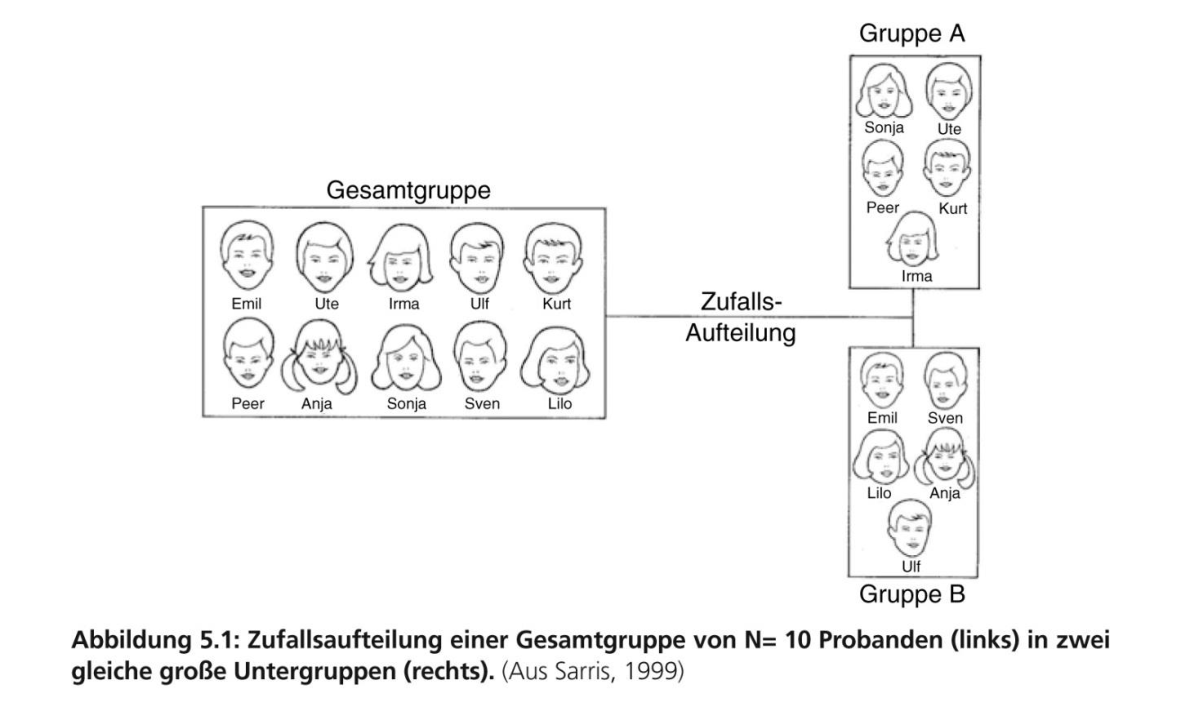
\includegraphics[width=0.85\linewidth]{8_Abbildungen/alm_8_randomisierung} \end{center}
\vfill
\end{frame}

\begin{frame}{Grundbegriffe}
\protect\hypertarget{grundbegriffe-8}{}
\setstretch{1.5}

\textcolor{darkblue}{Designschemata}

\begin{itemize}
\tightlist
\item
  R: Randomisierung
\item
  O: Observation (Test, Messung)
\item
  X: Exposition experimenteller Bedingung
\item
  Experimentelle Bedingungen von oben nach unten
\item
  Zeitliche Abfolge von links nach rechts
\end{itemize}

\vspace{1mm}

\textcolor{darkblue}{Beispiel}

\center
\begin{tabular}{|ccc|}
\hline
$\quad$R$\quad$  & $\quad$X$\quad$ & $\quad$O$\quad$
\\
$\quad$R$\quad$  & $\quad$ $\quad$ & $\quad$O$\quad$
\\\hline
\end{tabular}
\vspace{2mm}

\begin{itemize}
\tightlist
\item
  \small Bedingungszuweisung erfolgt durch Randomisierung
\item
  Nur eine Gruppe erhält das Treatment
\item
  Beide Gruppen absolvieren die Messung
\end{itemize}
\end{frame}

\begin{frame}[plain]{}
\protect\hypertarget{section-4}{}
\vfill
\large
\setstretch{2.5}

Grundbegriffe

\textbf{Randomisierte einfaktorielle Studiendesigns}

Randomisierte mehrfaktorielle Studiendesigns

Anwendungskontext

Anwendungsbeispiel

Selbstkontrollfragen \vfill
\end{frame}

\begin{frame}{Randomisierte einfaktorielle Studiendesigns}
\protect\hypertarget{randomisierte-einfaktorielle-studiendesigns}{}
\setstretch{1.8}

\textcolor{darkblue}{Randomisierte einfaktorielle Studiendesigns}

\begin{itemize}
\tightlist
\item
  Gesamtgruppe wird zufällig auf experimentelle Bedingungen aufgeteilt
\item
  Eine unabhängige Variable mit zwei oder mehr Leveln
\item
  Populäres Designs in der klinischen Forschung
\item
  Varianten

  \begin{itemize}
  \item[o] Treatment- und Kontrollgruppe
  \item[o] Treatment- und Placebogruppe
  \item[o] Zwei Treatmentgruppen (und Kontrollgruppe)
  \item[o] Pretest-Posttest Designs
  \end{itemize}
\end{itemize}
\end{frame}

\begin{frame}{Randomisierte einfaktorielle Studiendesigns}
\protect\hypertarget{randomisierte-einfaktorielle-studiendesigns-1}{}
\setstretch{2}
\large

\textcolor{darkblue}{No-Treatment Kontrollgruppe} \vspace{4mm}

\center
\begin{tabular}{|ccc|}
\hline
$\quad$R$\quad$  & $\quad$X$\quad$ & $\quad$O$\quad$
\\
$\quad$R$\quad$  & $\quad$ $\quad$ & $\quad$O$\quad$
\\\hline
\end{tabular}
\vspace{2mm}

\normalsize

\begin{itemize}
\tightlist
\item
  Vergleich eines Treatments zu keinem Treatment
\end{itemize}
\end{frame}

\begin{frame}{Randomisierte einfaktorielle Studiendesigns}
\protect\hypertarget{randomisierte-einfaktorielle-studiendesigns-2}{}
\setstretch{2}
\large

\textcolor{darkblue}{Placebo Kontrollgruppe} \vspace{6mm}

\large
\center
\begin{tabular}{|clc|}
\hline
$\quad$R$\quad$  & $\quad$X     $\quad$ & $\quad$O$\quad$
\\
$\quad$R$\quad$  & $\quad$X$_P$ $\quad$ & $\quad$O$\quad$
\\\hline
\end{tabular}
\vspace{6mm}

\normalsize

\begin{itemize}
\tightlist
\item
  Placebo = Scheintreatment
\item
  Vergleich eines Treatments zu keinem Treatment
\item
  Kontrolle studieninduzierter Effekte (Placeboeffekte)
\end{itemize}
\end{frame}

\begin{frame}{Randomisierte einfaktorielle Studiendesigns}
\protect\hypertarget{randomisierte-einfaktorielle-studiendesigns-3}{}
\setstretch{2}
\large

\textcolor{darkblue}{Vergleich zweier Treatments} \vspace{6mm}

\large
\center
\begin{tabular}{|clc|}
\hline
$\quad$R$\quad$  & $\quad$X$_A$ $\quad$ & $\quad$O$\quad$
\\
$\quad$R$\quad$  & $\quad$X$_B$ $\quad$ & $\quad$O$\quad$
\\\hline
\end{tabular}
\vspace{6mm}

\normalsize

\begin{itemize}
\tightlist
\item
  Vergleich Standardtreatment A und neues Treatment B
\item
  Keine Aussage über Effektivität des Standardtreatments
\end{itemize}
\end{frame}

\begin{frame}{Randomisierte einfaktorielle Studiendesigns}
\protect\hypertarget{randomisierte-einfaktorielle-studiendesigns-4}{}
\large

\textcolor{darkblue}{Zwei-Treatment Vergleich mit Placebo-Kontrollgruppe}
\vspace{4mm}

\center
\begin{tabular}{|clc|}
\hline
$\quad$R$\quad$  & $\quad$X$_A$ $\quad$ & $\quad$O$\quad$
\\
$\quad$R$\quad$  & $\quad$X$_B$ $\quad$ & $\quad$O$\quad$
\\
$\quad$R$\quad$  & $\quad$X$_P$ $\quad$ & $\quad$O$\quad$
\\\hline
\end{tabular}
\vspace{2mm}

\normalsize

\begin{itemize}
\tightlist
\item
  Vergleich Standardtreatment A und neues Treatment B
\item
  Aussage über Effektivität des Standardtreatments möglich
\item
  Placebotreatment kann ethisch nicht vertretbar sein
\end{itemize}

\small
\flushleft

Beispiel: Einfluss von Psychotherapie auf Depressionssymptomatik

\begin{itemize}
\tightlist
\item
  Klassische Psychotherapie (A)
\item
  Online Psychotherapie (B)
\item
  Seelsorge (P)
\end{itemize}

\normalsize

\textcolor{darkblue}{$\quad\quad\rightarrow$ Keine Aussagen über Pre-Treatment Gruppenunterschiede möglich}

\textcolor{darkblue}{$\quad\quad\rightarrow$ Keine Aussage über Dropout Charakteristika möglich}
\end{frame}

\begin{frame}{Randomisierte einfaktorielle Studiendesigns}
\protect\hypertarget{randomisierte-einfaktorielle-studiendesigns-5}{}
\large
\setstretch{2}

\textcolor{darkblue}{Pre-Posttest Designs} \vspace{4mm}

\center
\begin{tabular}{|cclc|}
\hline
$\quad$R$\quad$ & $\quad$O$\quad$ & $\quad$X$_A$ $\quad$ & $\quad$O$\quad$
\\
$\quad$R$\quad$ & $\quad$O$\quad$ & $\quad$X$_B$ $\quad$ & $\quad$O$\quad$
\\
$\quad$R$\quad$ & $\quad$O$\quad$ & $\quad$      $\quad$ & $\quad$O$\quad$
\\\hline
\end{tabular}
\vspace{6mm}

\normalsize

\begin{itemize}
\tightlist
\item
  Fokus auf Treatment-induzierte Verbesserungen/Verschlechterungen
\item
  Subtraktion von Pre-Test-Gruppenunterschieden möglich
\item
  Untersuchung von Dropout Charakteristika möglich
\item
  Mögliches Auftreten von Testeffekten (Lernen, Gewöhnung, Ermüdung)
\item
  Höherer Zeit- und Kostenaufwand
\end{itemize}
\end{frame}

\begin{frame}{Randomisierte einfaktorielle Studiendesigns}
\protect\hypertarget{randomisierte-einfaktorielle-studiendesigns-6}{}
\textcolor{darkblue}{Beispiel: Evaluation von Psychotherapieformen bei Depression}
\vspace{2mm}

\begin{center}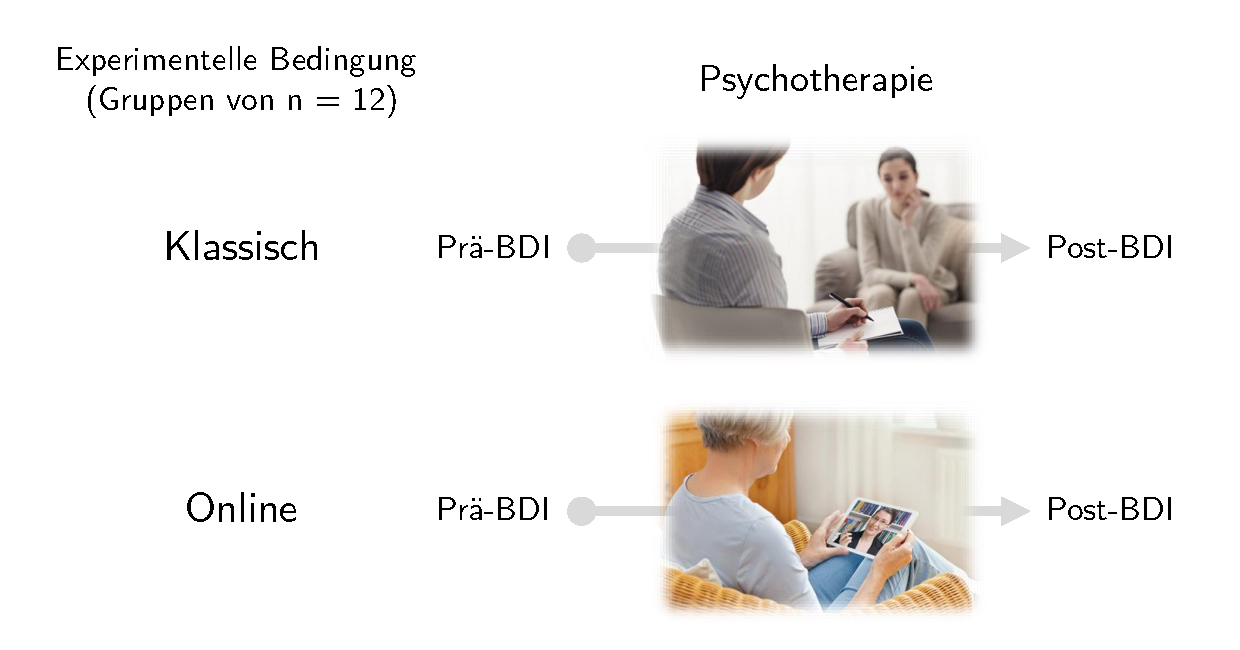
\includegraphics[width=0.9\linewidth]{8_Abbildungen/alm_8_messplan} \end{center}

\large
\center

\(\Rightarrow\) Randomisiertes einfaktorielles Preposttest Design ohne
Kontrollgruppe
\end{frame}

\begin{frame}[plain]{}
\protect\hypertarget{section-5}{}
\vfill
\large
\setstretch{2.5}

Grundbegriffe

Randomisierte einfaktorielle Studiendesigns

\textbf{Randomisierte mehrfaktorielle Studiendesigns}

Anwendungskontext

Anwendungsbeispiel

Selbstkontrollfragen \vfill
\end{frame}

\begin{frame}{Randomisierte mehrfaktorielle Studiendesigns}
\protect\hypertarget{randomisierte-mehrfaktorielle-studiendesigns}{}
\setstretch{2}

\textcolor{darkblue}{Mehrfaktorielle Studiendesigns}

\begin{itemize}
\tightlist
\item
  Kombination mehrerer experimenteller Faktoren in einem Versuchsplan
\end{itemize}

\textcolor{darkblue}{Crossed Design}

\begin{itemize}
\tightlist
\item
  Jedes Level jedes Faktors wird mit allen Leveln aller Faktoren
  kombiniert.
\end{itemize}

\textcolor{darkblue}{Nested Design}

\begin{itemize}
\tightlist
\item
  Einige Level eines Faktors werden nicht mit allen anderen Faktorleveln
  kombiniert.
\end{itemize}

\center

\textcolor{darkblue}{$\Rightarrow$ Prototypisch sind zweifaktorielle Studiendesigns mit crossed design}
\end{frame}

\begin{frame}{Randomisierte mehrfaktorielle Studiendesigns}
\protect\hypertarget{randomisierte-mehrfaktorielle-studiendesigns-1}{}
\setstretch{1.4}

\textcolor{darkblue}{Randomisiertes zweifaktorieller Studiendesigns mit crossed design}

\small

\begin{itemize}
\tightlist
\item
  Eine univariate abhängige Variable bestimmt an individuellen
  experimentellen Einheiten.
\item
  Zwei diskrete unabhängige Variablen, die mindestens zweistufig sind.
\item
  Die unabhängigen Variablen werden \textit{Faktoren} genannt.
\item
  Die Stufen der Faktoren werden \textit{Level} genannt.
\item
  Jedes Level eines Faktors wird mit allen Level des anderen Faktors
  kombiniert
\end{itemize}

\normalsize

\textcolor{darkblue}{Zweifaktorielle Studiendesigns werden üblicherweise anhand ihrer Faktorlevel bezeichnet}

\small
\begin{center}
\begin{tabular}{lll}
2 x 2 Design: Faktor A mit Level 1,2     & Faktor B mit Level 1,2       \\
2 x 3 Design: Faktor A mit Level 1,2     & Faktor B mit Level 1,2,3     \\
4 x 2 Design: Faktor A mit Level 1,2,3,4 & Faktor B mit Level 1,2       \\
3 x 1 Design: Faktor A mit Level 1,2,3   & Faktor B mit Level 1
\end{tabular}
\end{center}

\begin{itemize}
\tightlist
\item
  2 x 2 Studiendesigns sind sehr populär, wir fokussieren auf diesen
  Fall.
\end{itemize}

\normalsize

\(\Rightarrow\) Das entsprechende datenanalytische Verfahren ist die
Varianzanalyse (ANOVA)
\end{frame}

\begin{frame}{Randomisierte mehrfaktorielle Studiendesigns}
\protect\hypertarget{randomisierte-mehrfaktorielle-studiendesigns-2}{}
\textcolor{darkblue}{Konzeptuelles Design eines 2 x 2 Versuchsplans}

\begin{center}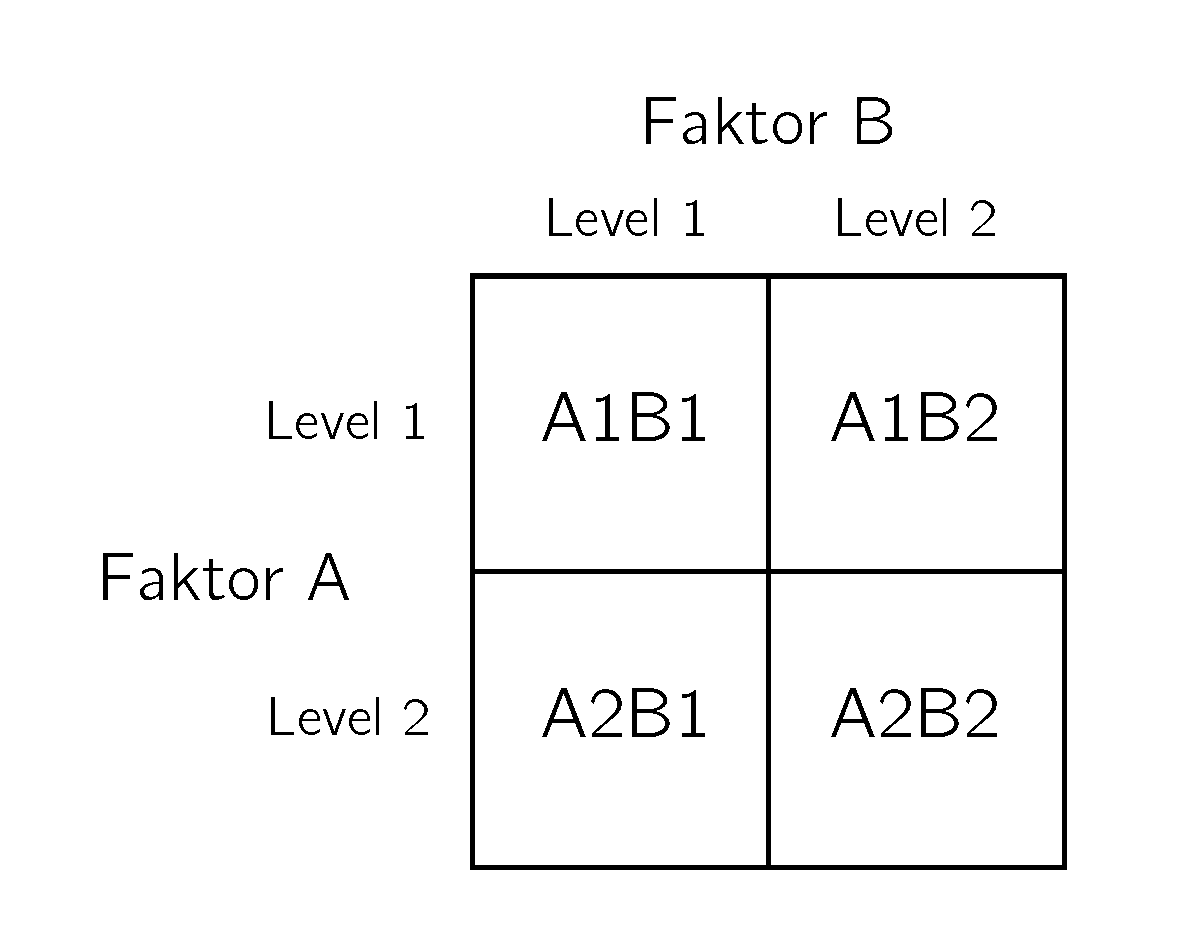
\includegraphics[width=0.65\linewidth]{8_Abbildungen/alm_8_zweifaktorielle_va_nomenklatur} \end{center}
\end{frame}

\begin{frame}{Randomisierte mehrfaktorielle Studiendesigns}
\protect\hypertarget{randomisierte-mehrfaktorielle-studiendesigns-3}{}
\textcolor{darkblue}{Anwendungsbeispiel eines randomisierten 2 x 2 Versuchsplans}
\small \setstretch{1.6}

\begin{itemize}
\tightlist
\item
  Ist Psychotherapie bei Depression im klassischen oder im online
  Setting wirksamer?
\item
  Ist Psychotherapie bei bei Depression bei jüngeren oder älterne
  Patient:innen wirksamer?
\end{itemize}

\begin{center}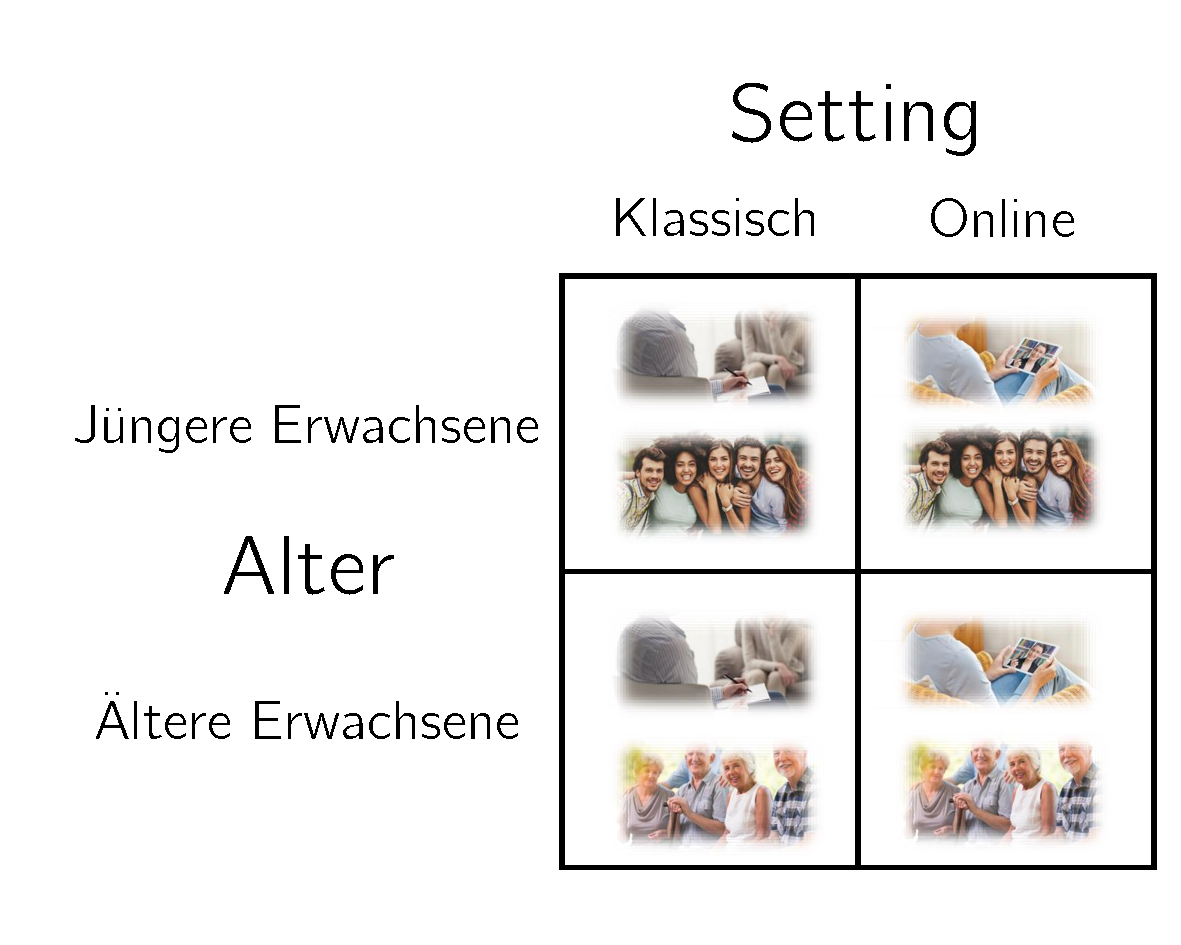
\includegraphics[width=0.5\linewidth]{8_Abbildungen/alm_8_zweifaktorielle_va_beispiel} \end{center}

\begin{itemize}
\tightlist
\item
  Ist die Wirksamkeit der Psychotherapie vom Setting abhängig?
\item
  Ist die Wirksamkeit der Psychotherapie vom Alter der Patient:innen
  abhängig?
\end{itemize}
\end{frame}

\begin{frame}{Randomisierte mehrfaktorielle Studiendesigns}
\protect\hypertarget{randomisierte-mehrfaktorielle-studiendesigns-4}{}
\textcolor{darkblue}{Verlaufsschema eines randomisierten 2 x 2 Versuchsplans}
\vspace{1cm}

\center
\large
\begin{tabular}{|clc|}
\hline
$\quad$R$\quad$  & $\quad$X$_{A1B1}$ $\quad$ & $\quad$O$\quad$
\\
$\quad$R$\quad$  & $\quad$X$_{A1B2}$ $\quad$ & $\quad$O$\quad$
\\
$\quad$R$\quad$  & $\quad$X$_{A2B1}$ $\quad$ & $\quad$O$\quad$
\\
$\quad$R$\quad$  & $\quad$X$_{A2B2}$ $\quad$ & $\quad$O$\quad$
\\\hline
\end{tabular}
\vspace{1cm}

\normalsize
\setstretch{2}

\begin{itemize}
\tightlist
\item
  Pre-Posttest Designs möglich
\item
  Placebo Kontrollgruppen möglich
\end{itemize}
\end{frame}

\begin{frame}{Randomisierte mehrfaktorielle Studiendesigns}
\protect\hypertarget{randomisierte-mehrfaktorielle-studiendesigns-5}{}
\textcolor{darkblue}{Daten bei 2 x 2 Studiendesignsn}

\begin{center}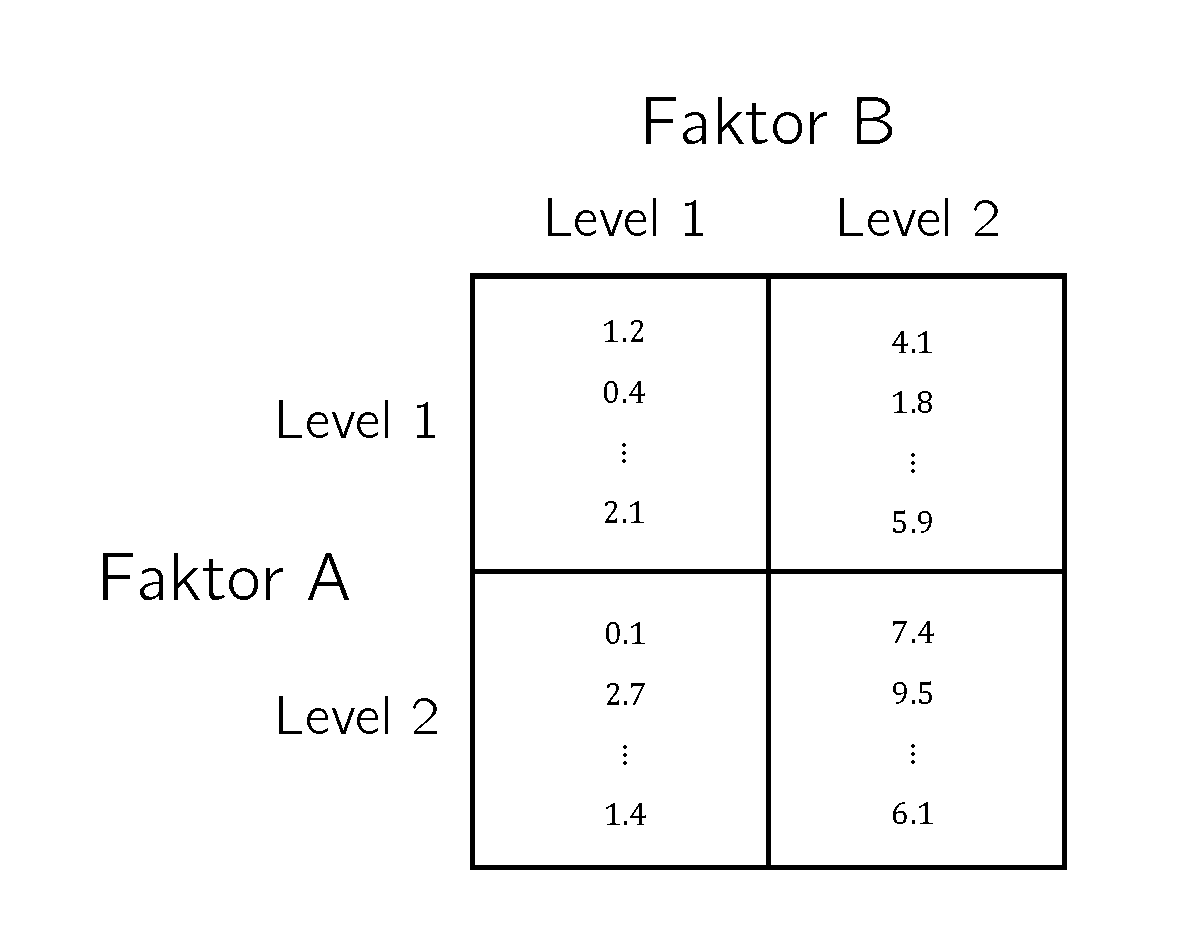
\includegraphics[width=0.7\linewidth]{8_Abbildungen/alm_8_zweifaktorielle_va_konzept} \end{center}
\end{frame}

\begin{frame}{Randomisierte mehrfaktorielle Studiendesigns}
\protect\hypertarget{randomisierte-mehrfaktorielle-studiendesigns-6}{}
\textcolor{darkblue}{Haupteffekte und Interaktionen}

\footnotesize
\justifying

Hinsichtlich der Gruppenmittelwerte bei 2 x 2 Studiendesignsn
unterscheidet man \textbf{Haupteffekte} und \textbf{Interaktionen}

\begin{itemize}
\item
  Intuitiv spricht man vom Vorliegen eines
  \textit{Haupteffekts von Faktor A}, wenn sich die Gruppenmittelwerte
  zwischen Level 1 und Level 2 von Faktor A, jeweils gemittelt über die
  zwei Level von Faktor B, unterscheiden.
\item
  Intuitiv spricht man vom Vorliegen eines
  \textit{Haupteffekts von Faktor B}, wenn sich die Gruppenmittelwerte
  zwischen Level 1 und Level 2 von Faktor B, jeweils gemittelt über die
  zwei Level von Faktor A, unterscheiden.
\item
  Intuitiv spricht man vom Vorliegen einer
  \textit{Interaktion der Faktoren A
  und B}, wenn der Unterschied der Gruppenmittelwerte von Faktor A
  zwischen Level 1 und 2 unterschiedlich für Level 1 und Level 2 von
  Faktor B ausgeprägt ist bzw. wenn der Unterschied der
  Gruppenmittelwerte von Faktor B zwischen Level 1 und 2 unterschiedlich
  für Level 1 und Level 2 von Faktor A ausgeprägt ist.
\end{itemize}

Intuitiv beziehen sich Haupteffekte also auf (marginale) Unterschiede
(Differenzen), während sich Interaktionen auf Unterschiede von
Unterschieden (Differenzen von Differenzen) beziehen.

Das Vorhandensein einer Interaktion besagt lediglich, dass sich die
Unterschiede der Gruppenmittelwerte zwischen den Leveln eines
experimentellen Faktors in Abhängigkeit von den Leveln des anderen
experimentellen Faktors ändern, es macht aber keine Aussage darüber,
warum dies so ist. Haupteffekte und Interaktionen sind lediglich
Datenmuster, keine mechanistischen wissenschaftlichen Theorien.
\end{frame}

\begin{frame}[plain]{}
\protect\hypertarget{section-6}{}
\vfill
\large
\setstretch{2.5}

Grundbegriffe

Randomisierte einfaktorielle Studiendesigns

Randomisierte mehrfaktorielle Studiendesigns

\textbf{Anwendungskontext}

Anwendungsbeispiel

Selbstkontrollfragen \vfill
\end{frame}

\begin{frame}{Anwendungskontext}
\protect\hypertarget{anwendungskontext}{}
\textcolor{darkblue}{Evidenzbasierte Evaluation von Psychotherapieformen bei Depression}

\normalsize

Welche Therapieform ist bei Depression wirksamer?

\begin{center}
\includegraphics[width=1.1\linewidth]{8_Abbildungen/alm_8_klinische_forschung} \end{center}

\(\rightarrow\) Klinische Psychologie, Klinische Diagnostik, MSc
Psychotherapie

\footnotesize
\flushright

\emph{Wahrscheinlichkeitstheorie und Frequentistische Inferenz WiSe
21/22 (1) Einführung}
\end{frame}

\begin{frame}{Anwendungskontext}
\protect\hypertarget{anwendungskontext-1}{}
\textcolor{darkblue}{Evidenzbasierte Evaluation von Psychotherapieformen bei Depression}

\normalsize

Becks Depressions-Inventar (BDI) zur Depressionsdiagnostik

\begin{center}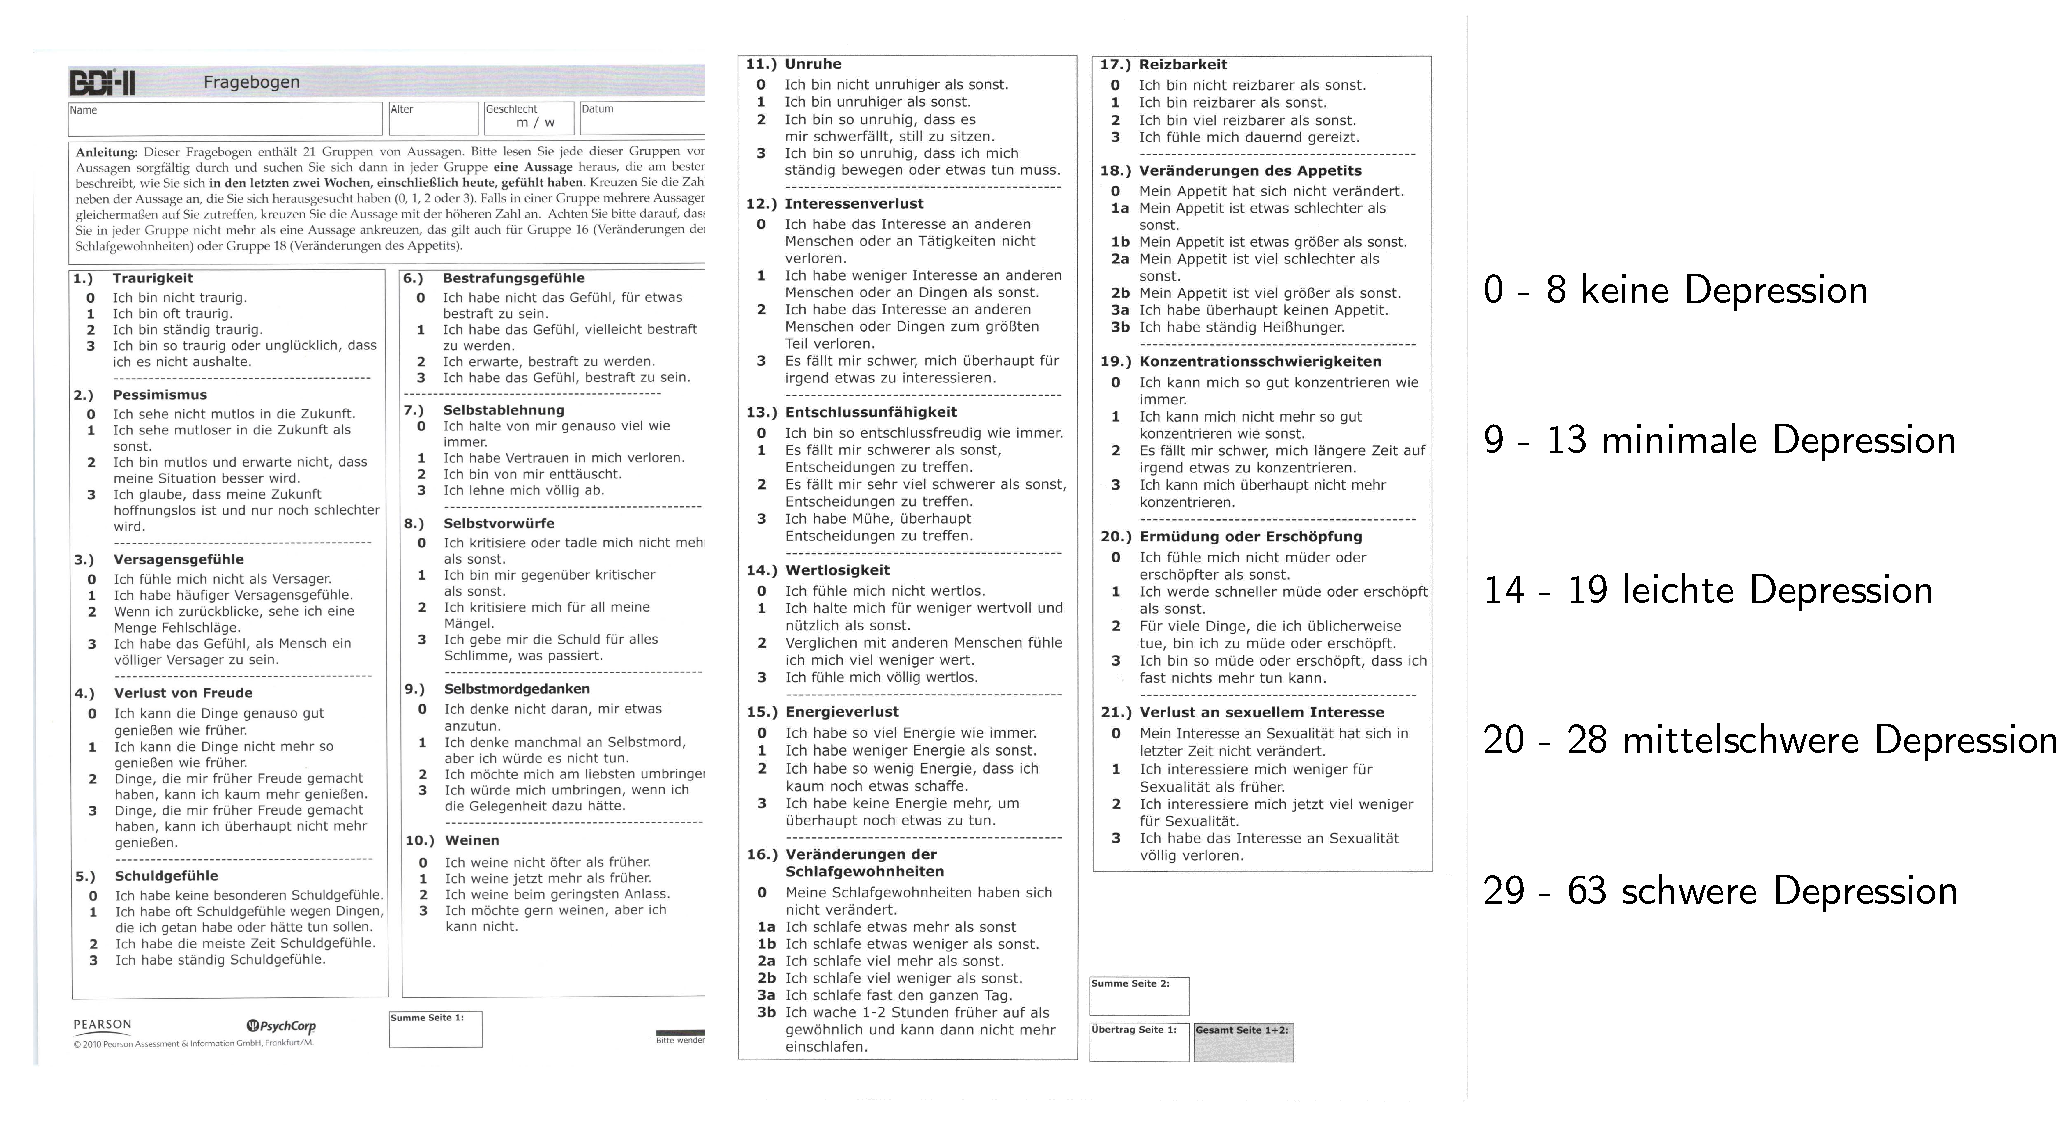
\includegraphics[width=0.95\linewidth]{8_Abbildungen/alm_8_bdi} \end{center}
\footnotesize
\flushright

\emph{Wahrscheinlichkeitstheorie und Frequentistische Inferenz WiSe
21/22 (1) Einführung}
\end{frame}

\begin{frame}{Anwendungskontext}
\protect\hypertarget{anwendungskontext-2}{}
\textcolor{darkblue}{Evidenzbasierte Evaluation von Psychotherapieformen bei Depression - Verhaltensdaten}

\footnotesize

\begin{longtable}[]{@{}cccc@{}}
\toprule
Patient ID & Bedingung & Prae-PT-BDI & Post-PT-BDI \\
\midrule
\endhead
1 & Online & 29 & 19 \\
2 & Online & 27 & 30 \\
3 & Klassisch & 16 & 11 \\
4 & Online & 19 & 26 \\
5 & Online & 35 & 29 \\
6 & Klassisch & 48 & 10 \\
7 & Online & 20 & 15 \\
8 & Online & 18 & 11 \\
9 & Online & 48 & 28 \\
10 & Klassisch & 49 & 23 \\
11 & Klassisch & 39 & 10 \\
12 & Online & 36 & 24 \\
13 & Online & 21 & 27 \\
14 & Online & 46 & 14 \\
15 & Online & 20 & 17 \\
16 & Klassisch & 23 & 10 \\
\bottomrule
\end{longtable}

\footnotesize
\flushright

\emph{Wahrscheinlichkeitstheorie und Frequentistische Inferenz WiSe
21/22 (1) Einführung}
\end{frame}

\begin{frame}[t]{Anwendungskontext}
\protect\hypertarget{anwendungskontext-3}{}
\begin{center}
\includegraphics[width=0.65\linewidth]{8_Abbildungen/alm_8_review_title} \end{center}
\center

\textcolor{darkblue}{Abstract}

\begin{center}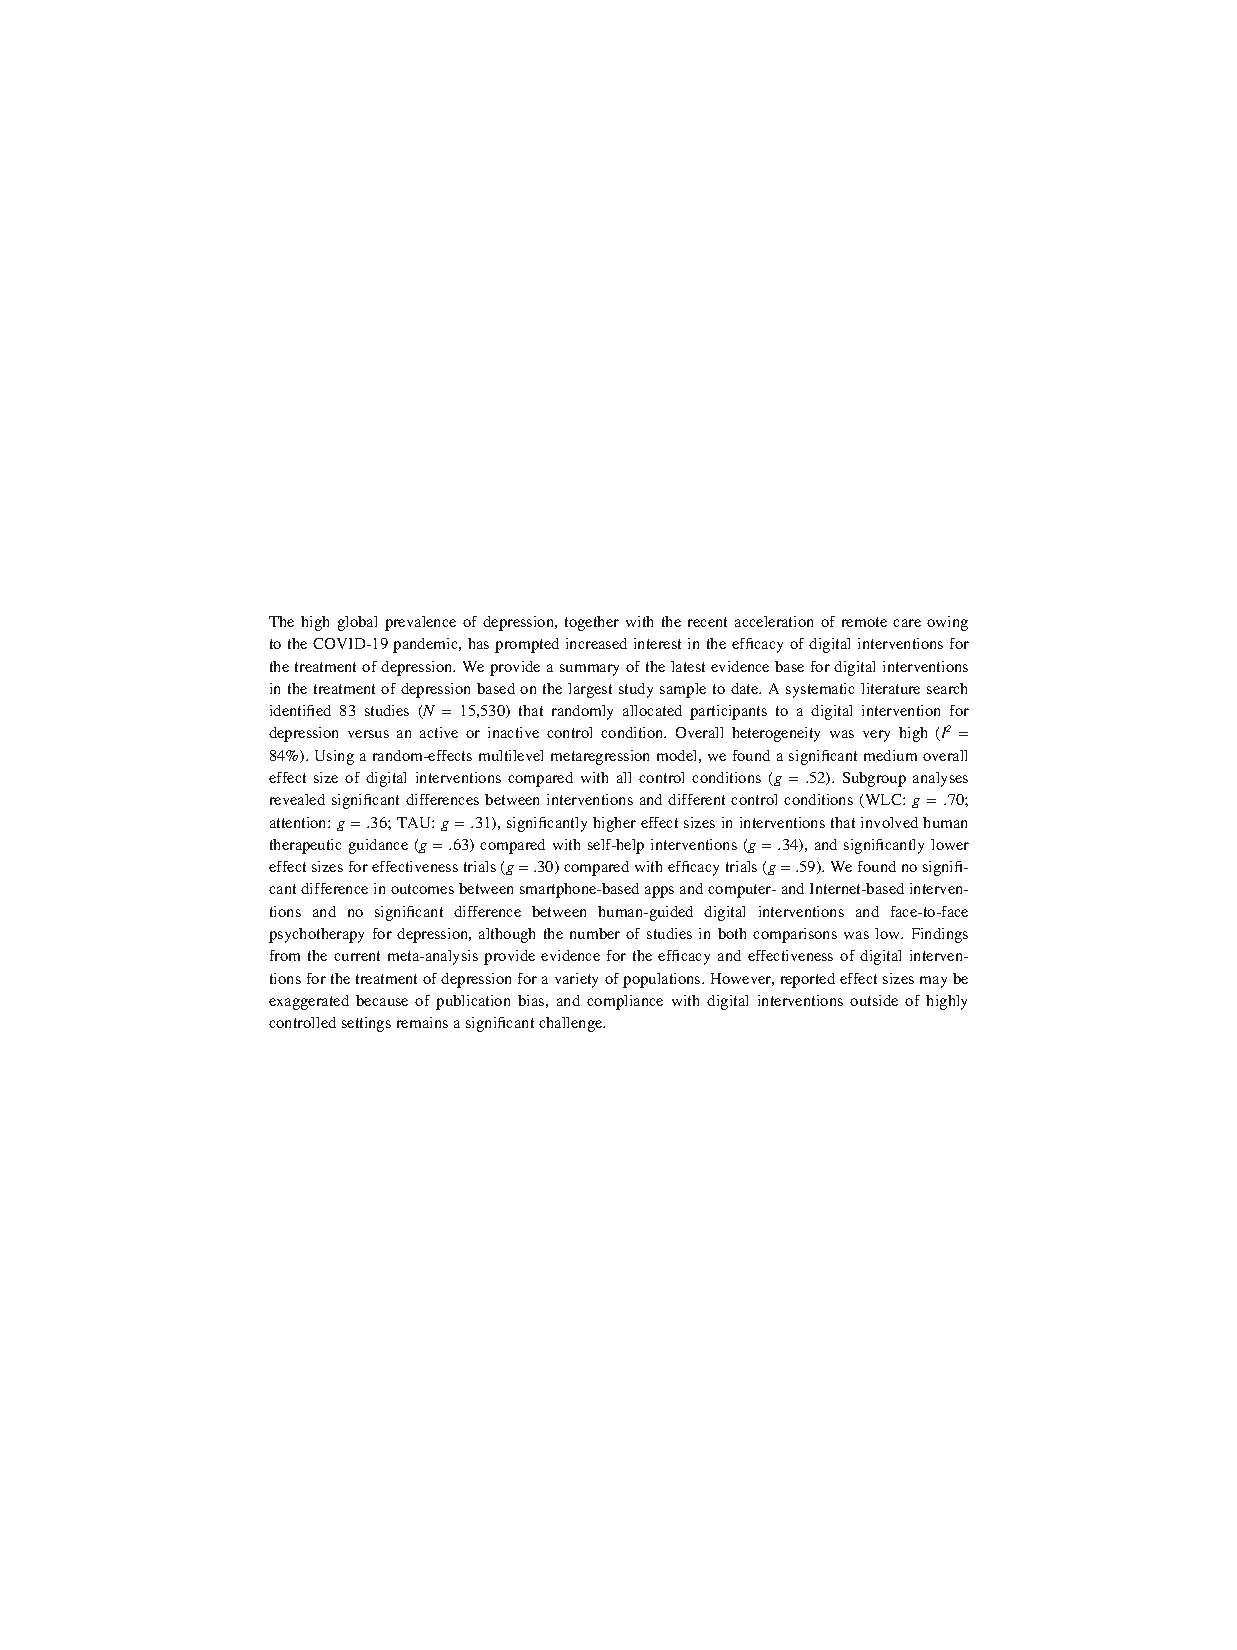
\includegraphics[width=0.65\linewidth]{8_Abbildungen/alm_8_review_abstract} \end{center}
\flushright
\footnotesize

\emph{Moshe et al. (2021)}
\end{frame}

\begin{frame}[t]{Anwendungskontext}
\protect\hypertarget{anwendungskontext-4}{}
\begin{center}
\includegraphics[width=0.7\linewidth]{8_Abbildungen/alm_8_review_title} \end{center}
\center

\textcolor{darkblue}{Results}

\begin{center}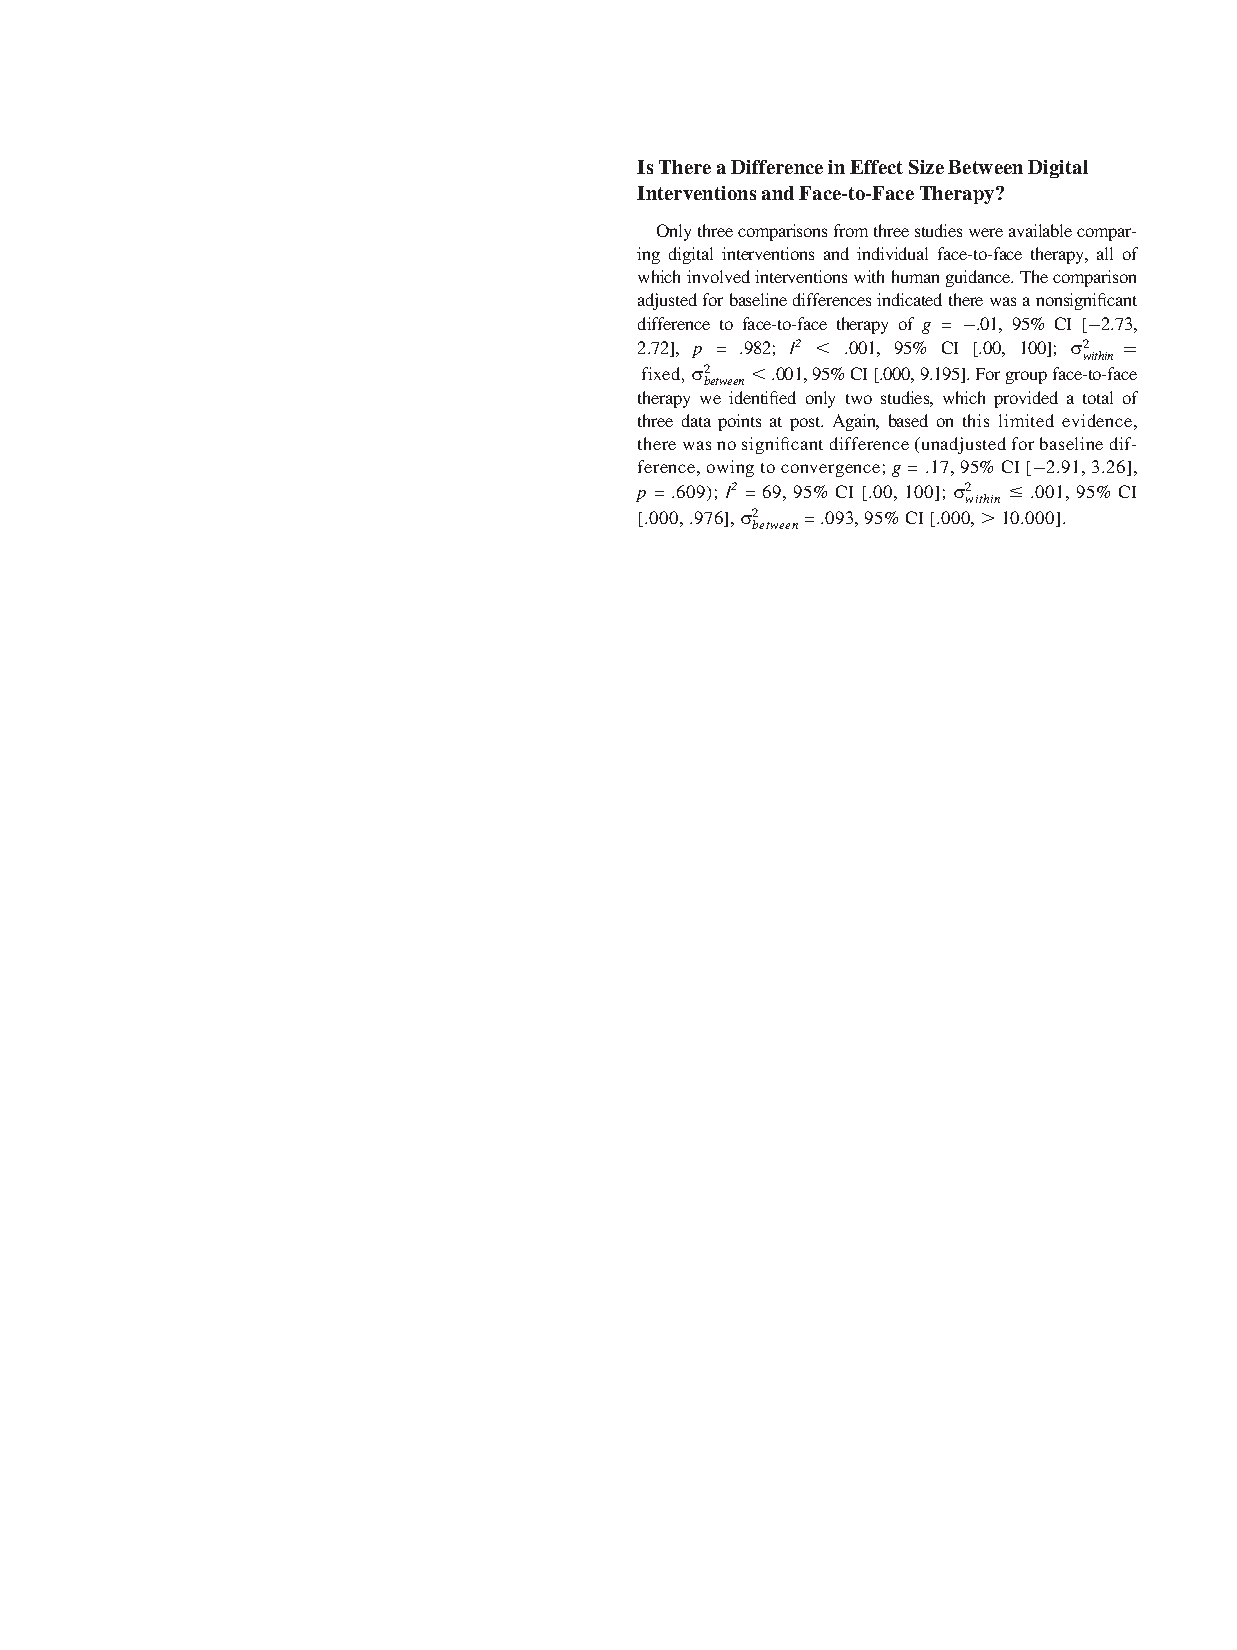
\includegraphics[width=0.5\linewidth]{8_Abbildungen/alm_8_review_results} \end{center}
\flushright
\footnotesize

\emph{Moshe et al. (2021)}
\end{frame}

\begin{frame}[t]{Anwendungskontext}
\protect\hypertarget{anwendungskontext-5}{}
\begin{center}
\includegraphics[width=0.7\linewidth]{8_Abbildungen/alm_8_review_title} \end{center}
\center

\textcolor{darkblue}{Discussion}

\begin{center}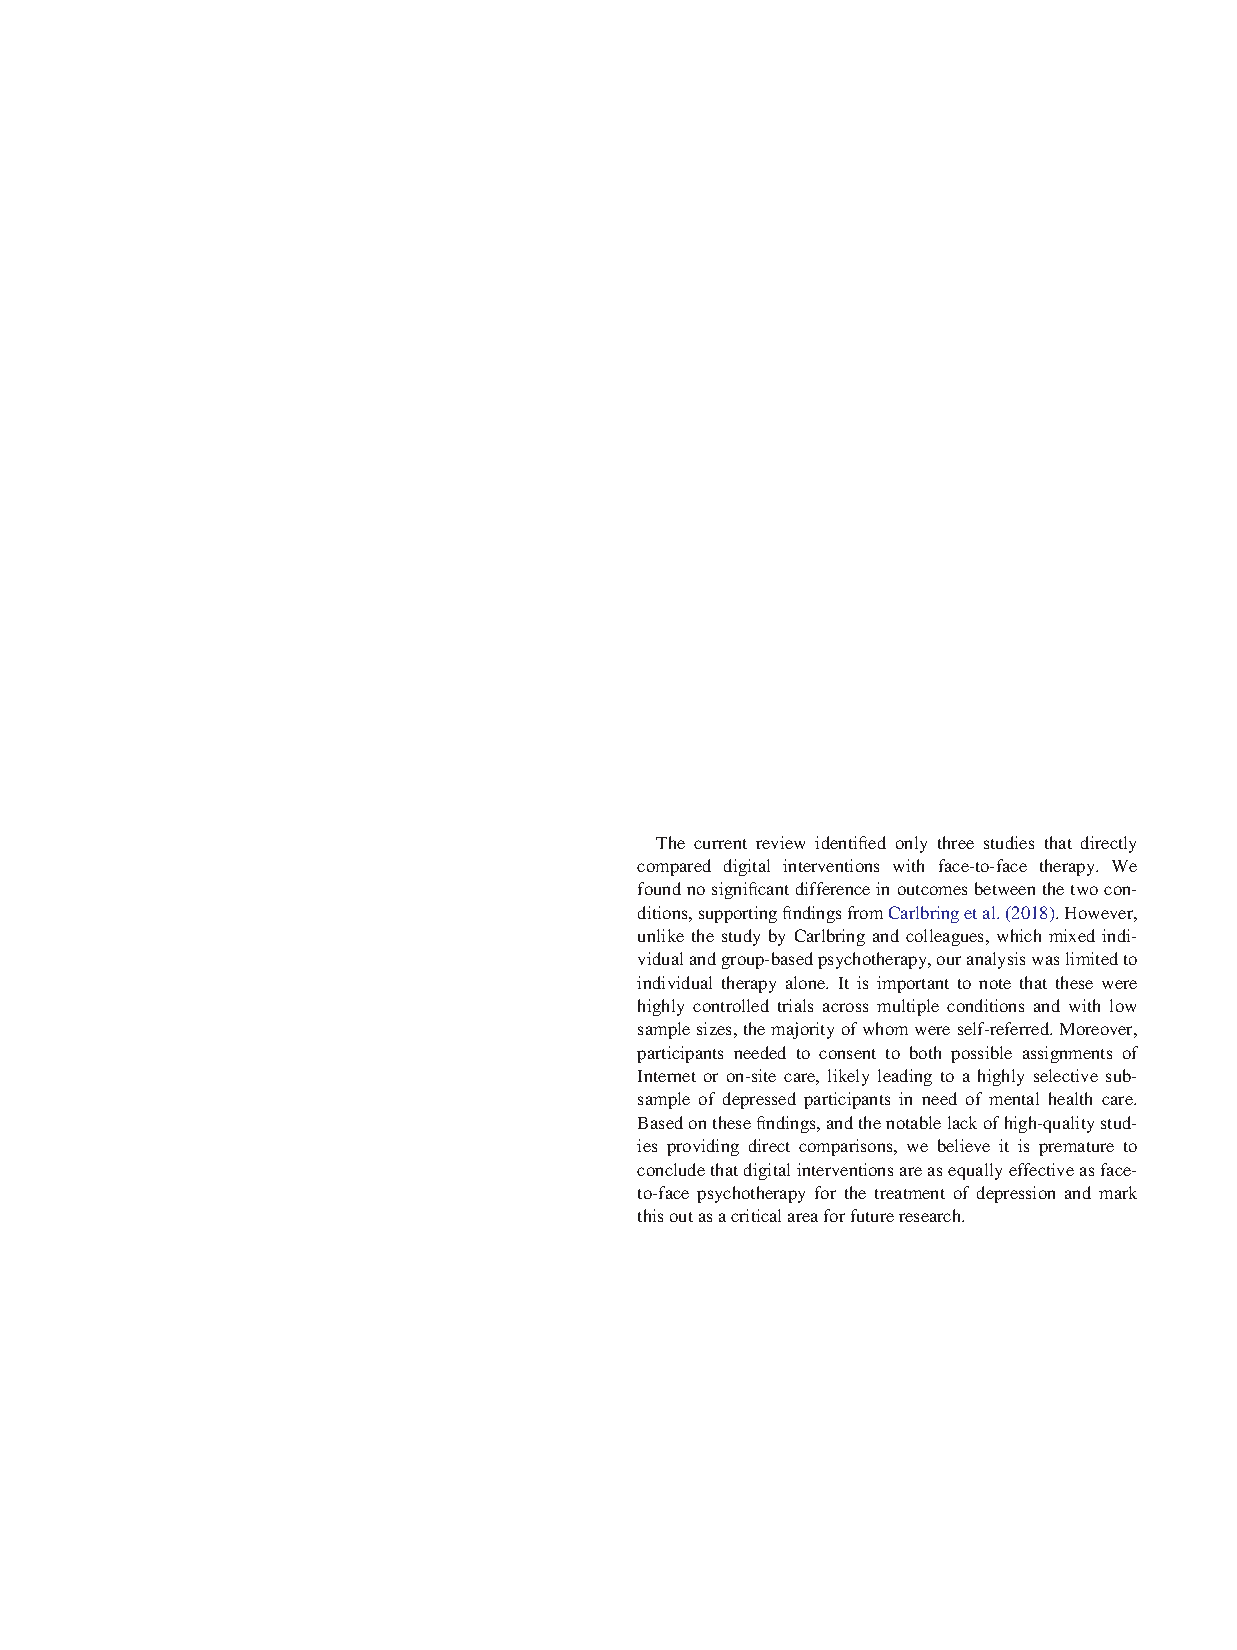
\includegraphics[width=0.5\linewidth]{8_Abbildungen/alm_8_review_discussion} \end{center}
\flushright
\footnotesize

\emph{Moshe et al. (2021)}
\end{frame}

\begin{frame}[t]{Anwendungskontext}
\protect\hypertarget{anwendungskontext-6}{}
\begin{center}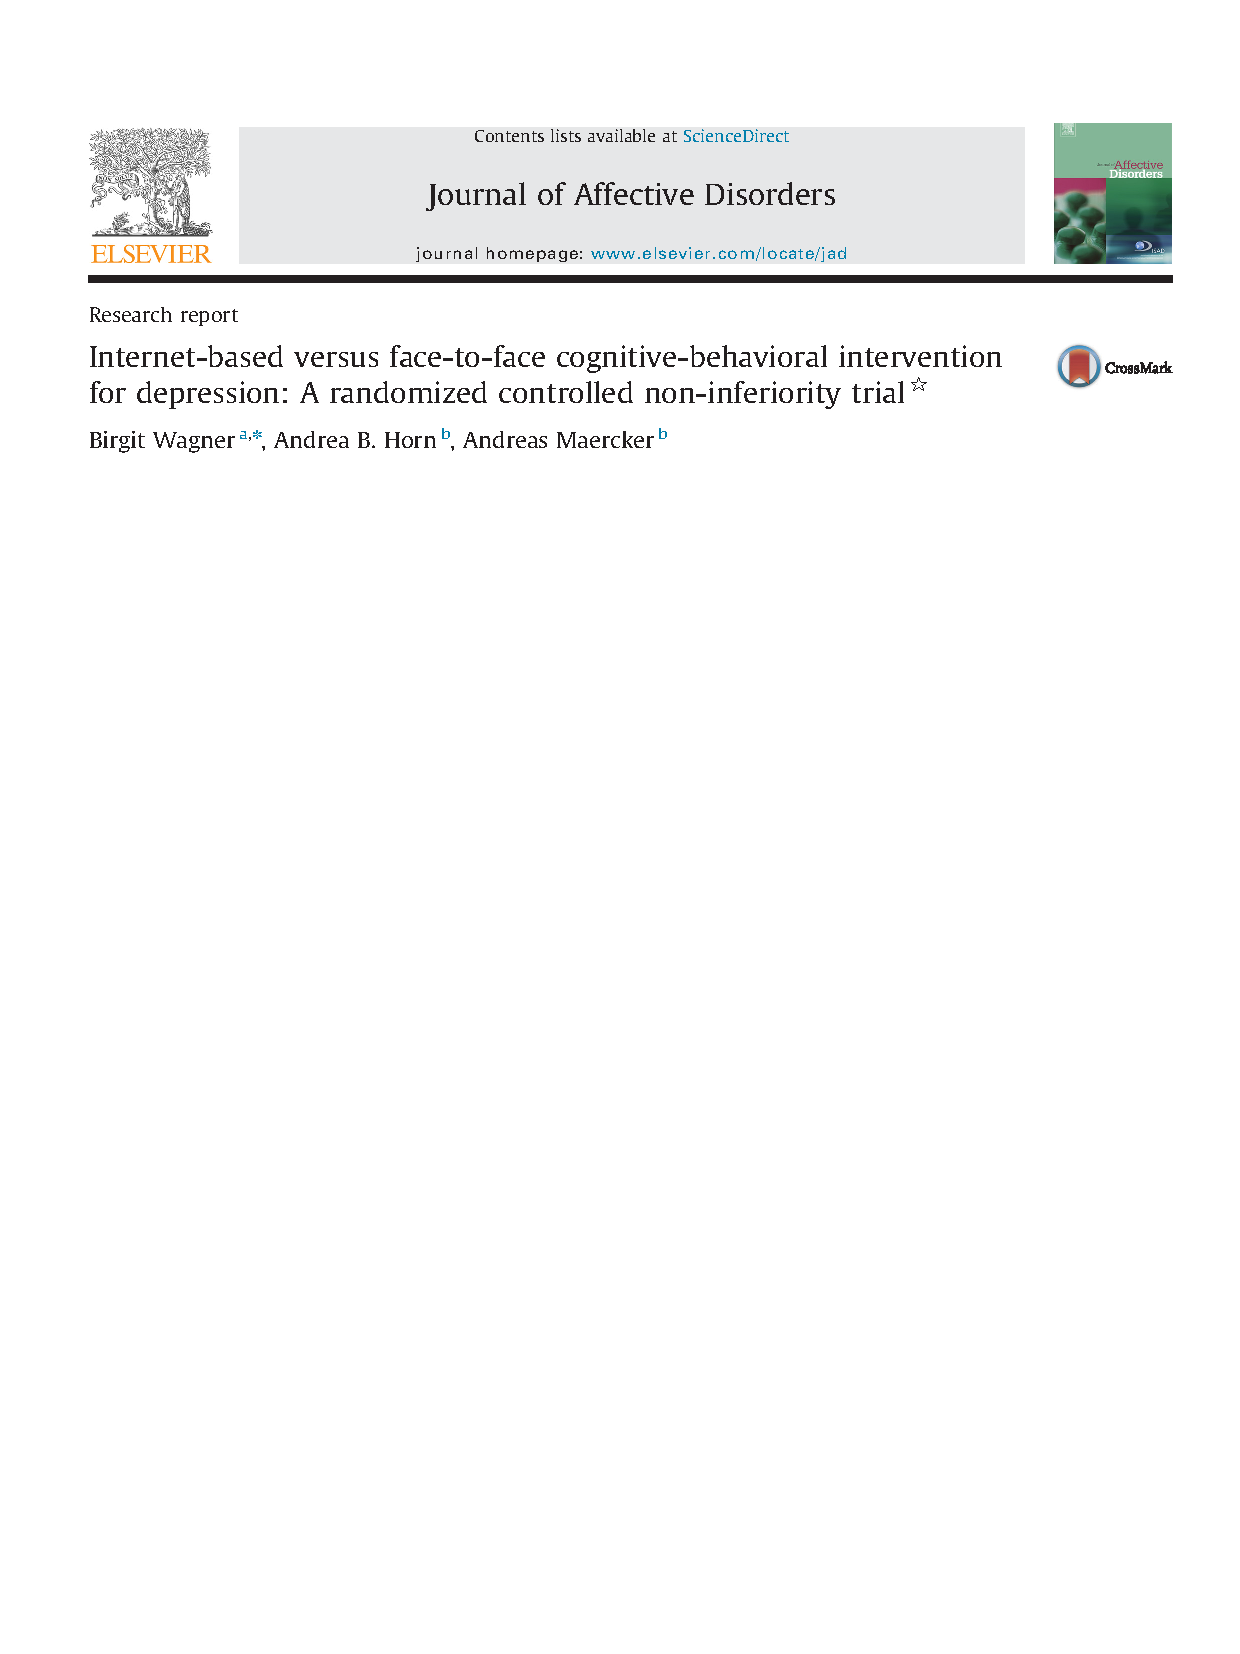
\includegraphics[width=0.5\linewidth]{8_Abbildungen/alm_8_article_title} \end{center}
\center

\textcolor{darkblue}{Abstract}

\begin{center}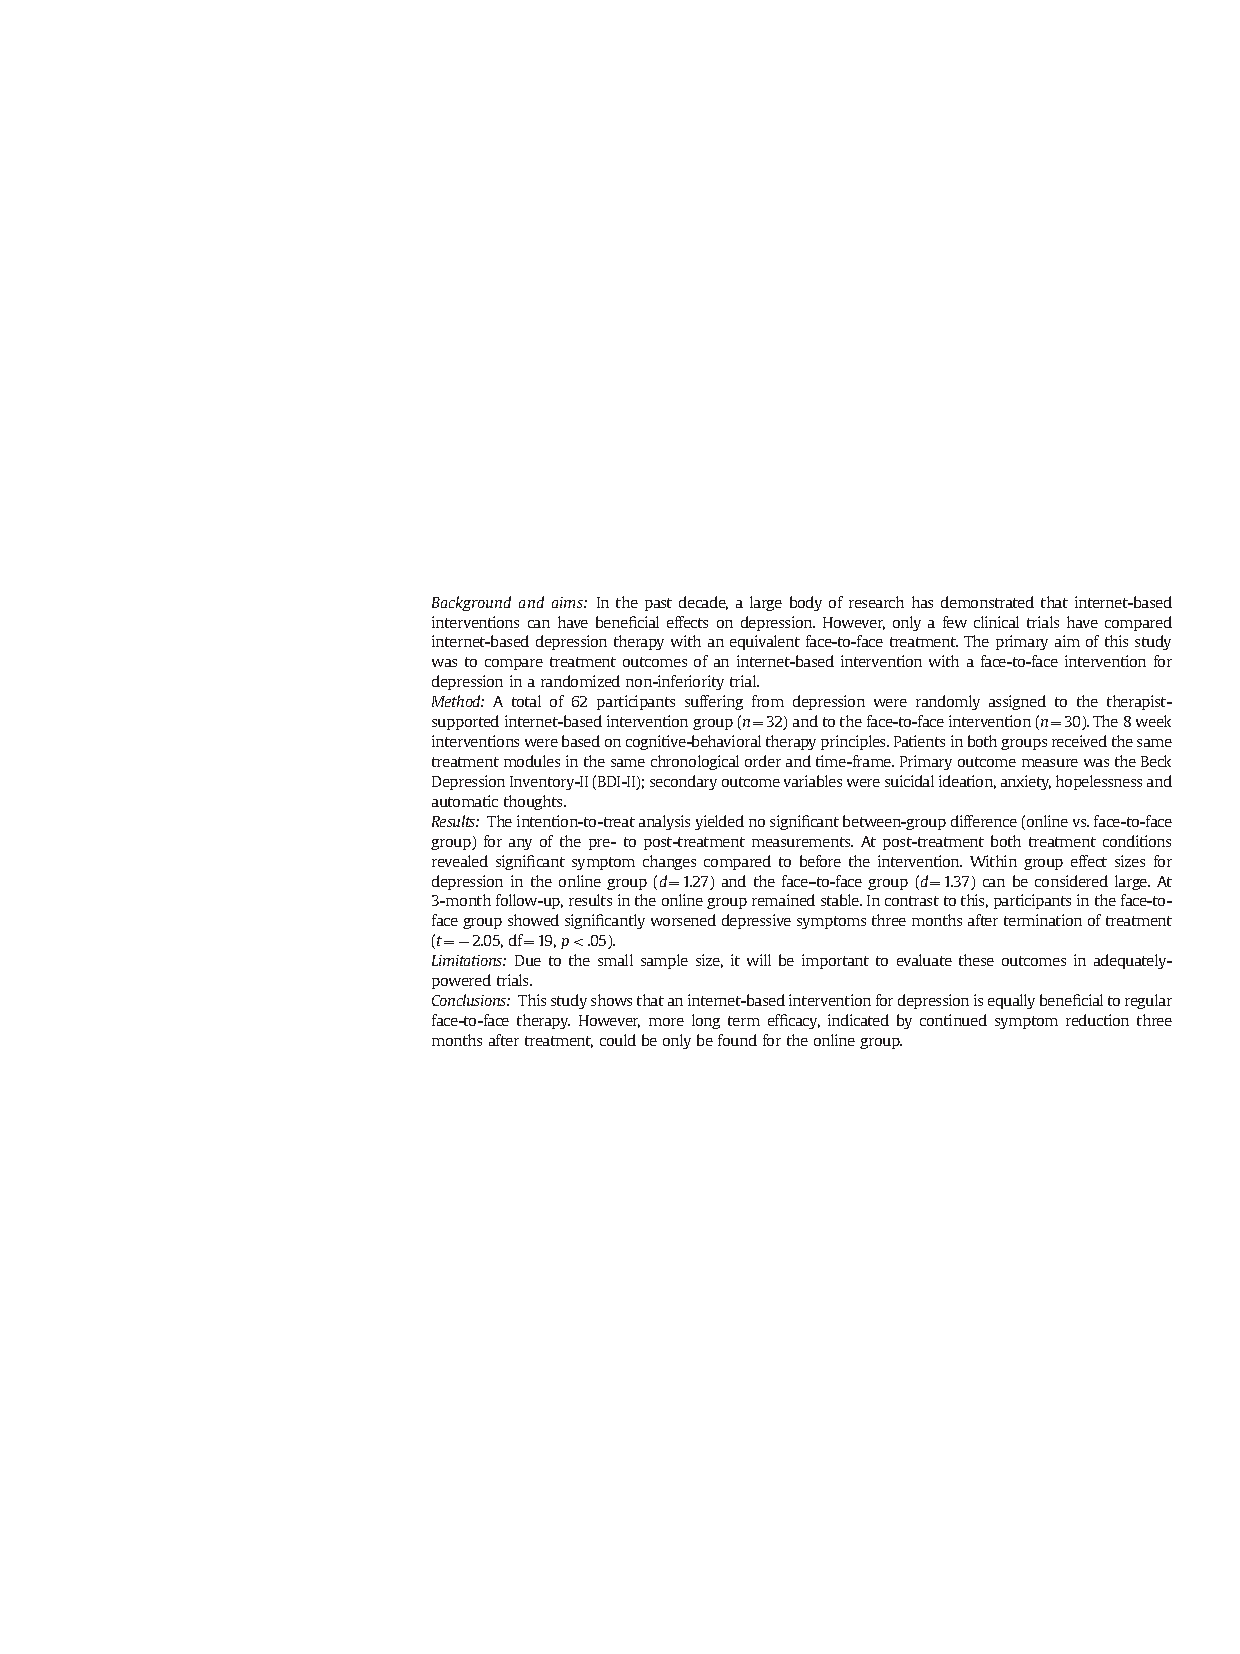
\includegraphics[width=0.7\linewidth]{8_Abbildungen/alm_8_article_abstract} \end{center}
\flushright
\footnotesize

\emph{Wagner, Horn, and Maercker (2014)}
\end{frame}

\begin{frame}[t]{Anwendungskontext}
\protect\hypertarget{anwendungskontext-7}{}
\begin{center}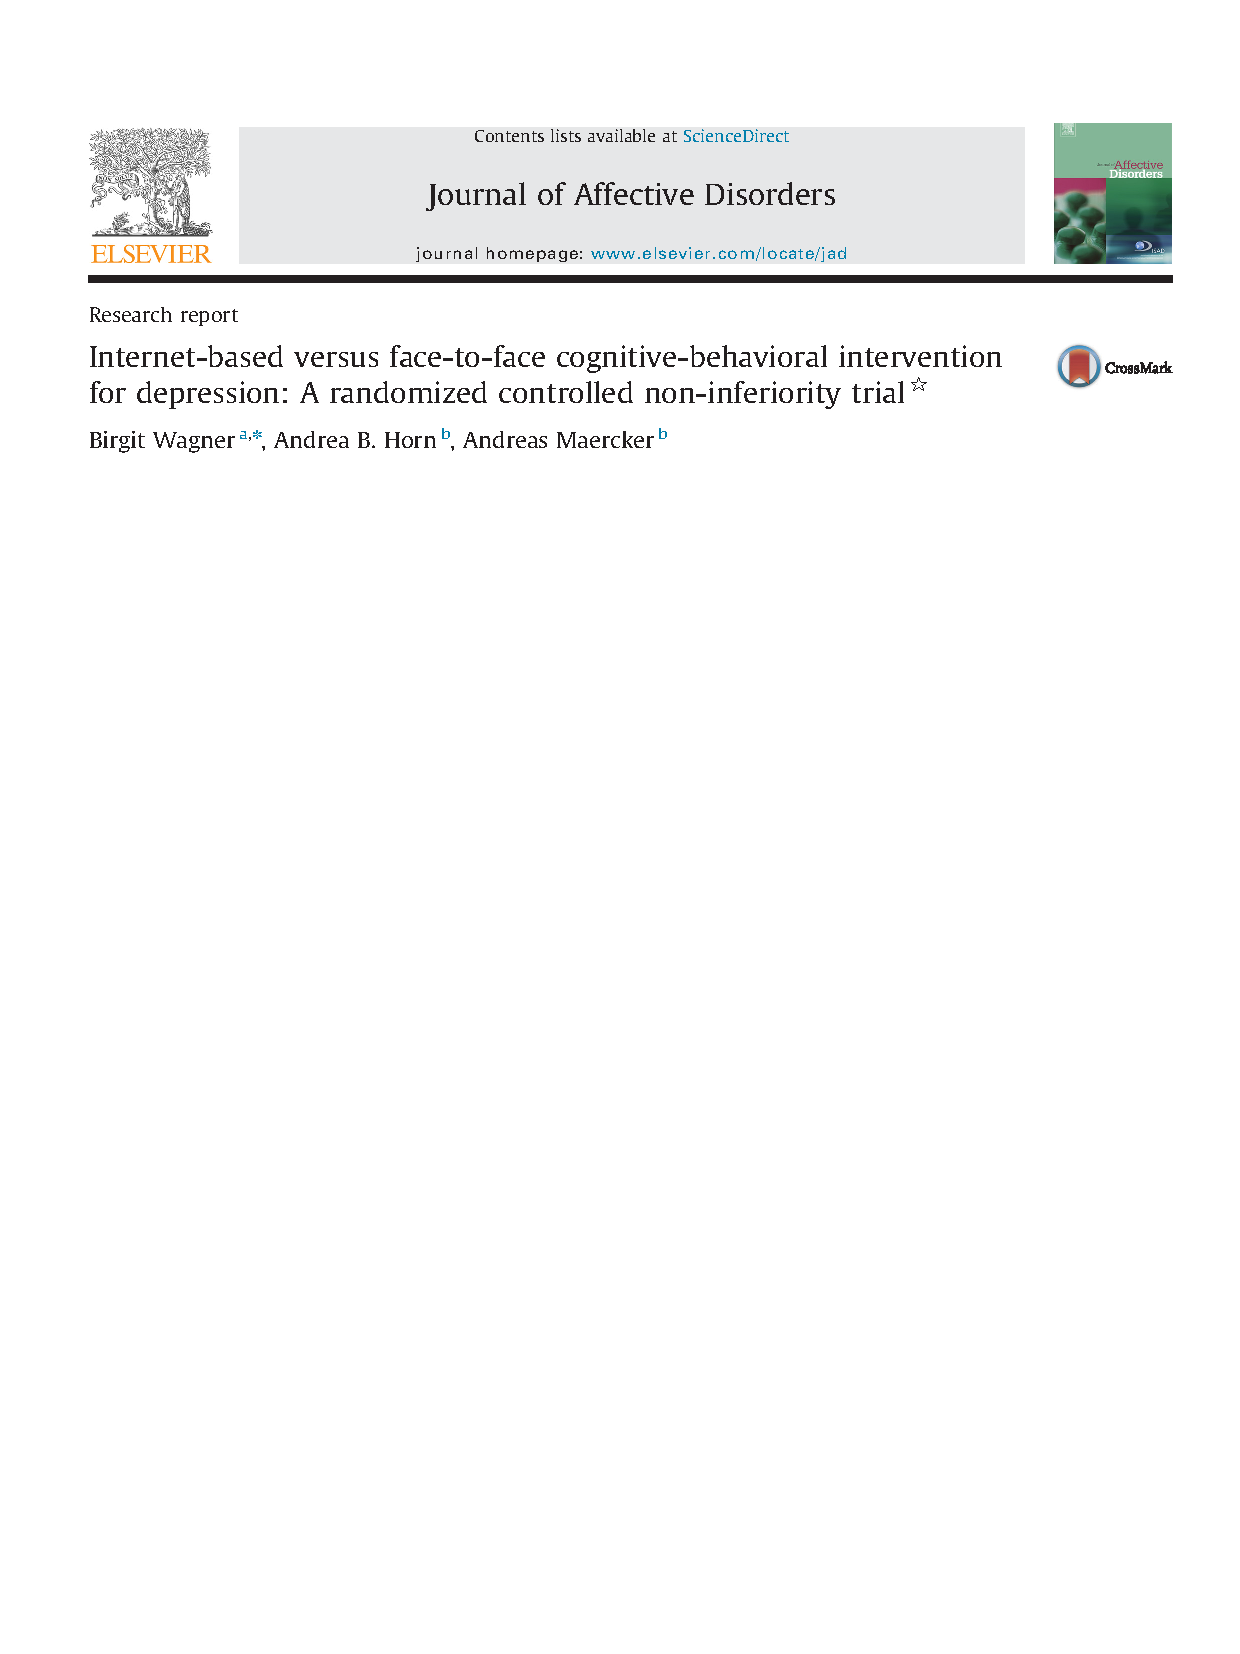
\includegraphics[width=0.5\linewidth]{8_Abbildungen/alm_8_article_title} \end{center}
\center

\textcolor{darkblue}{Participants}

\begin{center}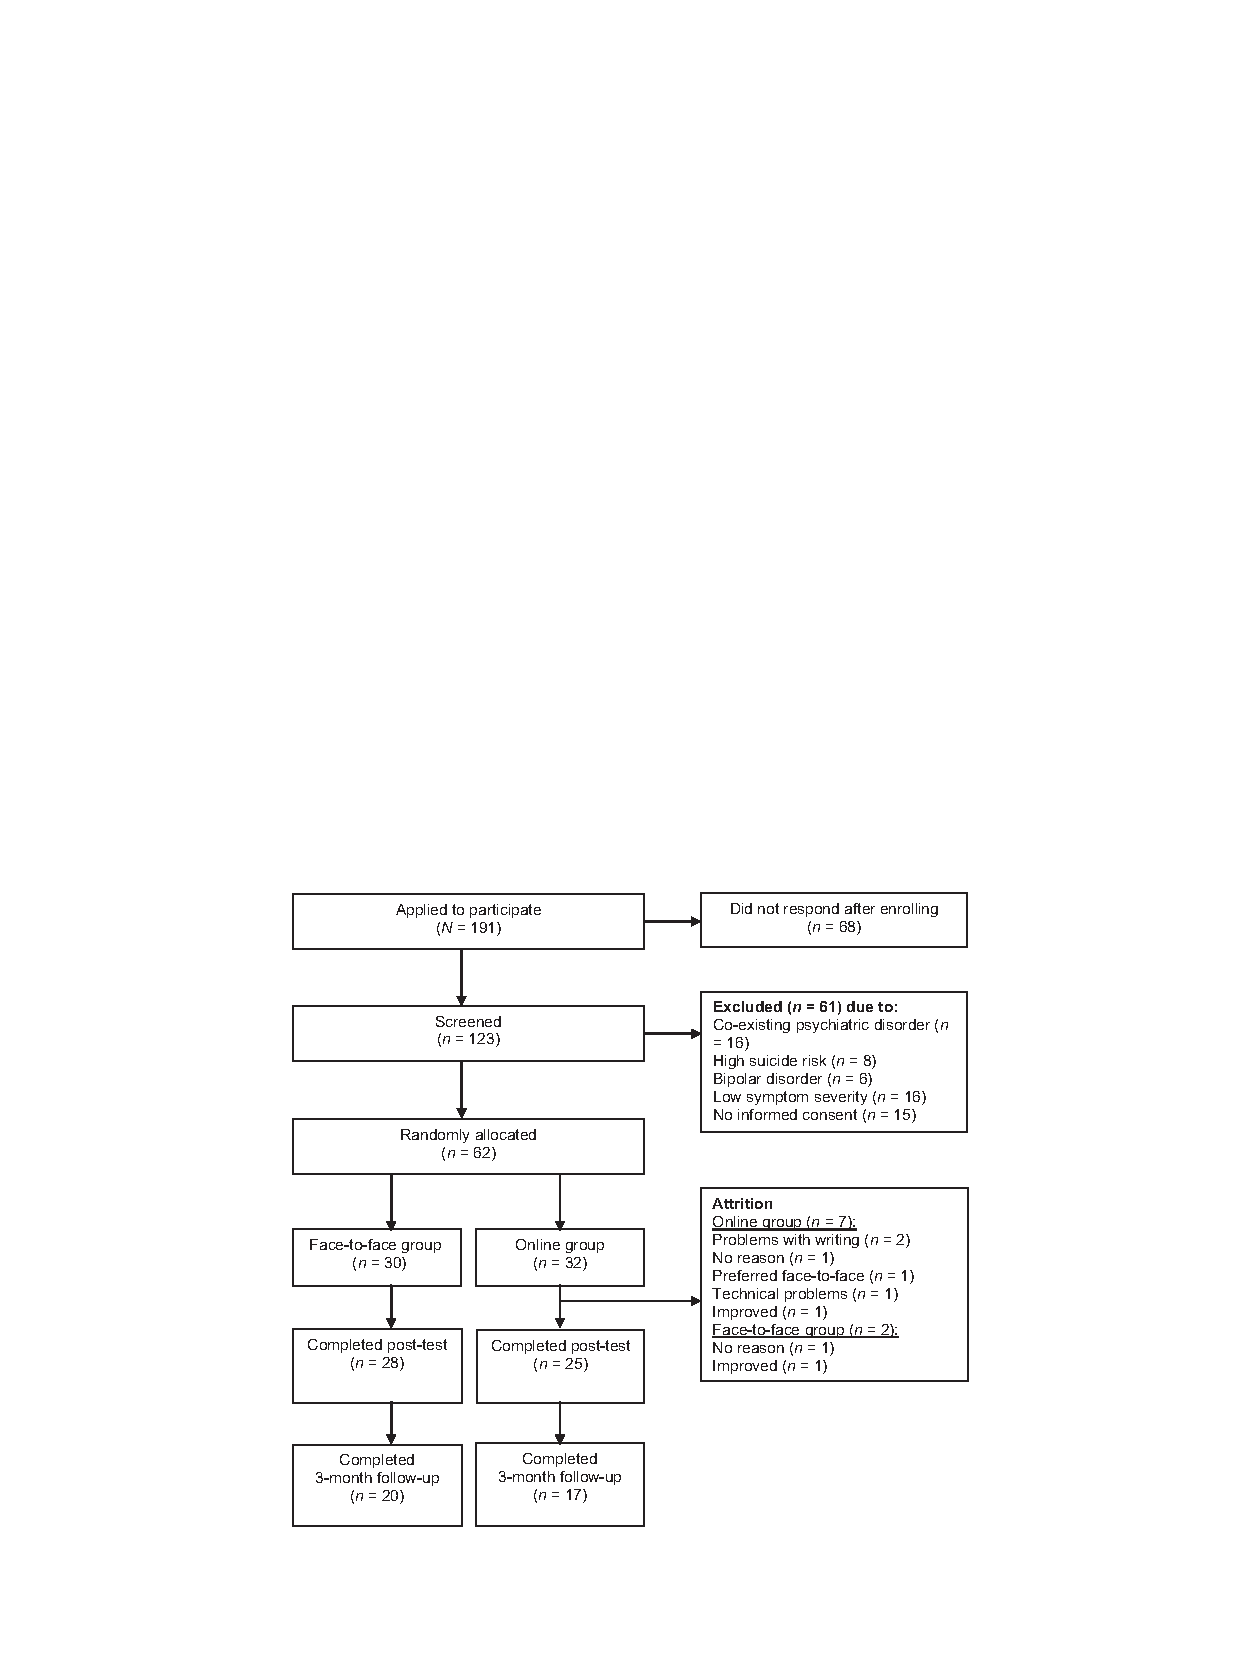
\includegraphics[width=0.5\linewidth]{8_Abbildungen/alm_8_article_participants} \end{center}
\flushright
\footnotesize

\emph{Wagner, Horn, and Maercker (2014)}
\end{frame}

\begin{frame}[t]{Anwendungskontext}
\protect\hypertarget{anwendungskontext-8}{}
\begin{center}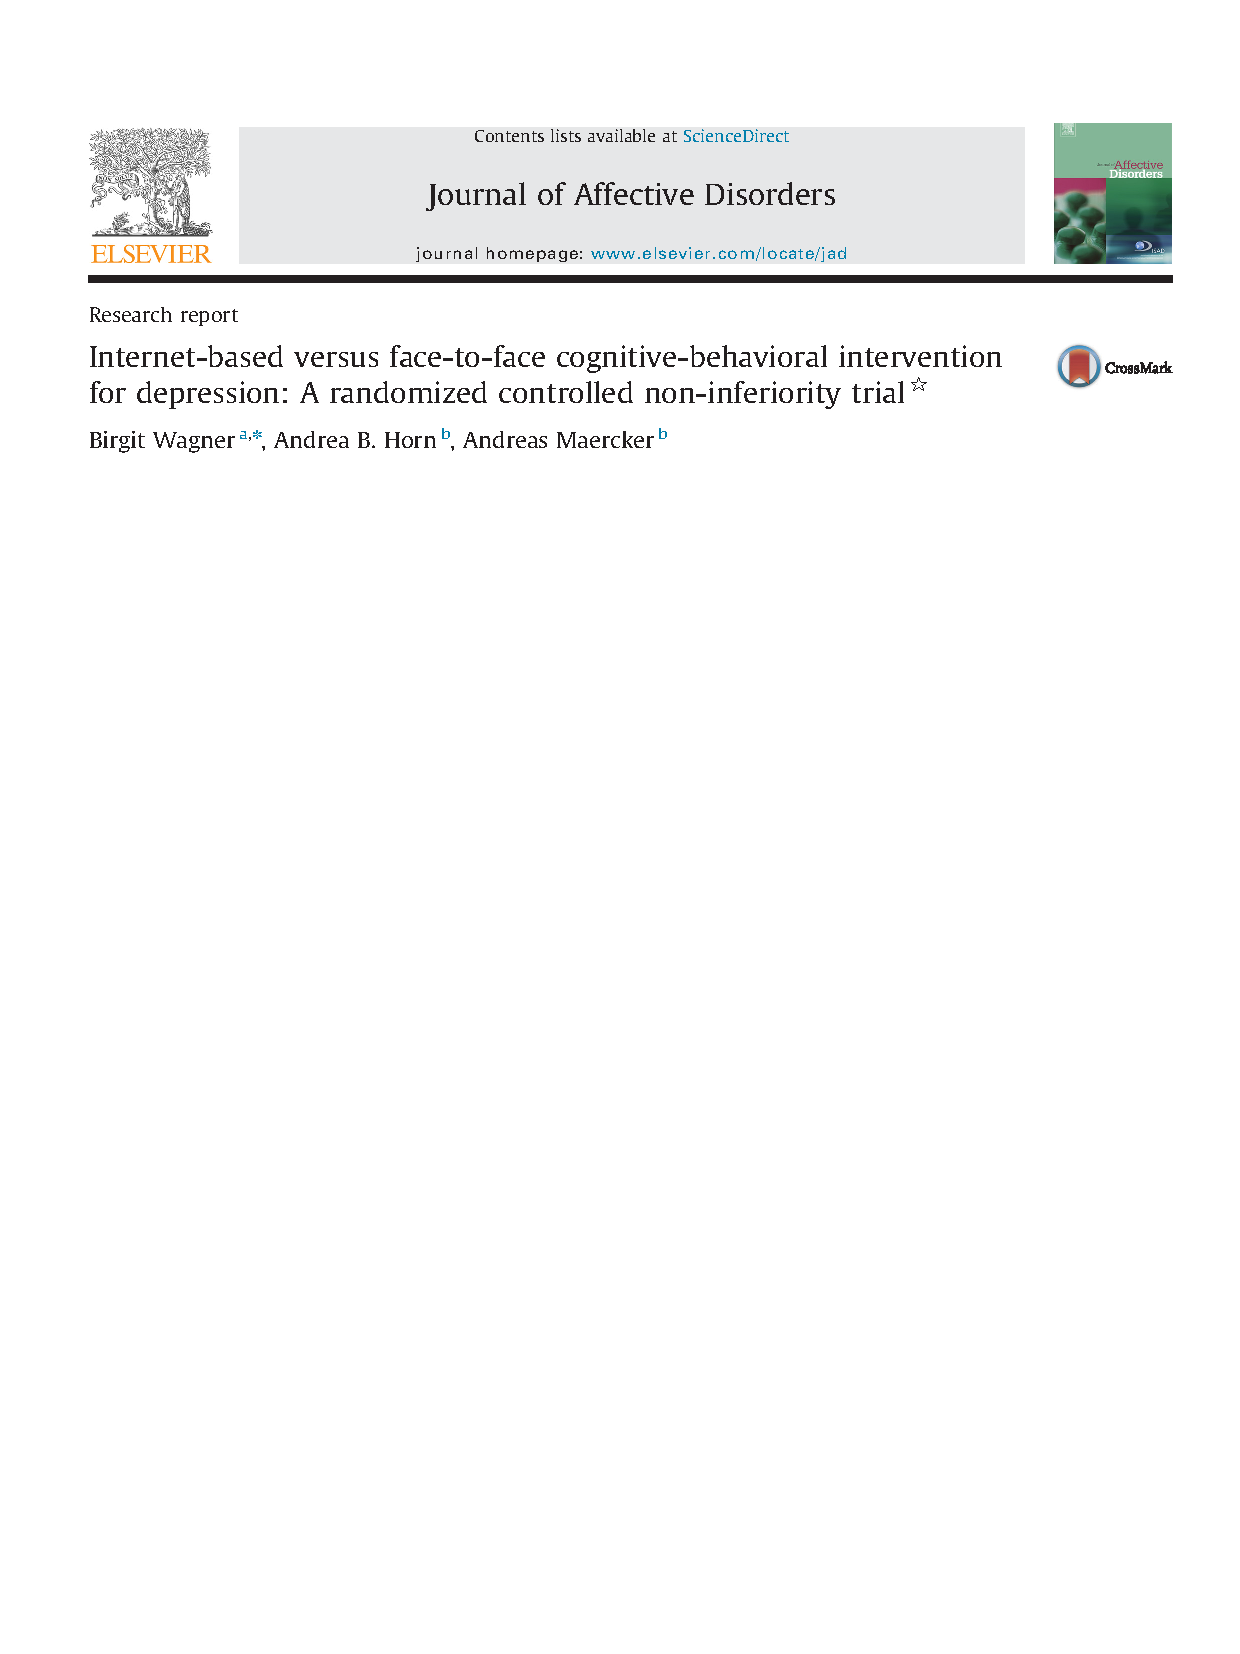
\includegraphics[width=0.5\linewidth]{8_Abbildungen/alm_8_article_title} \end{center}
\center

\textcolor{darkblue}{Demographics}

\begin{center}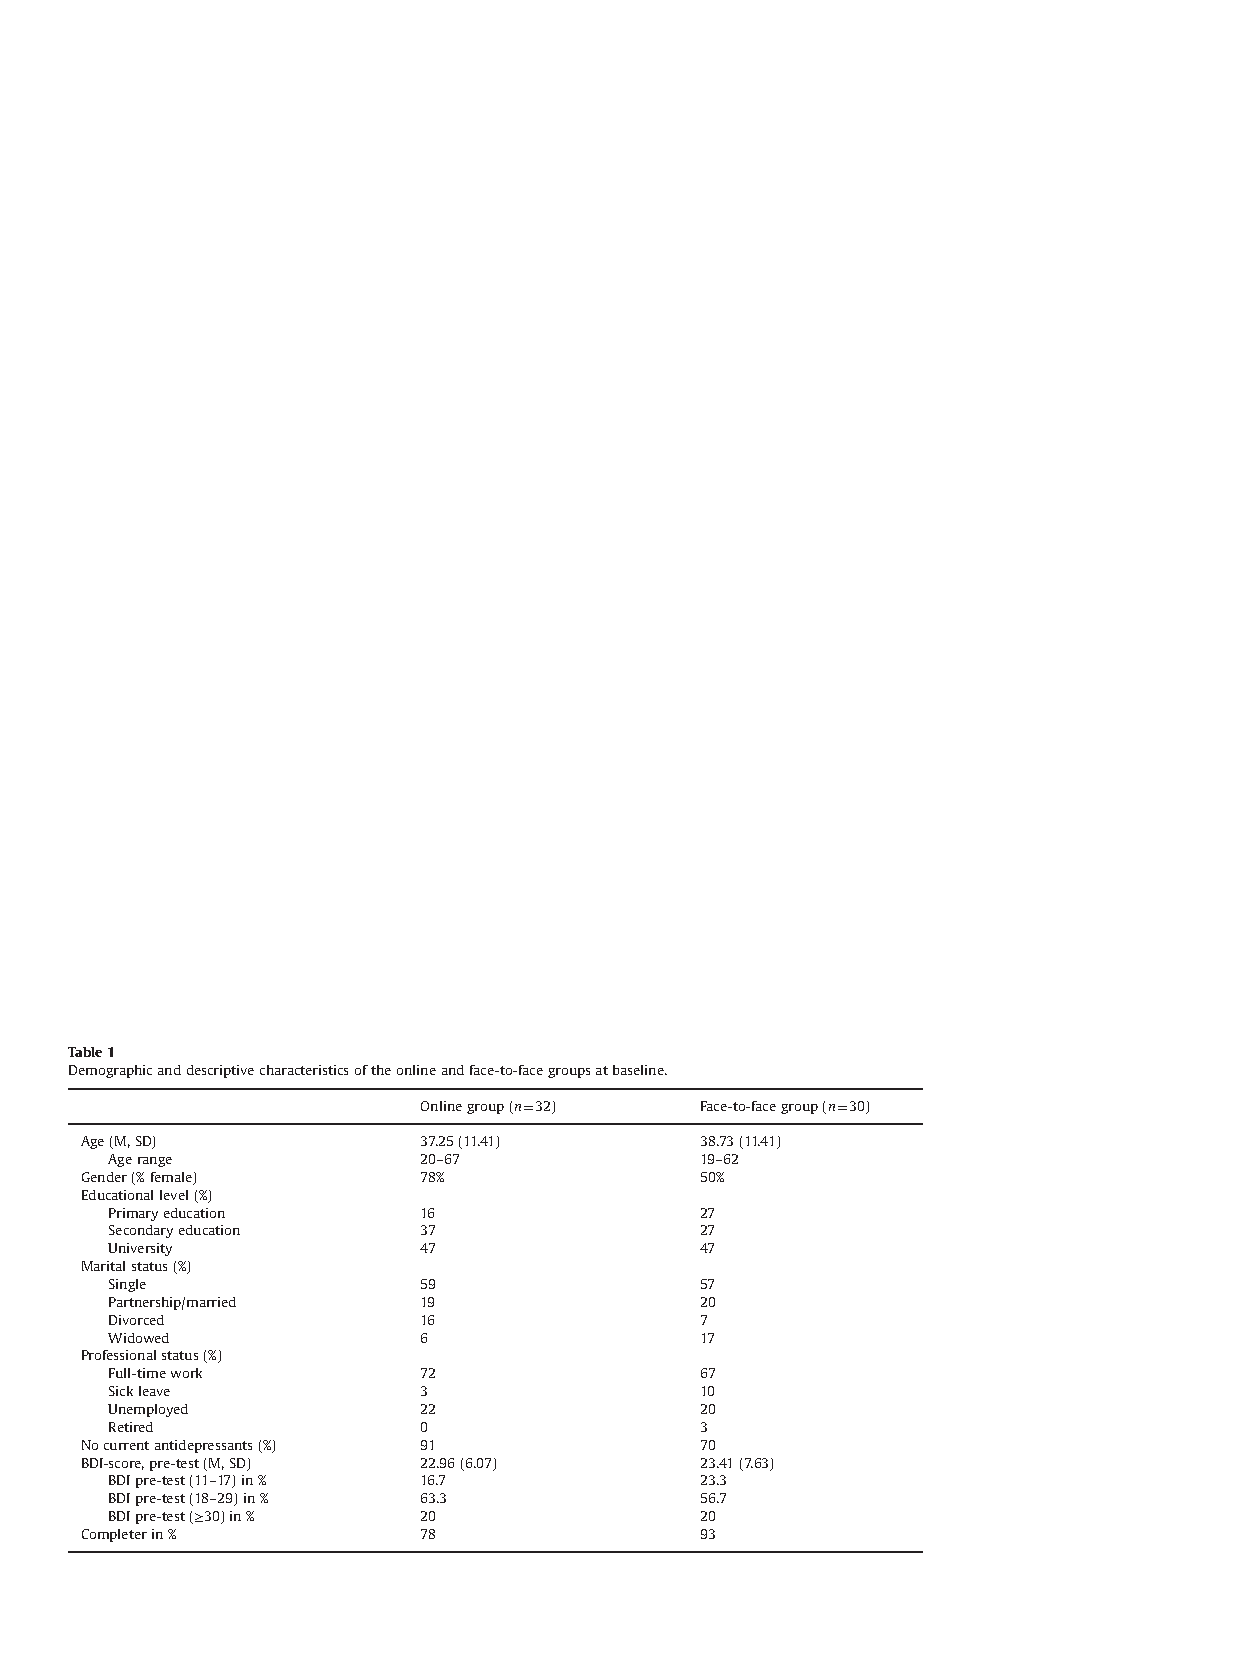
\includegraphics[width=0.7\linewidth]{8_Abbildungen/alm_8_article_demographics} \end{center}
\flushright
\footnotesize

\emph{Wagner, Horn, and Maercker (2014)}
\end{frame}

\begin{frame}[t]{Anwendungskontext}
\protect\hypertarget{anwendungskontext-9}{}
\begin{center}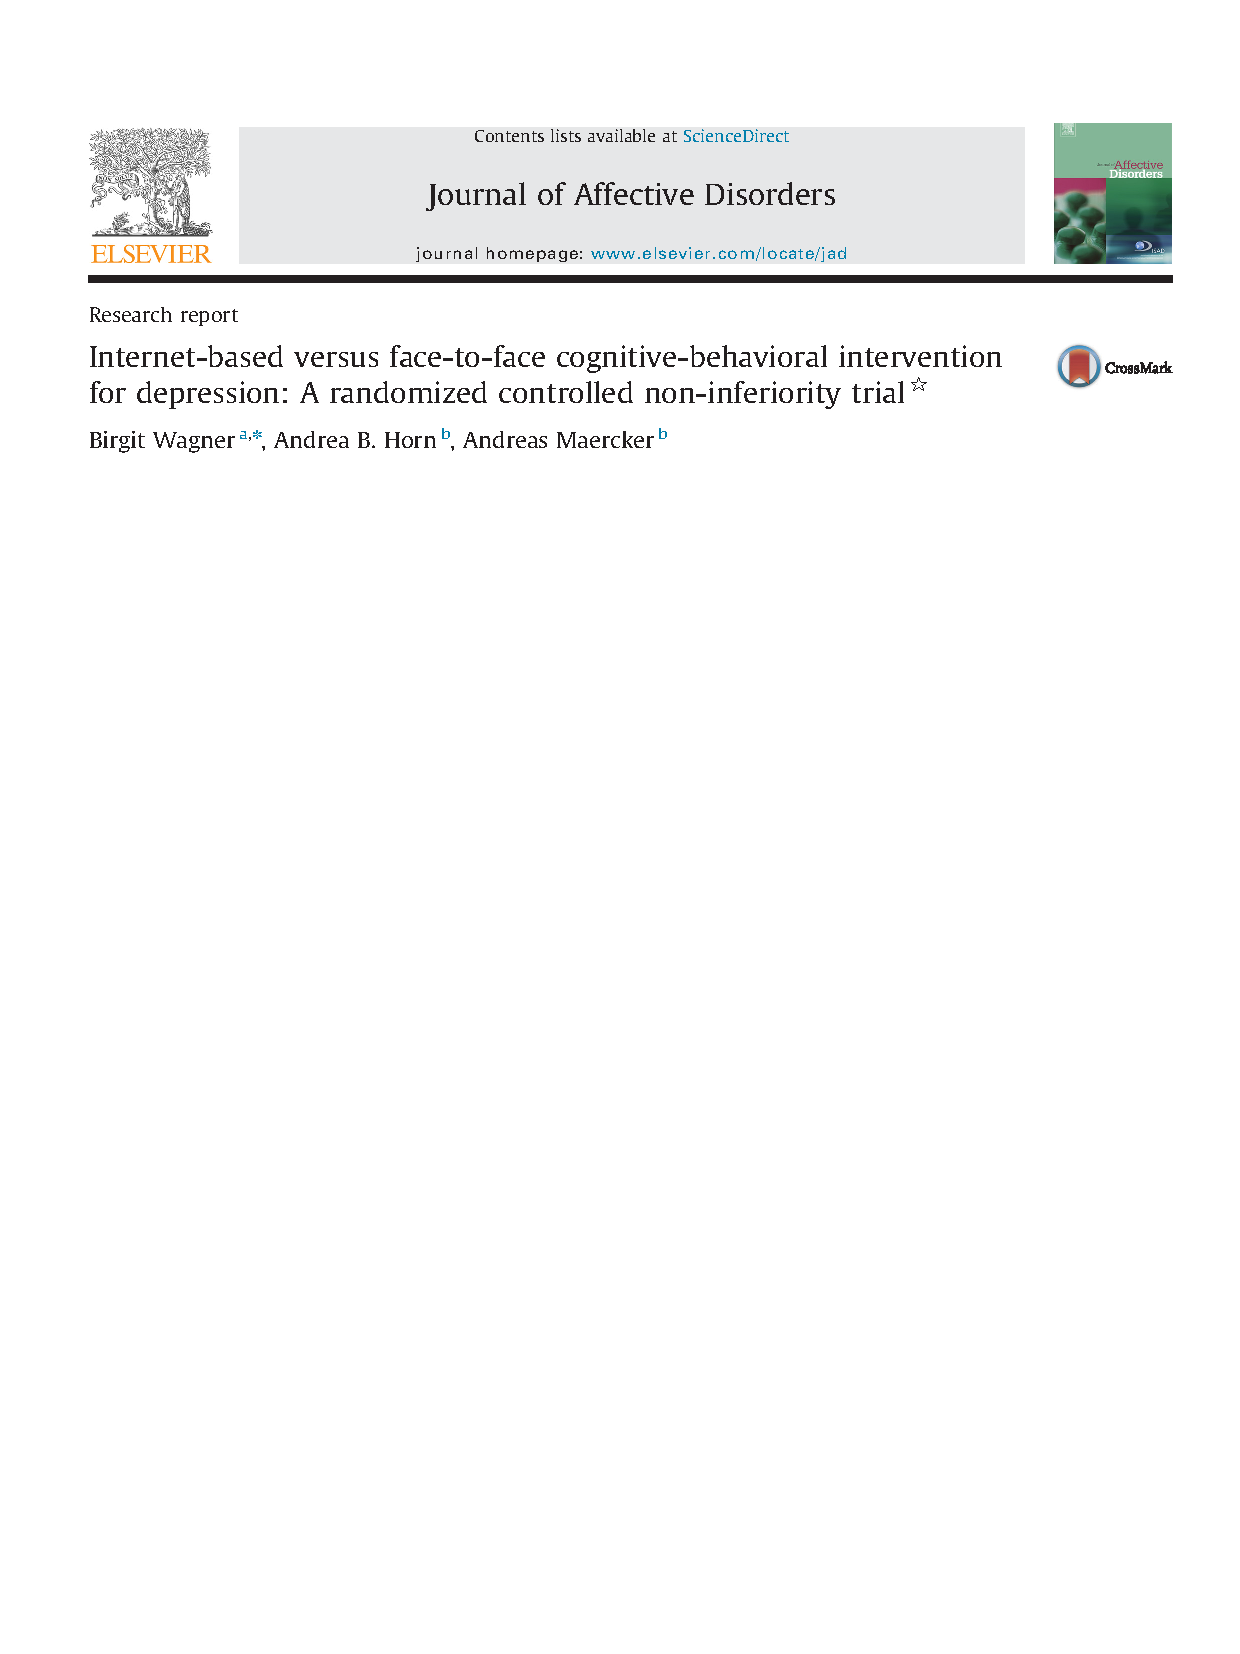
\includegraphics[width=0.5\linewidth]{8_Abbildungen/alm_8_article_title} \end{center}
\center

\textcolor{darkblue}{Procedure}

\begin{center}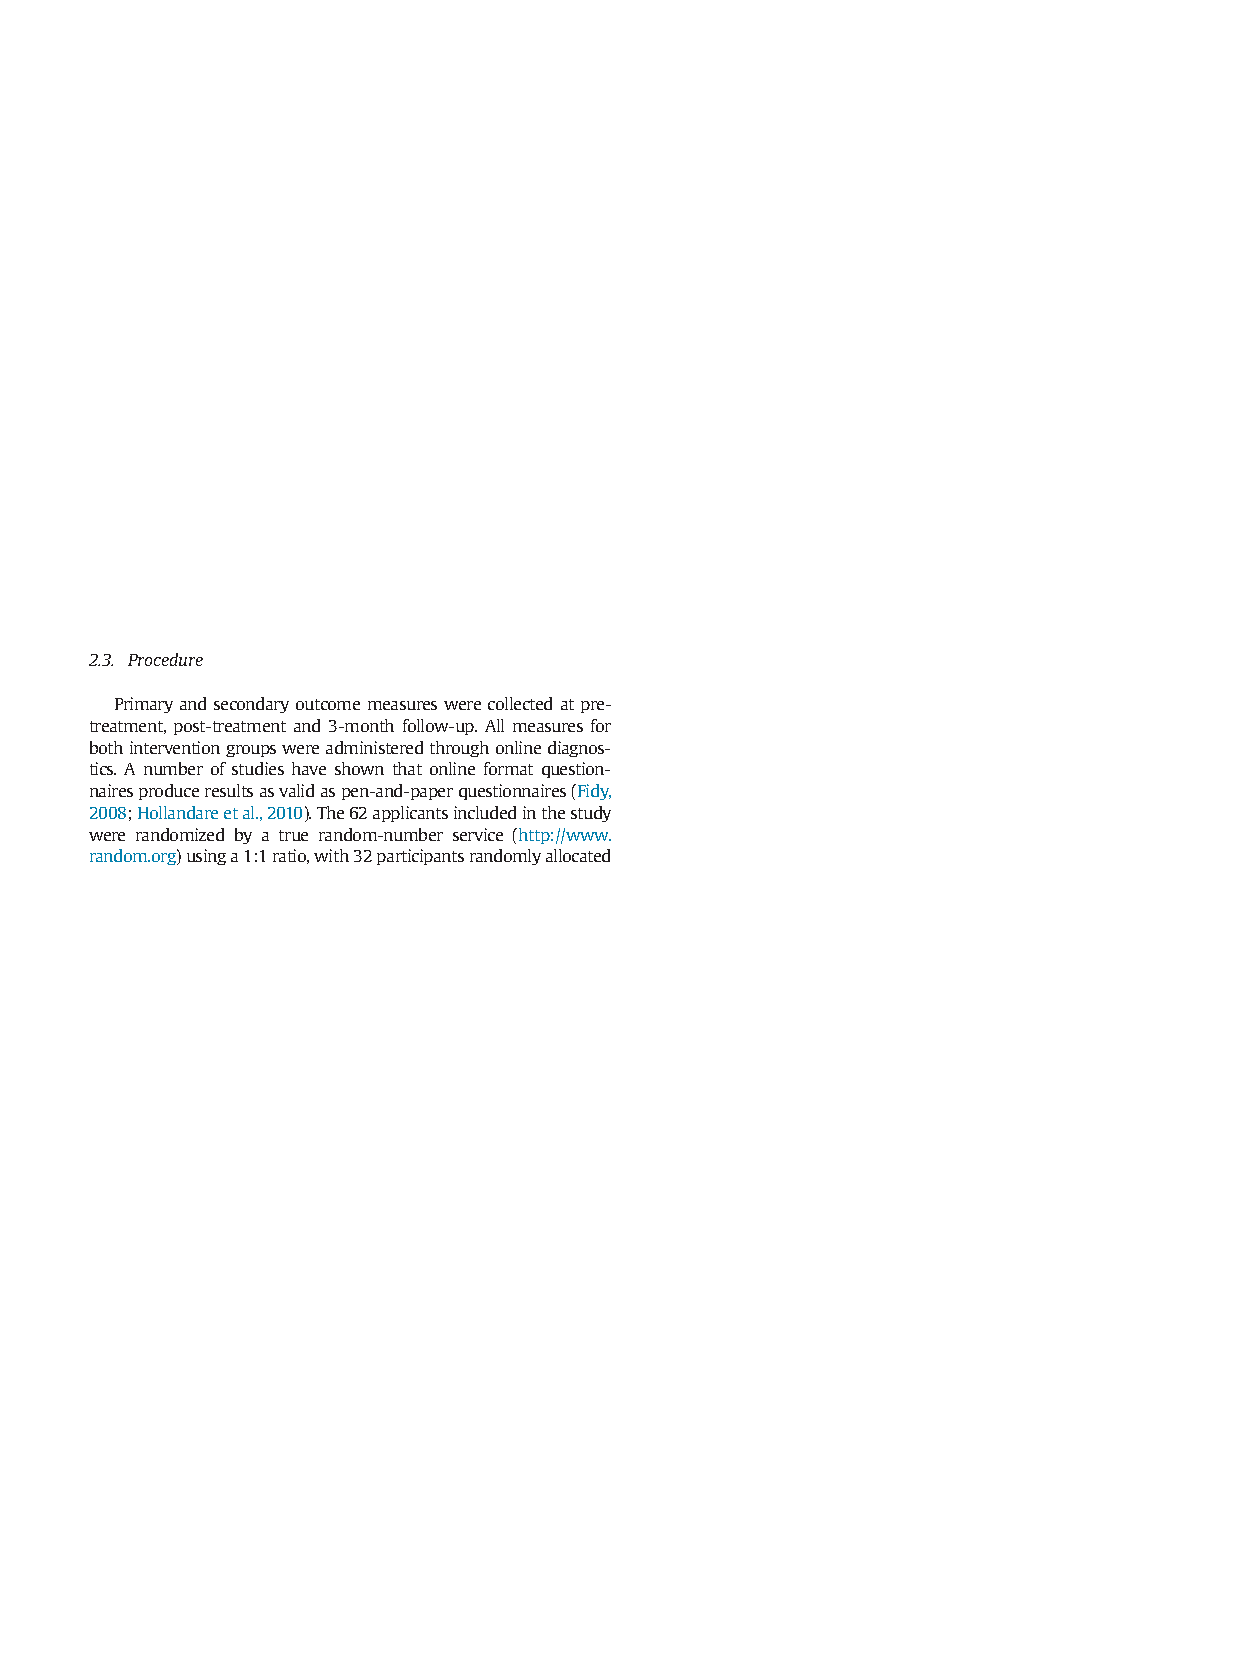
\includegraphics[width=0.5\linewidth]{8_Abbildungen/alm_8_article_procedure_1} \end{center}
\vspace{-3mm}

\begin{center}
\includegraphics[width=0.49\linewidth]{8_Abbildungen/alm_8_article_procedure_2} \end{center}
\vfill
\flushright
\footnotesize

\emph{Wagner, Horn, and Maercker (2014)}
\end{frame}

\begin{frame}[t]{Anwendungskontext}
\protect\hypertarget{anwendungskontext-10}{}
\begin{center}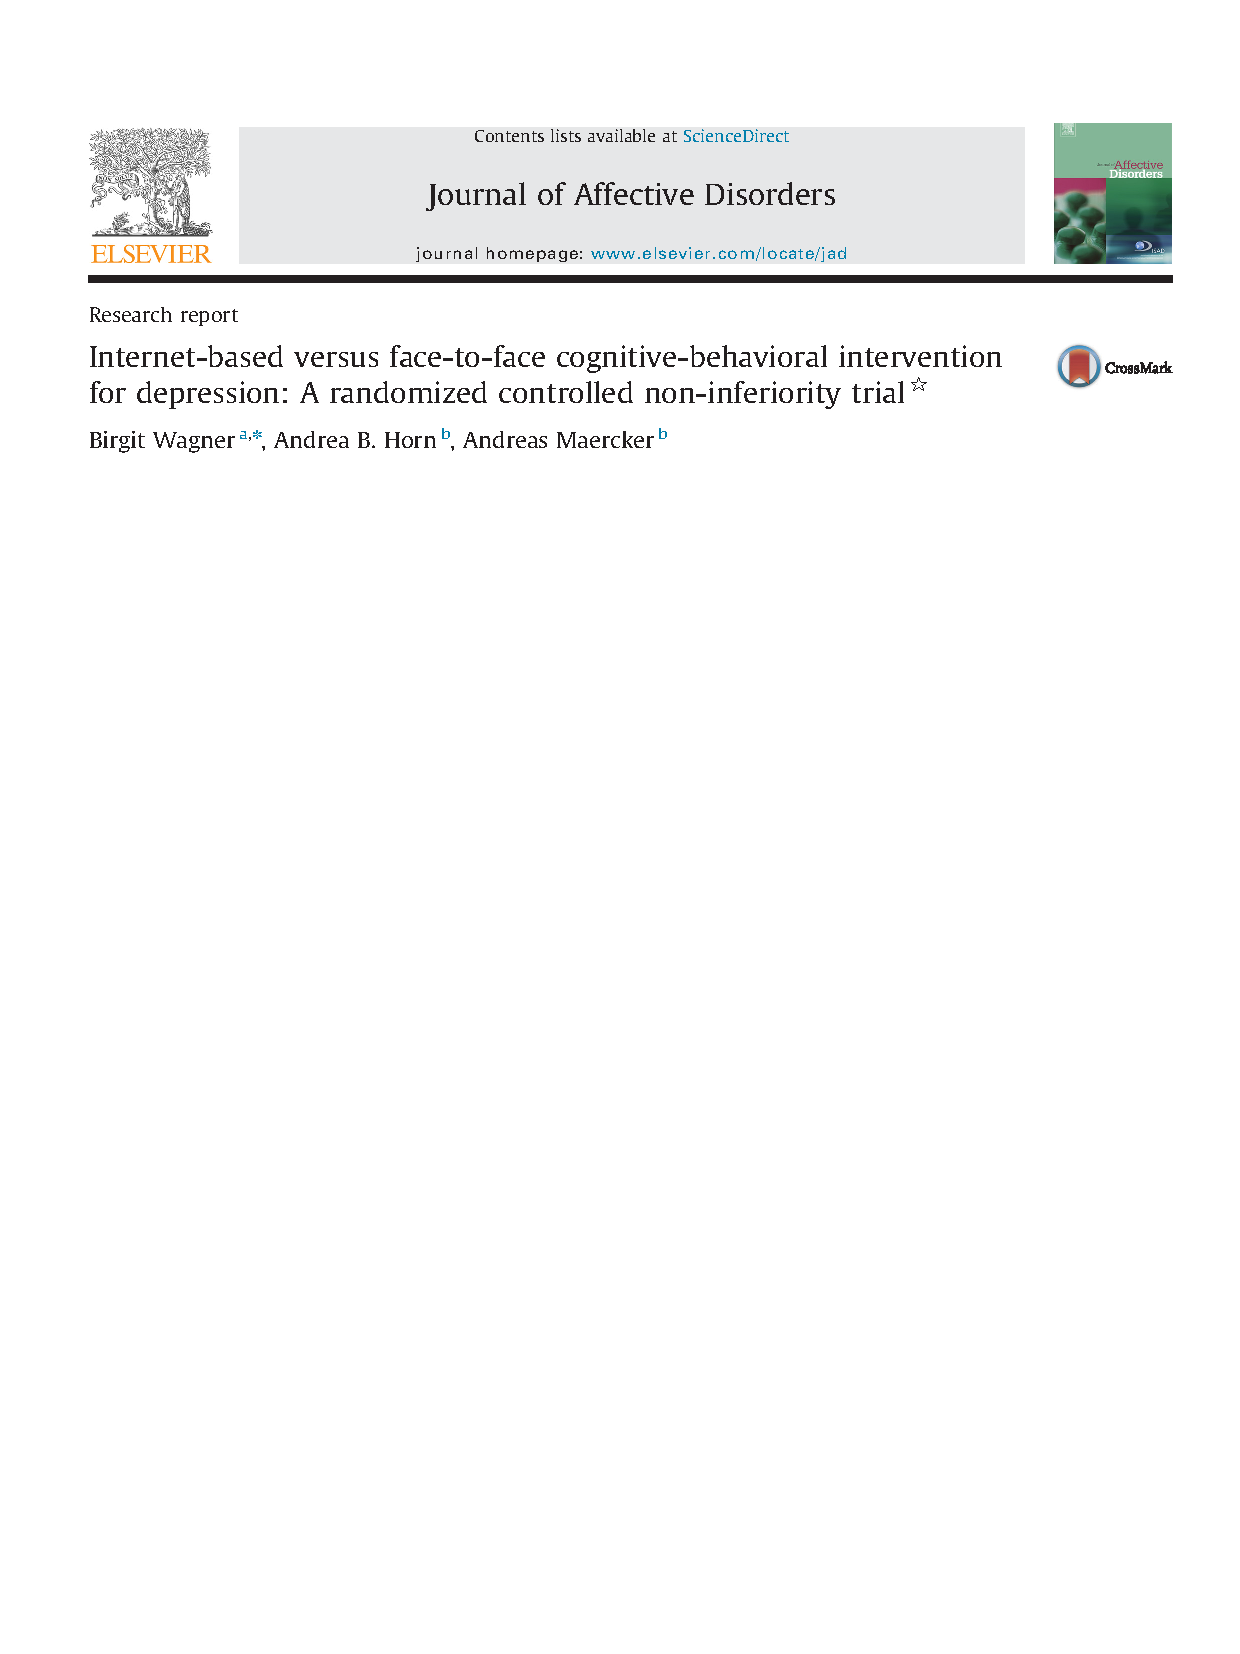
\includegraphics[width=0.5\linewidth]{8_Abbildungen/alm_8_article_title} \end{center}
\center

\textcolor{darkblue}{Interventions}

\begin{center}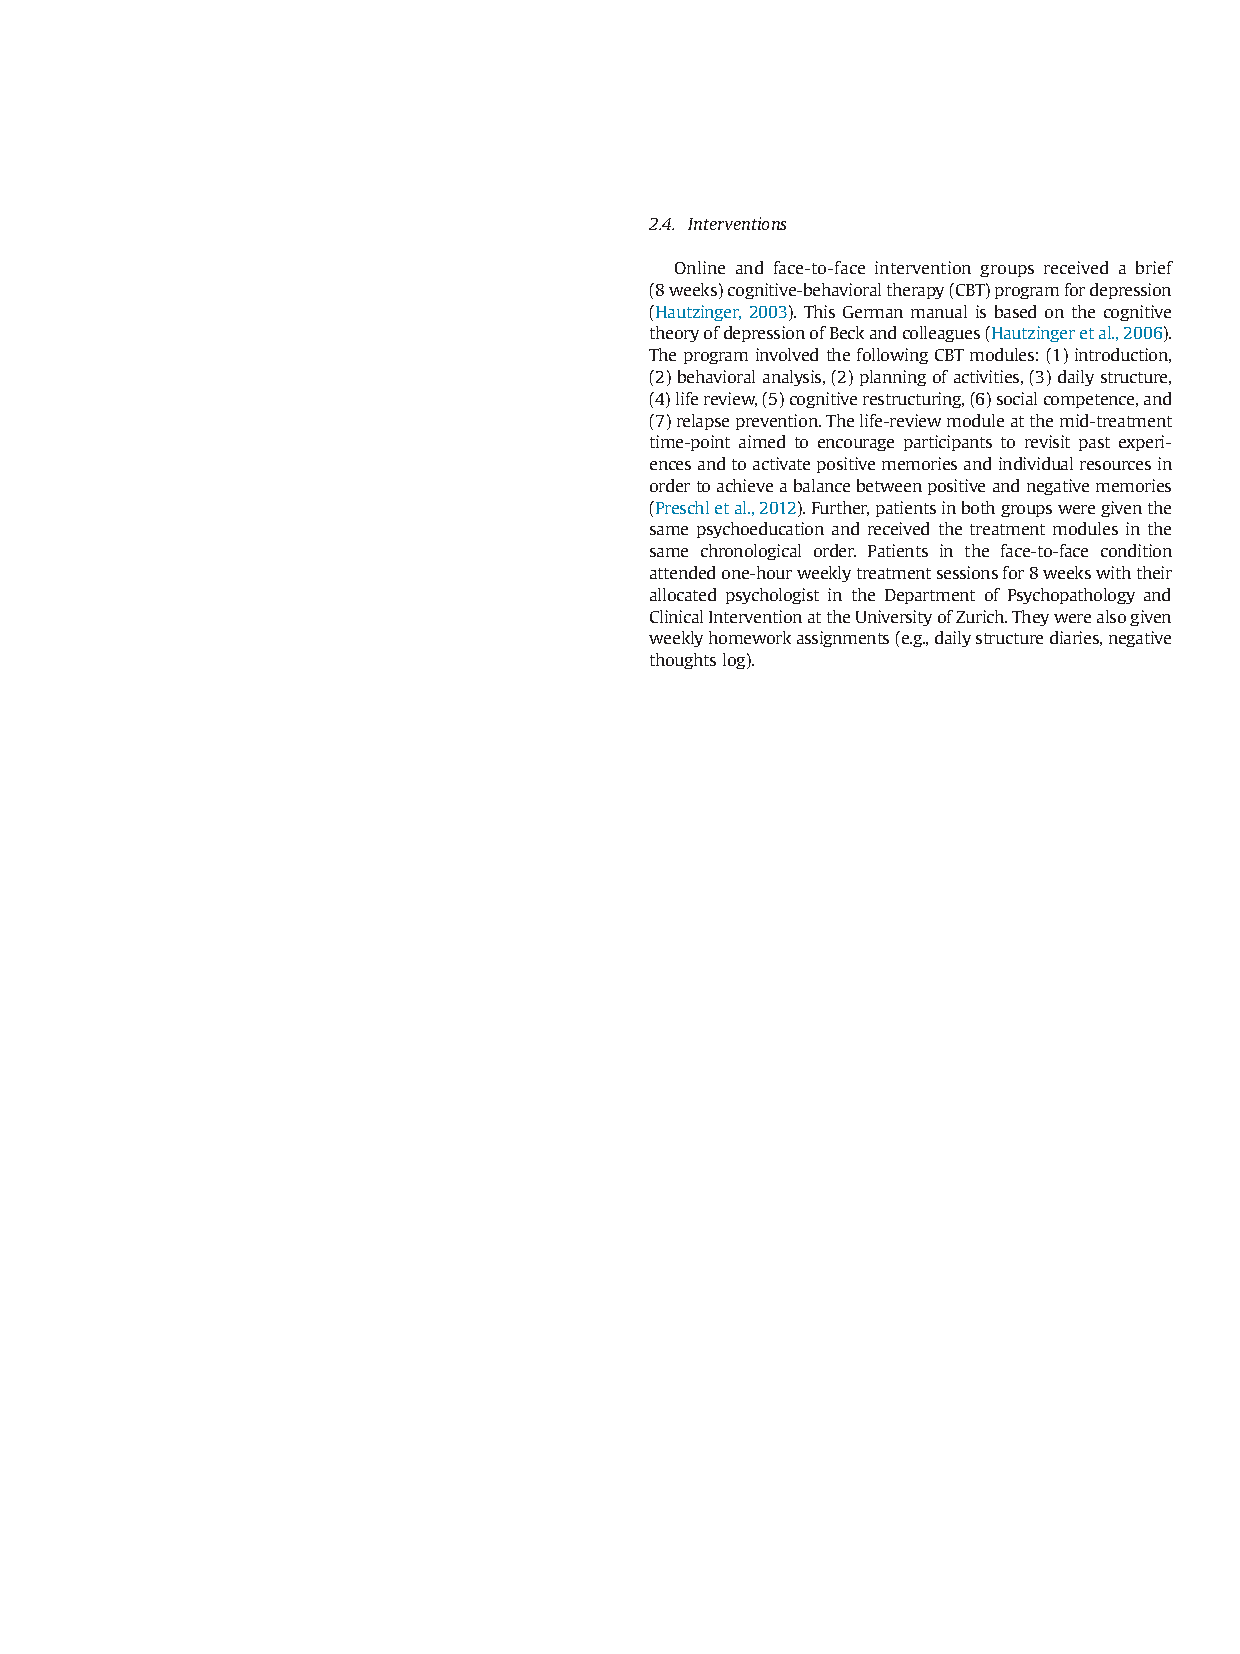
\includegraphics[width=0.3\linewidth]{8_Abbildungen/alm_8_article_intervention_1} \end{center}
\vspace{-2mm}

\begin{center}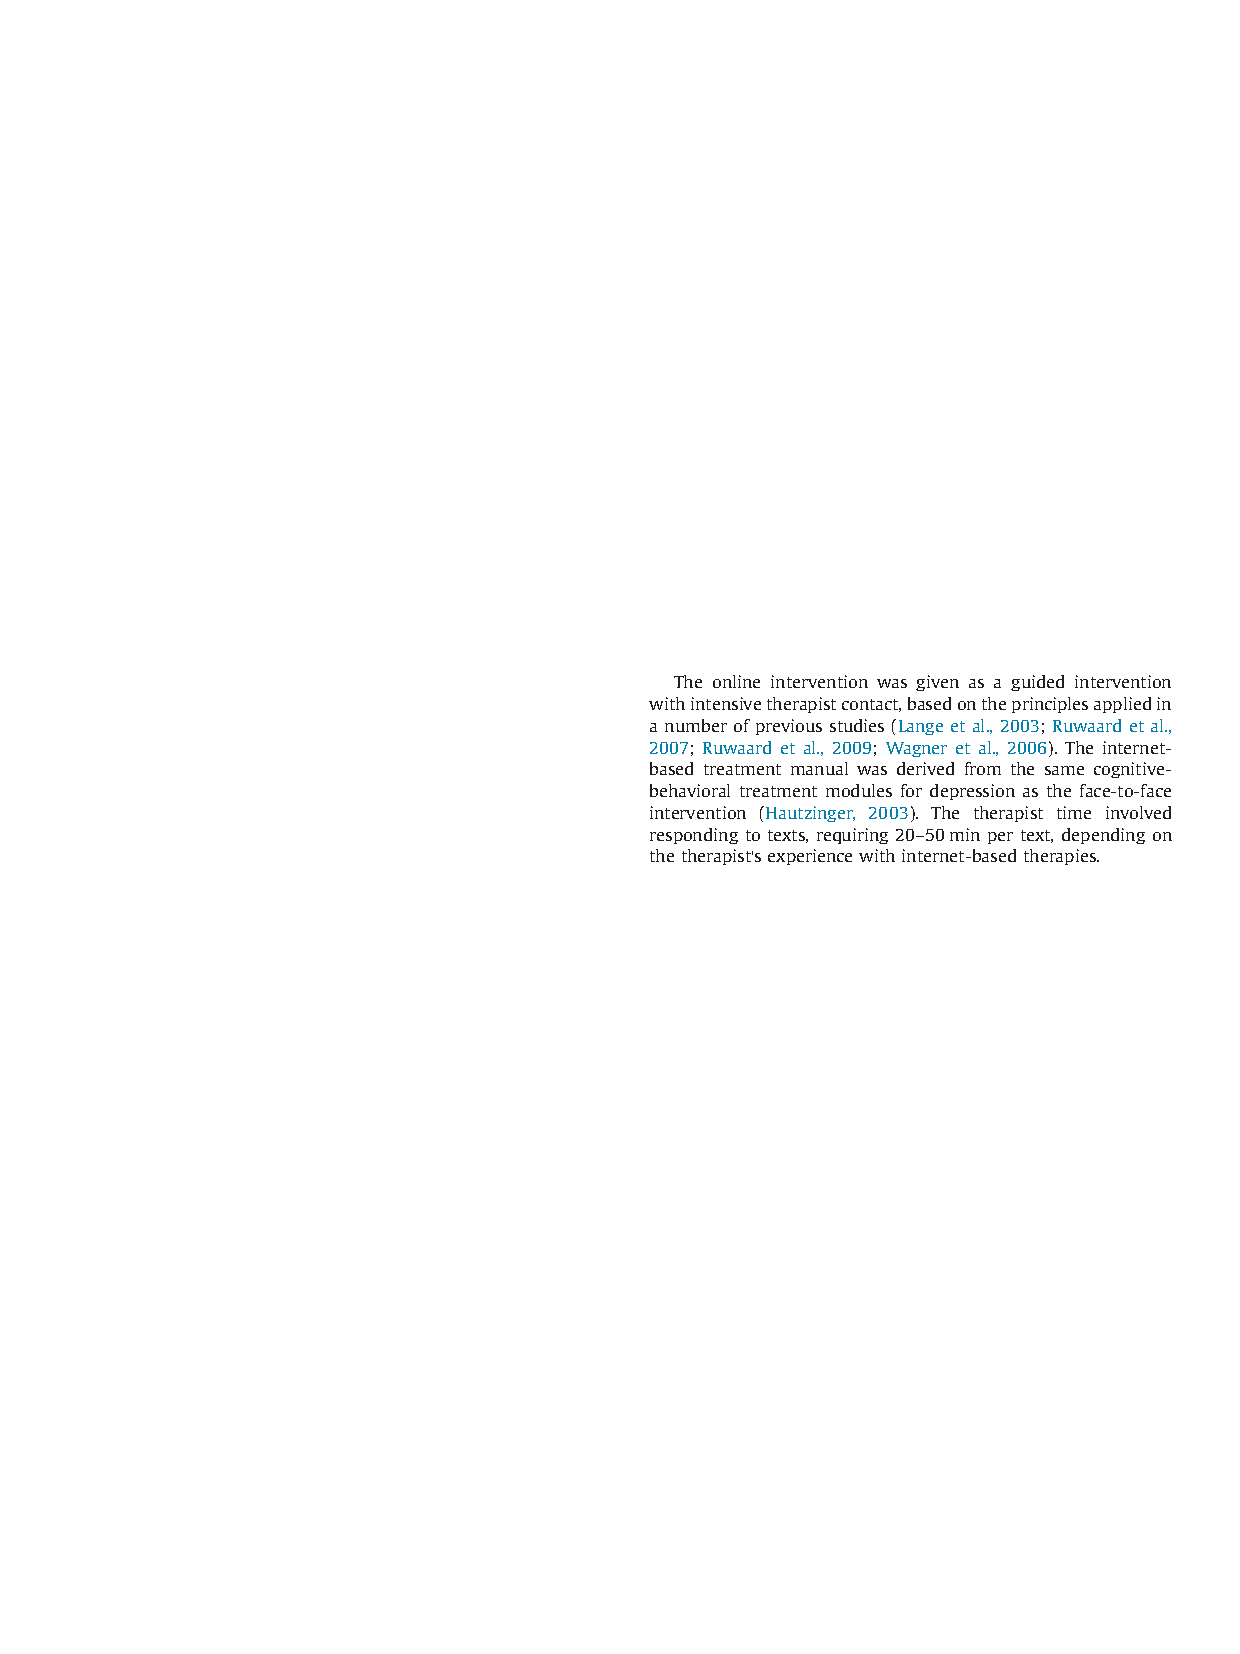
\includegraphics[width=0.3\linewidth]{8_Abbildungen/alm_8_article_intervention_2} \end{center}
\vspace{-2mm}

\begin{center}
\includegraphics[width=0.3\linewidth]{8_Abbildungen/alm_8_article_intervention_3} \end{center}
\flushright
\footnotesize

\emph{Wagner, Horn, and Maercker (2014)}
\end{frame}

\begin{frame}[t]{Anwendungskontext}
\protect\hypertarget{anwendungskontext-11}{}
\begin{center}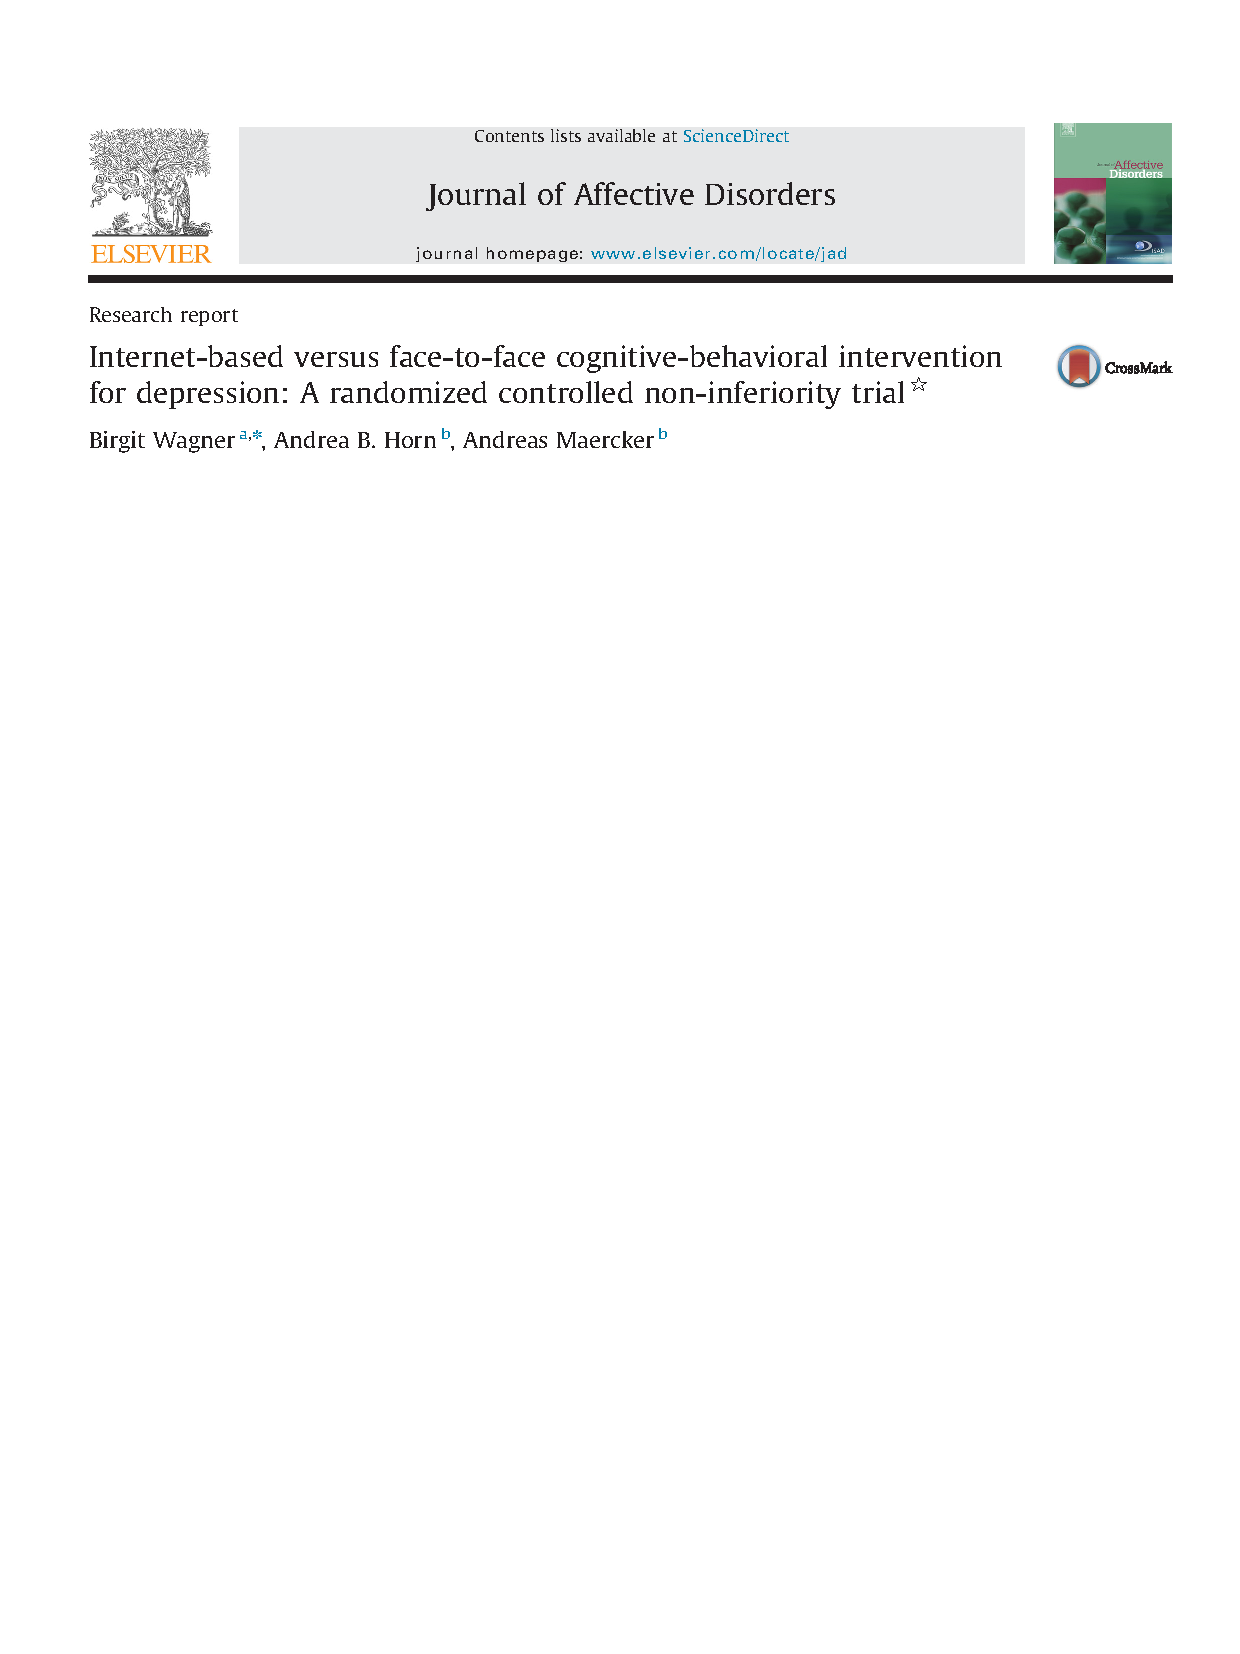
\includegraphics[width=0.5\linewidth]{8_Abbildungen/alm_8_article_title} \end{center}
\center

\textcolor{darkblue}{Outcome measure (Abhängige Variable)}

\begin{center}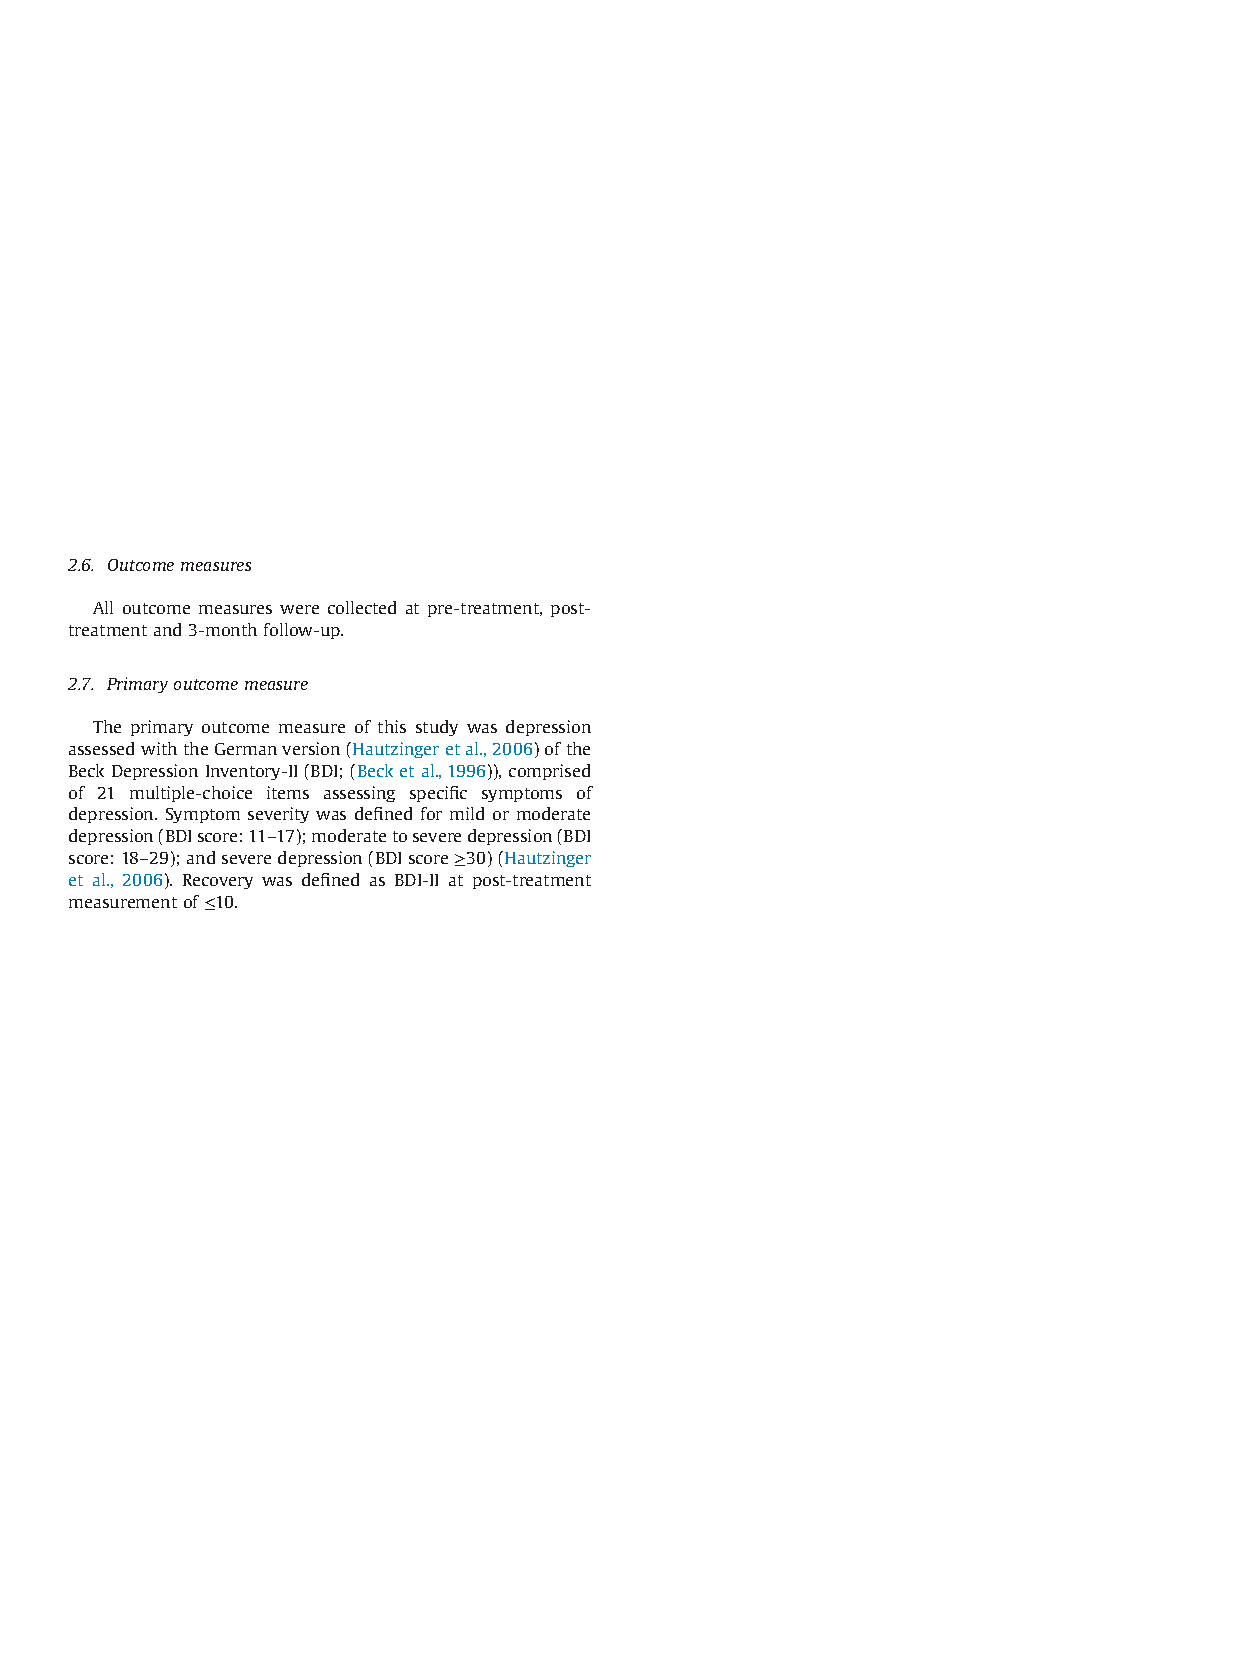
\includegraphics[width=0.5\linewidth]{8_Abbildungen/alm_8_article_outcome_measures} \end{center}
\flushright
\footnotesize

\emph{Wagner, Horn, and Maercker (2014)}
\end{frame}

\begin{frame}[t]{Anwendungskontext}
\protect\hypertarget{anwendungskontext-12}{}
\begin{center}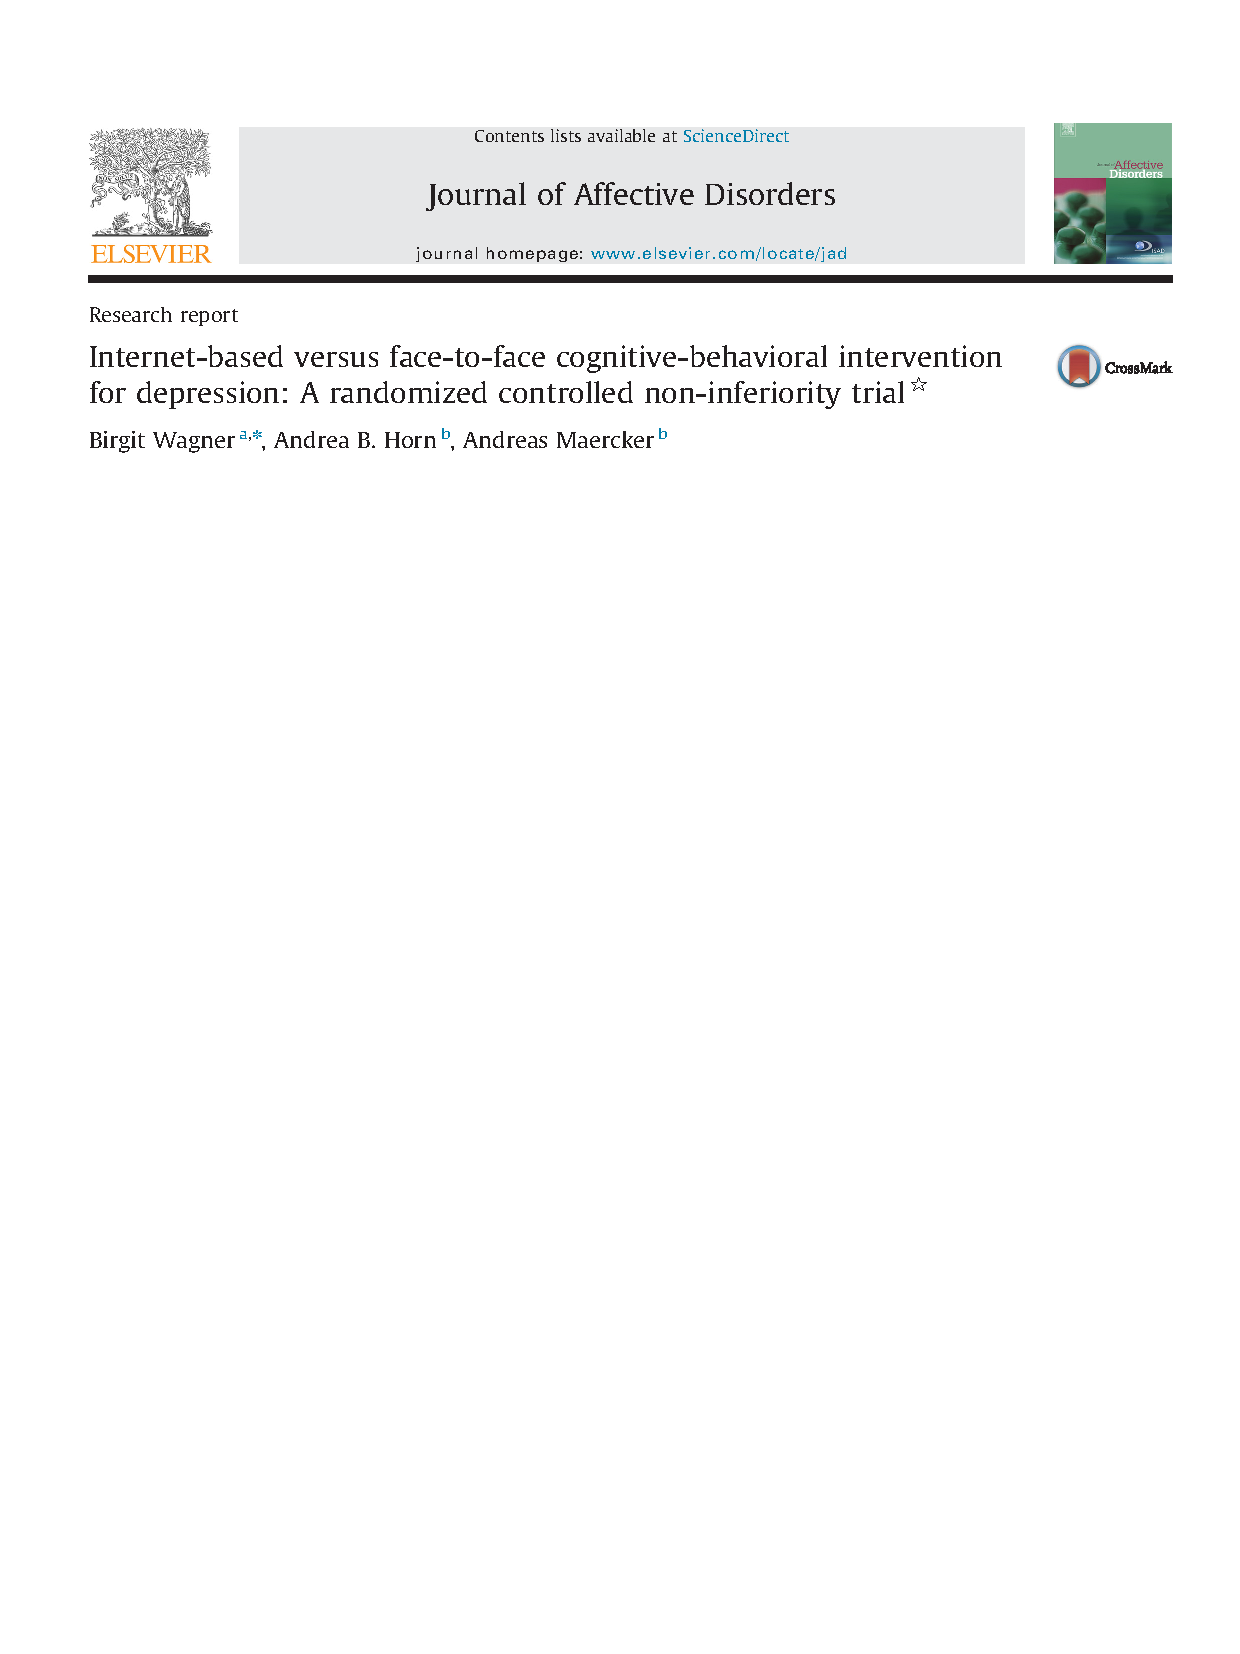
\includegraphics[width=0.5\linewidth]{8_Abbildungen/alm_8_article_title} \end{center}
\center

\textcolor{darkblue}{Results}

\begin{center}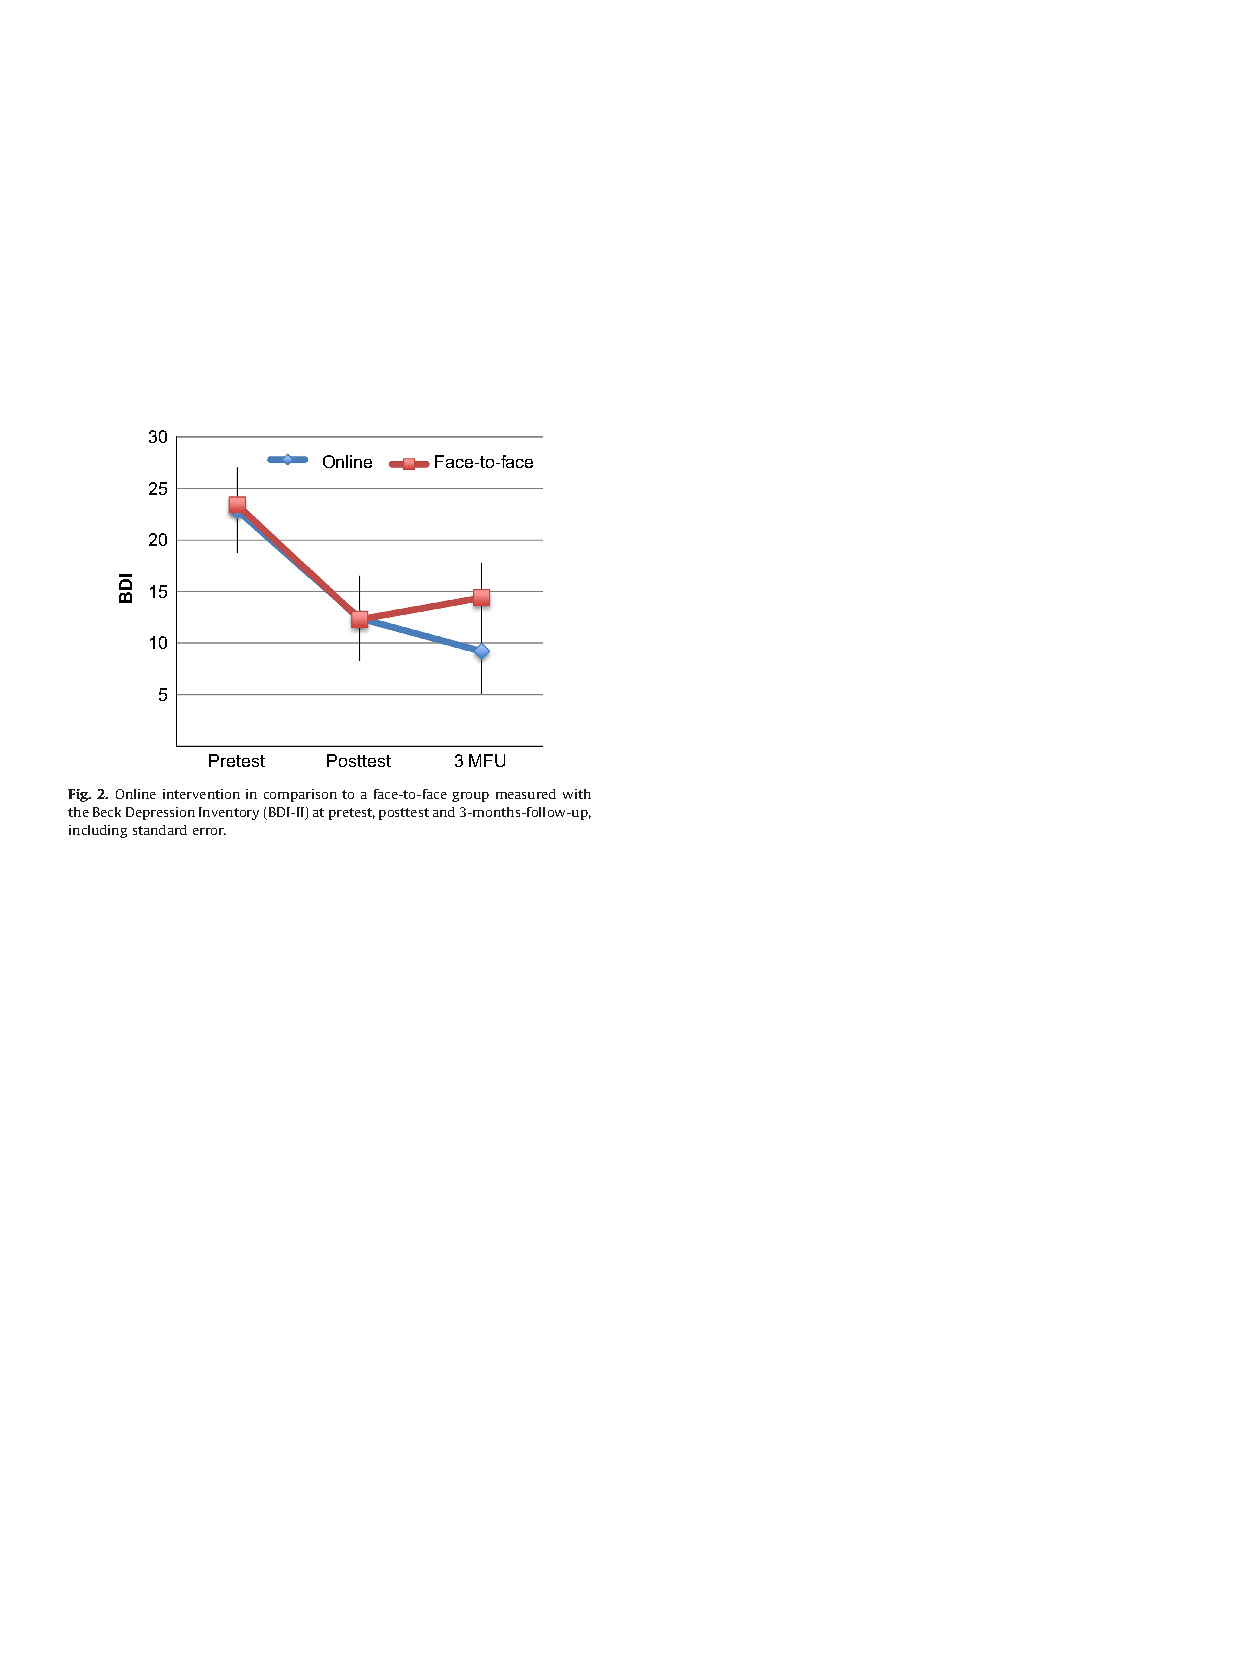
\includegraphics[width=0.55\linewidth]{8_Abbildungen/alm_8_article_results} \end{center}
\flushright
\footnotesize

\emph{Wagner, Horn, and Maercker (2014)}
\end{frame}

\begin{frame}[t]{Anwendungskontext}
\protect\hypertarget{anwendungskontext-13}{}
\begin{center}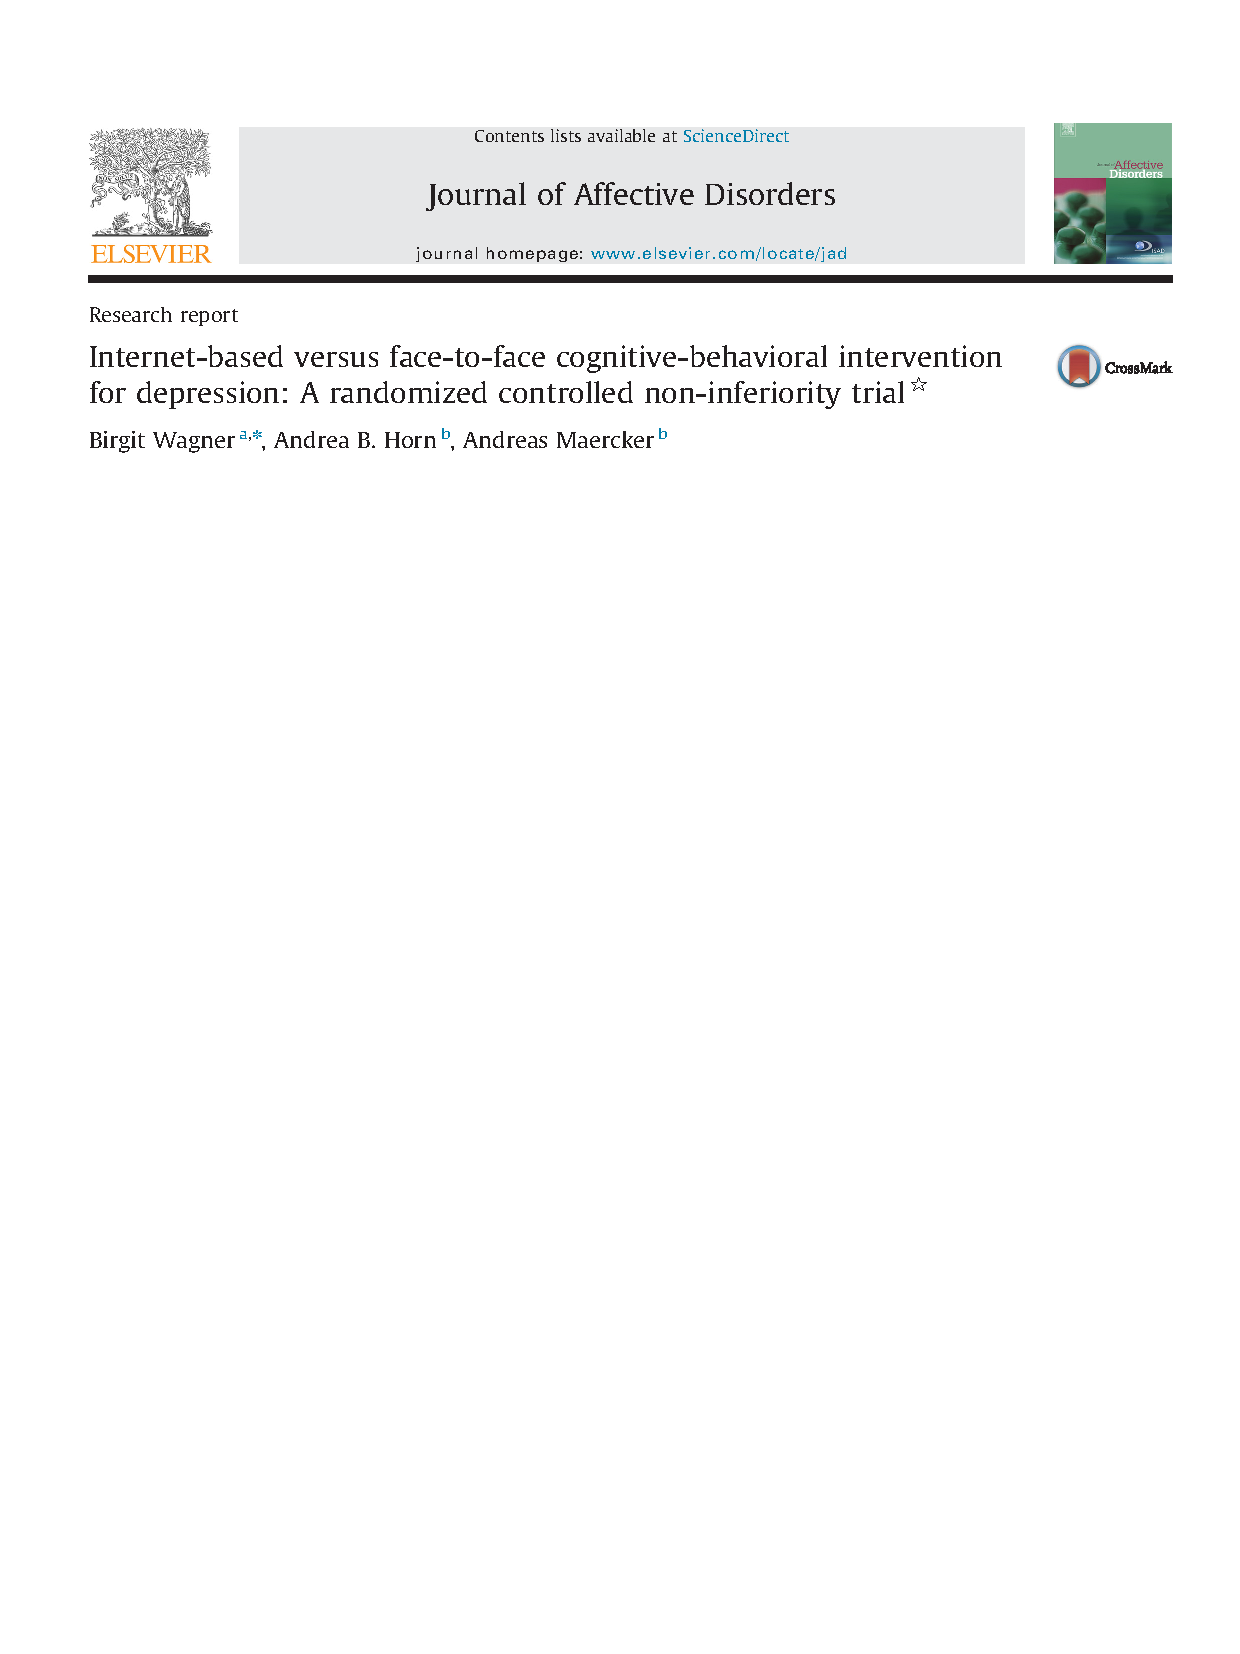
\includegraphics[width=0.5\linewidth]{8_Abbildungen/alm_8_article_title} \end{center}
\center

\textcolor{darkblue}{Discussion}

\begin{center}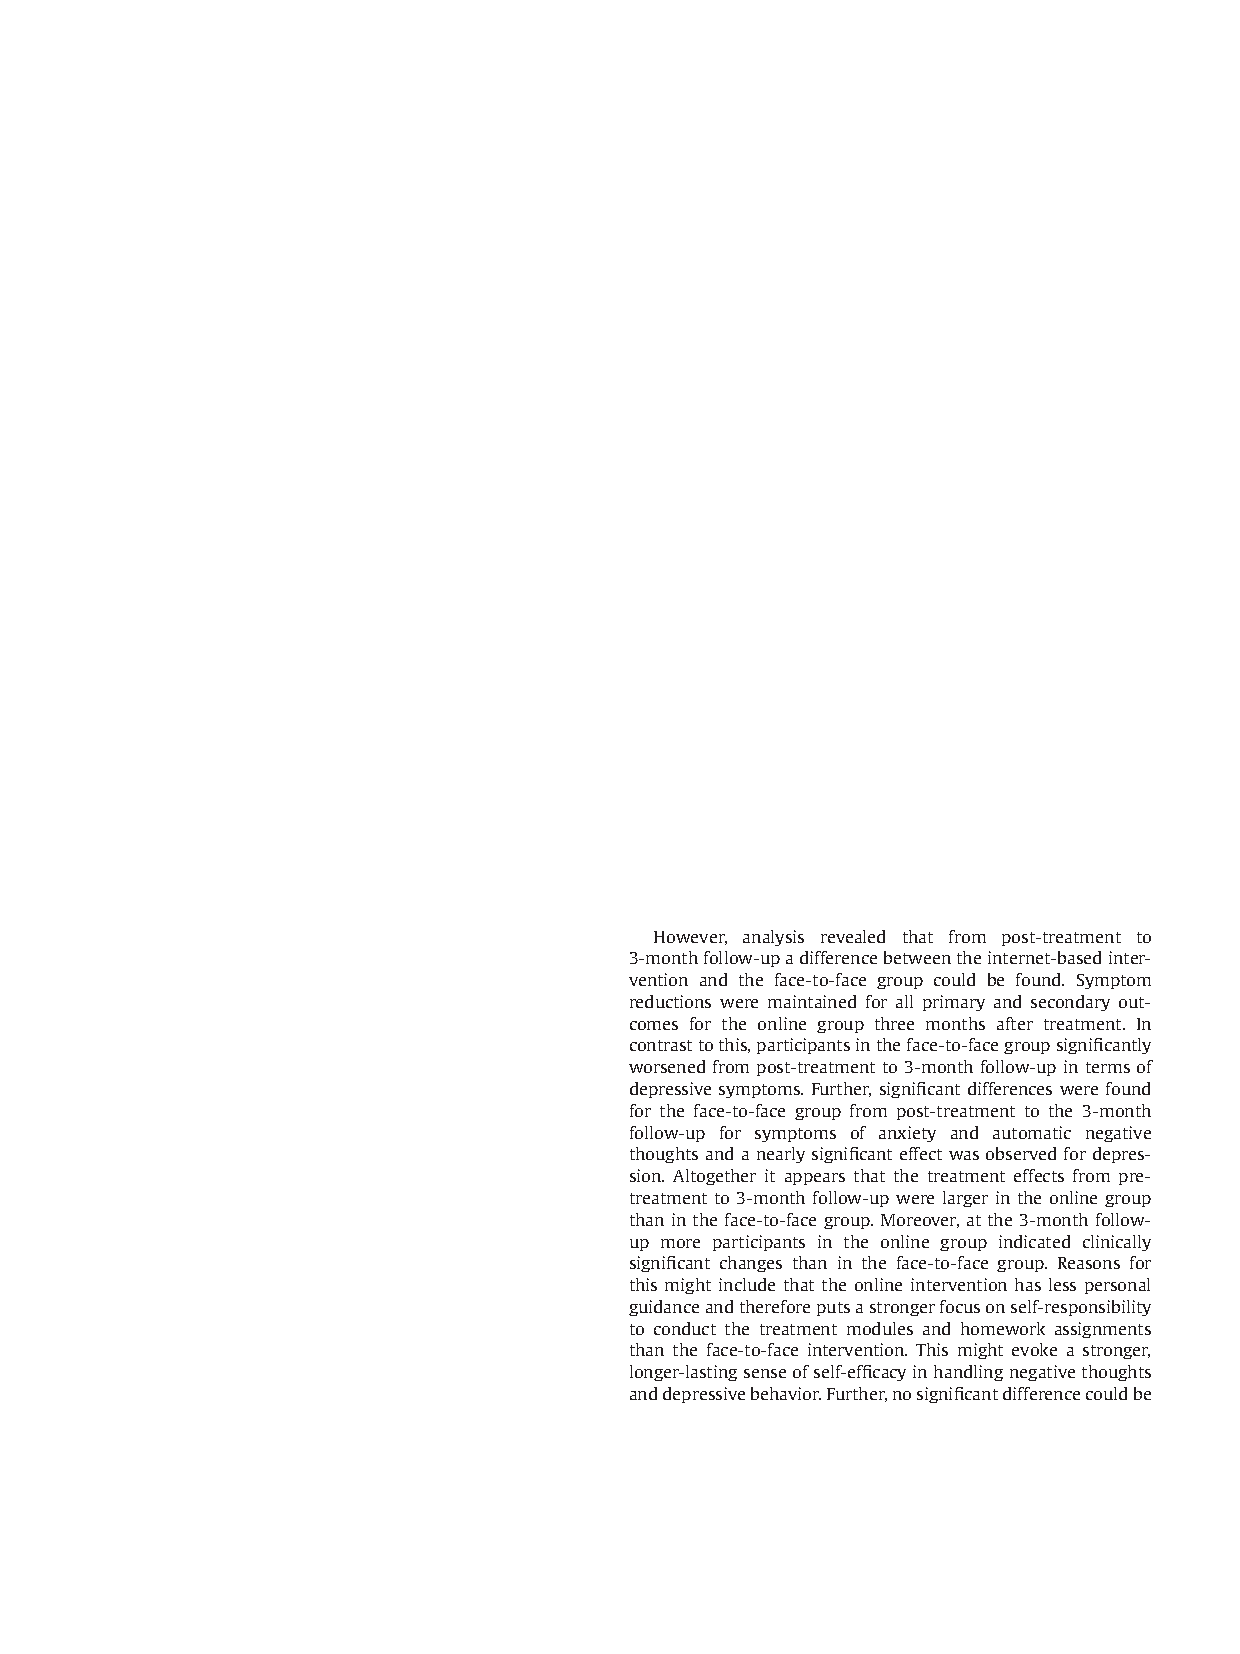
\includegraphics[width=0.5\linewidth]{8_Abbildungen/alm_8_article_discussion} \end{center}
\flushright
\footnotesize

\emph{Wagner, Horn, and Maercker (2014)}
\end{frame}

\begin{frame}[t]{Anwendungskontext}
\protect\hypertarget{anwendungskontext-14}{}
\begin{center}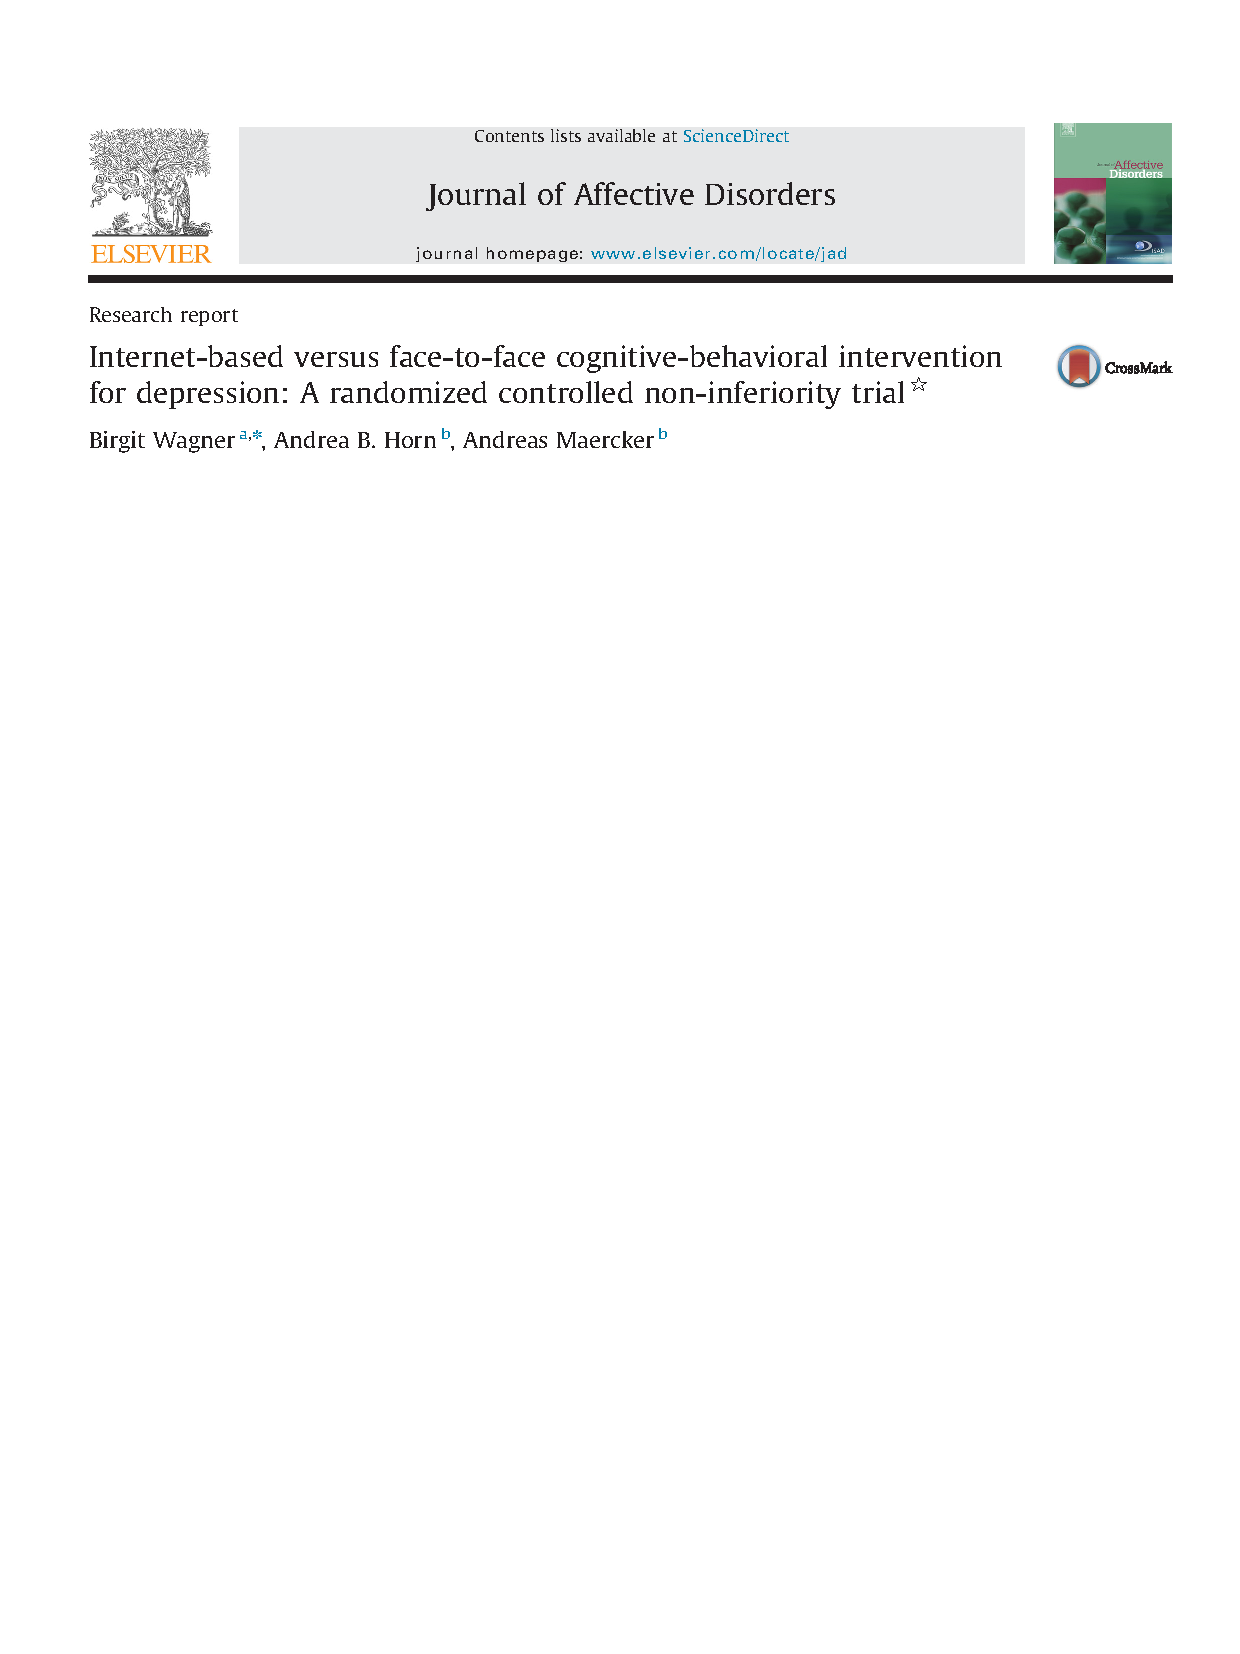
\includegraphics[width=0.5\linewidth]{8_Abbildungen/alm_8_article_title} \end{center}
\center

\textcolor{darkblue}{Conclusion} \vspace{5mm}

\begin{center}
\includegraphics[width=0.5\linewidth]{8_Abbildungen/alm_8_article_conclusion} \end{center}
\vfill
\flushright
\footnotesize

\emph{Wagner, Horn, and Maercker (2014)}
\end{frame}

\begin{frame}[t]{Anwendungskontext}
\protect\hypertarget{anwendungskontext-15}{}
\begin{center}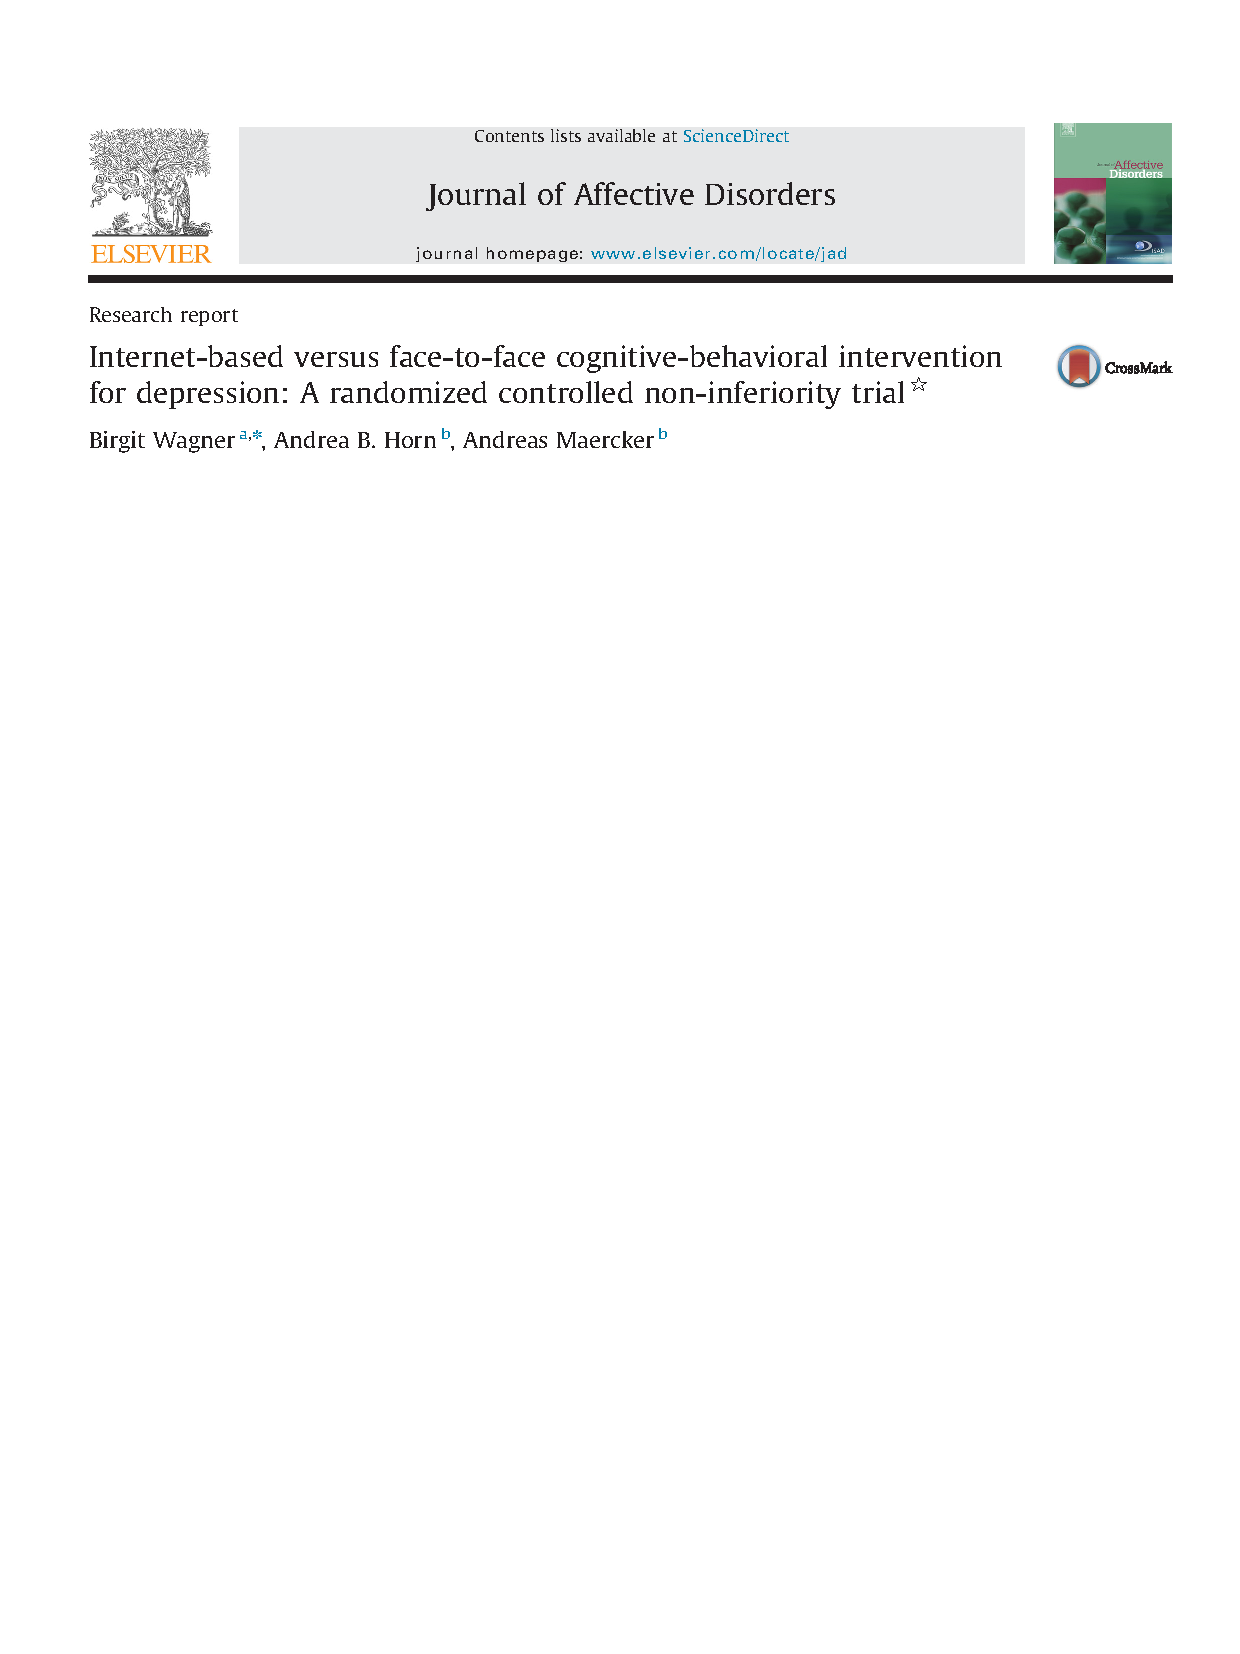
\includegraphics[width=0.5\linewidth]{8_Abbildungen/alm_8_article_title} \end{center}

\begin{center}
\includegraphics[width=0.65\linewidth]{8_Abbildungen/alm_8_article_anzctr} \end{center}
\end{frame}

\begin{frame}[t]{Anwendungskontext}
\protect\hypertarget{anwendungskontext-16}{}
\begin{center}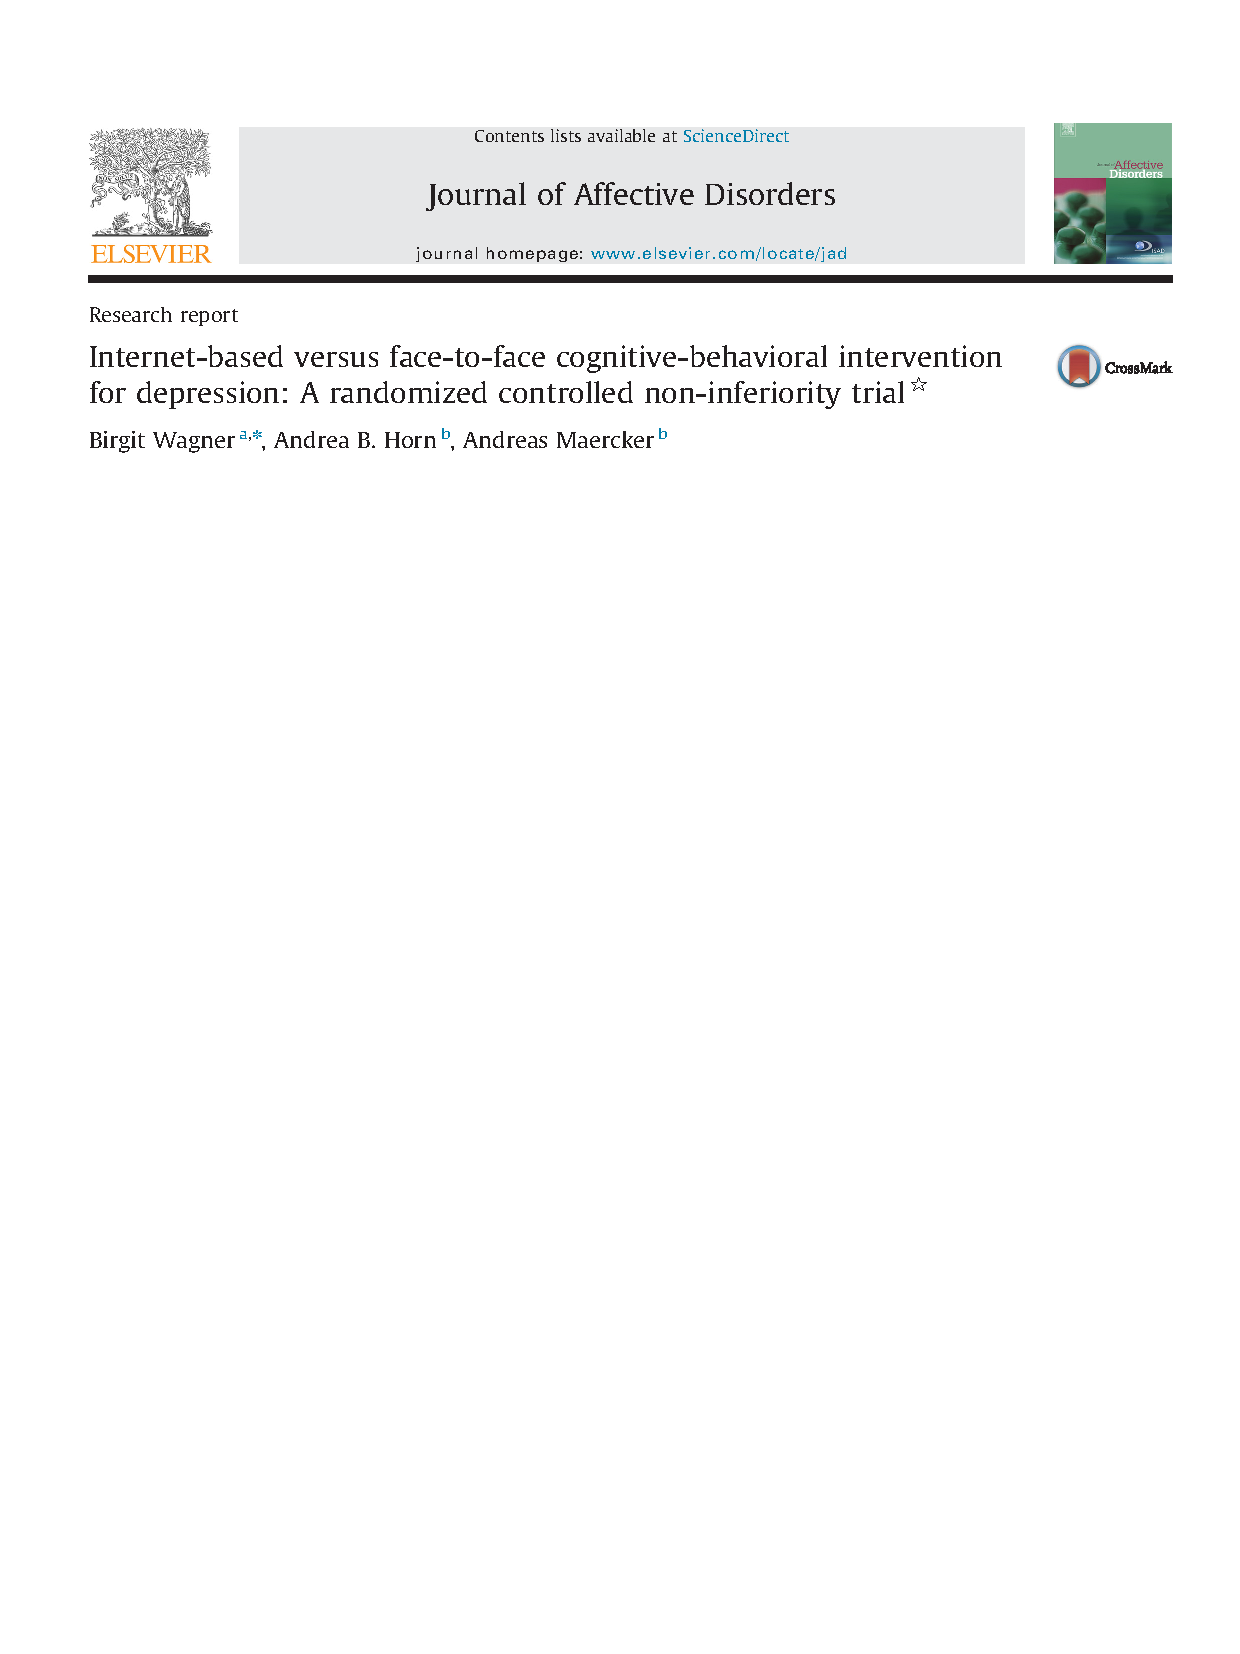
\includegraphics[width=0.5\linewidth]{8_Abbildungen/alm_8_article_title} \end{center}
\vspace{2mm}

\begin{center}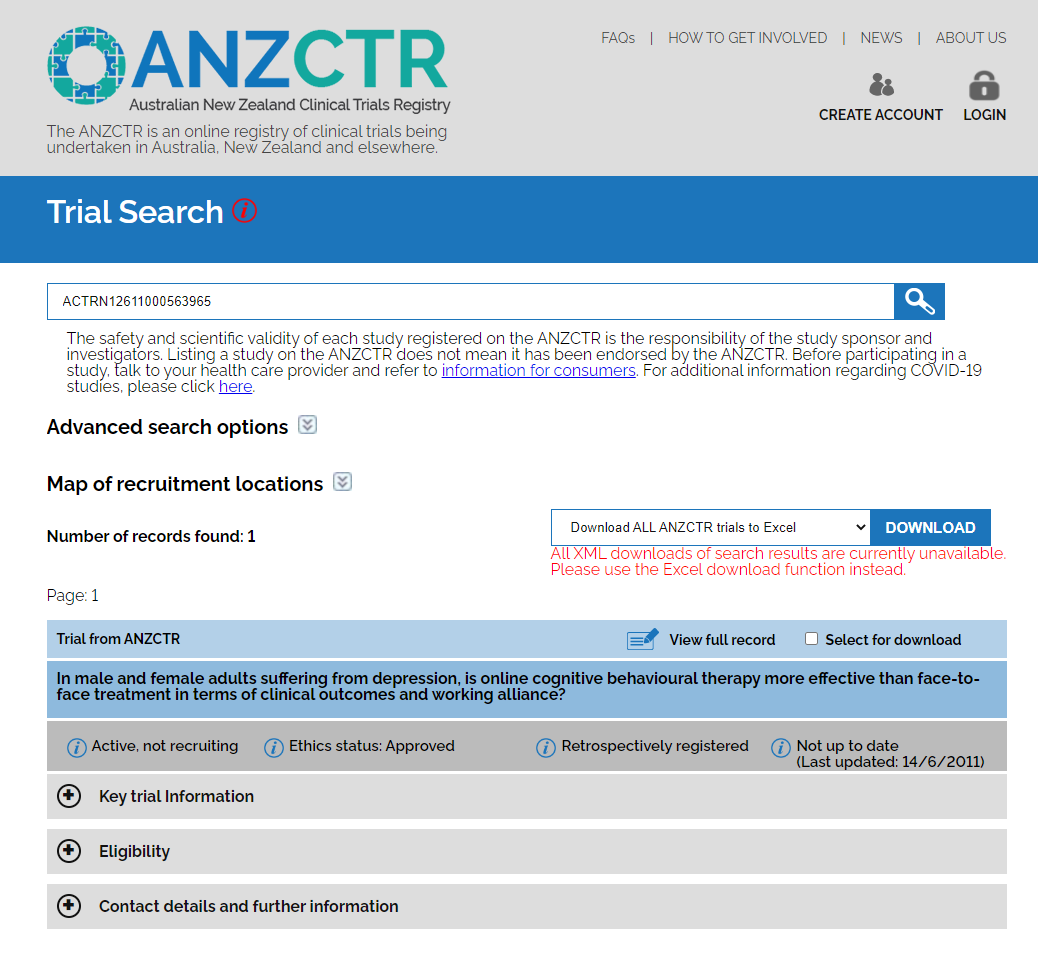
\includegraphics[width=0.5\linewidth]{8_Abbildungen/alm_8_article_registration} \end{center}
\end{frame}

\begin{frame}[t]{Anwendungskontext}
\protect\hypertarget{anwendungskontext-17}{}
\begin{center}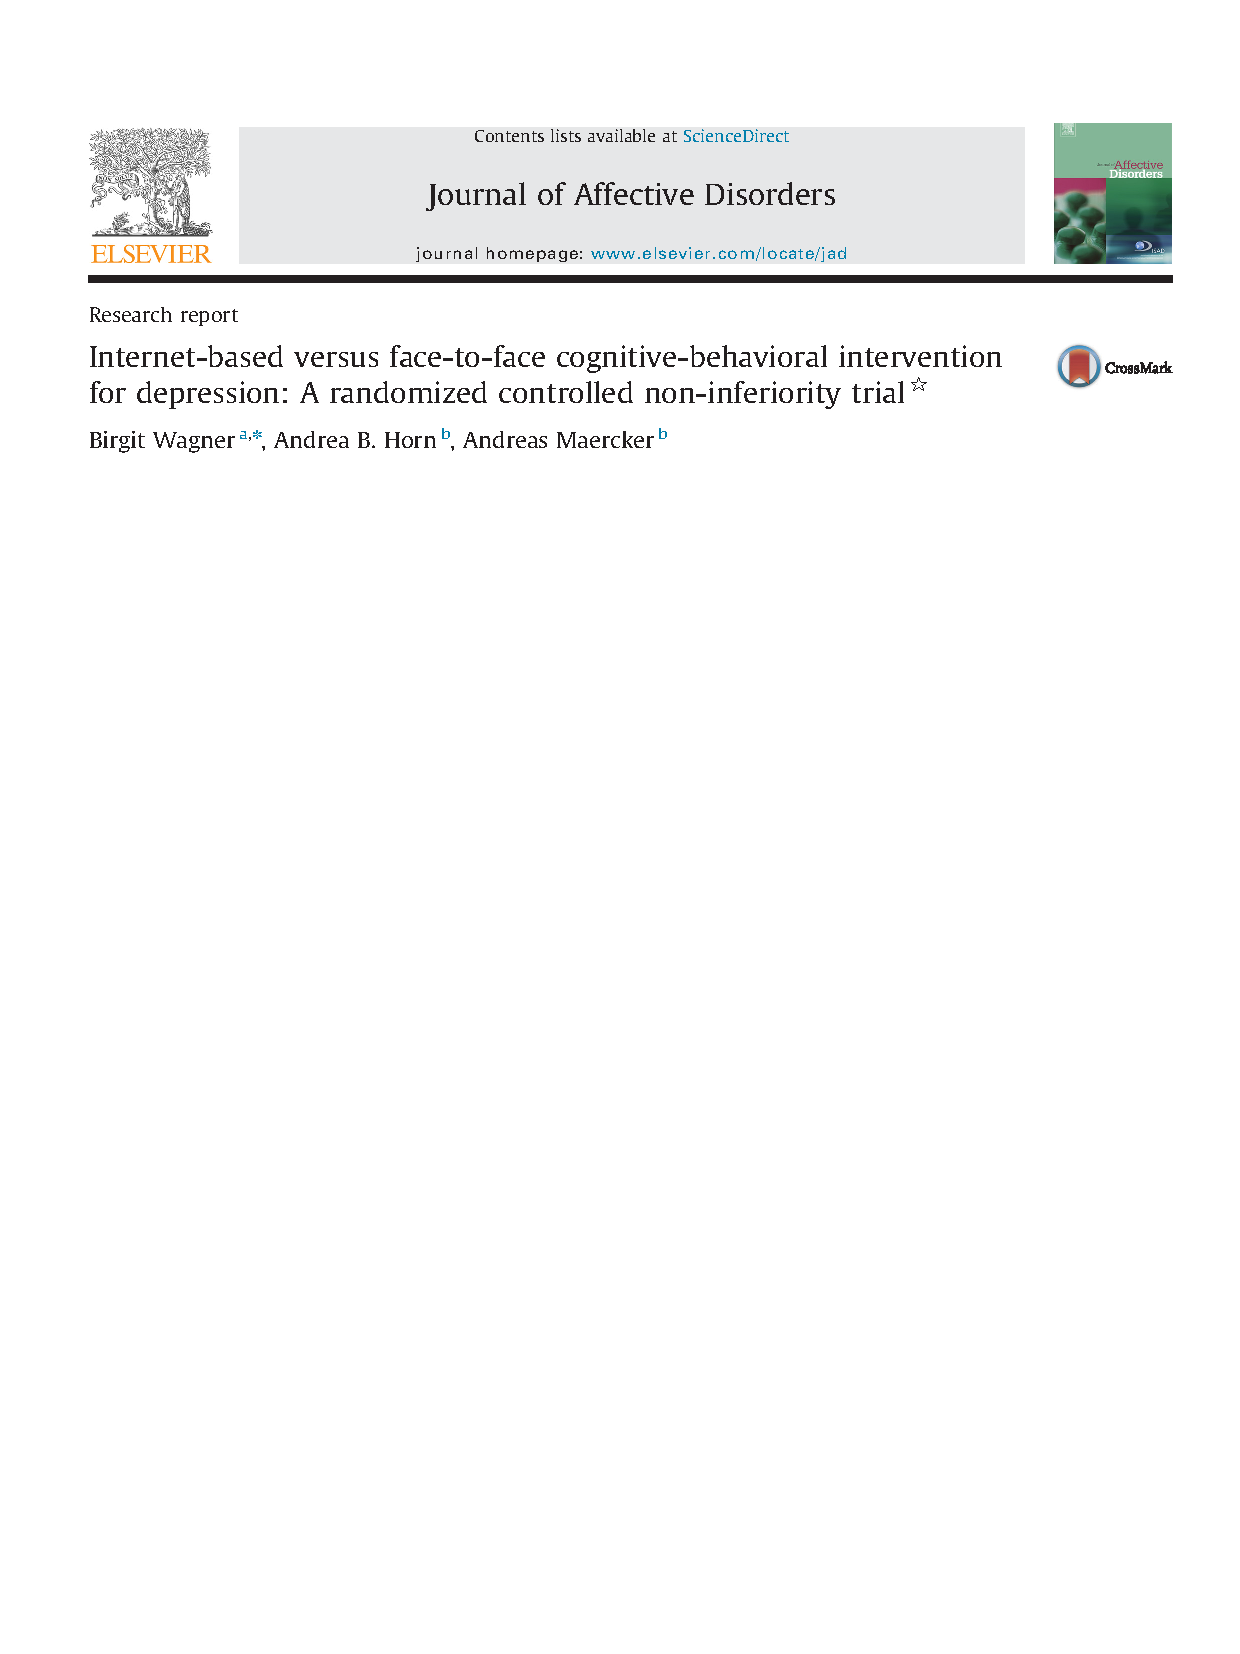
\includegraphics[width=0.5\linewidth]{8_Abbildungen/alm_8_article_title} \end{center}
\vspace{2mm}

\begin{center}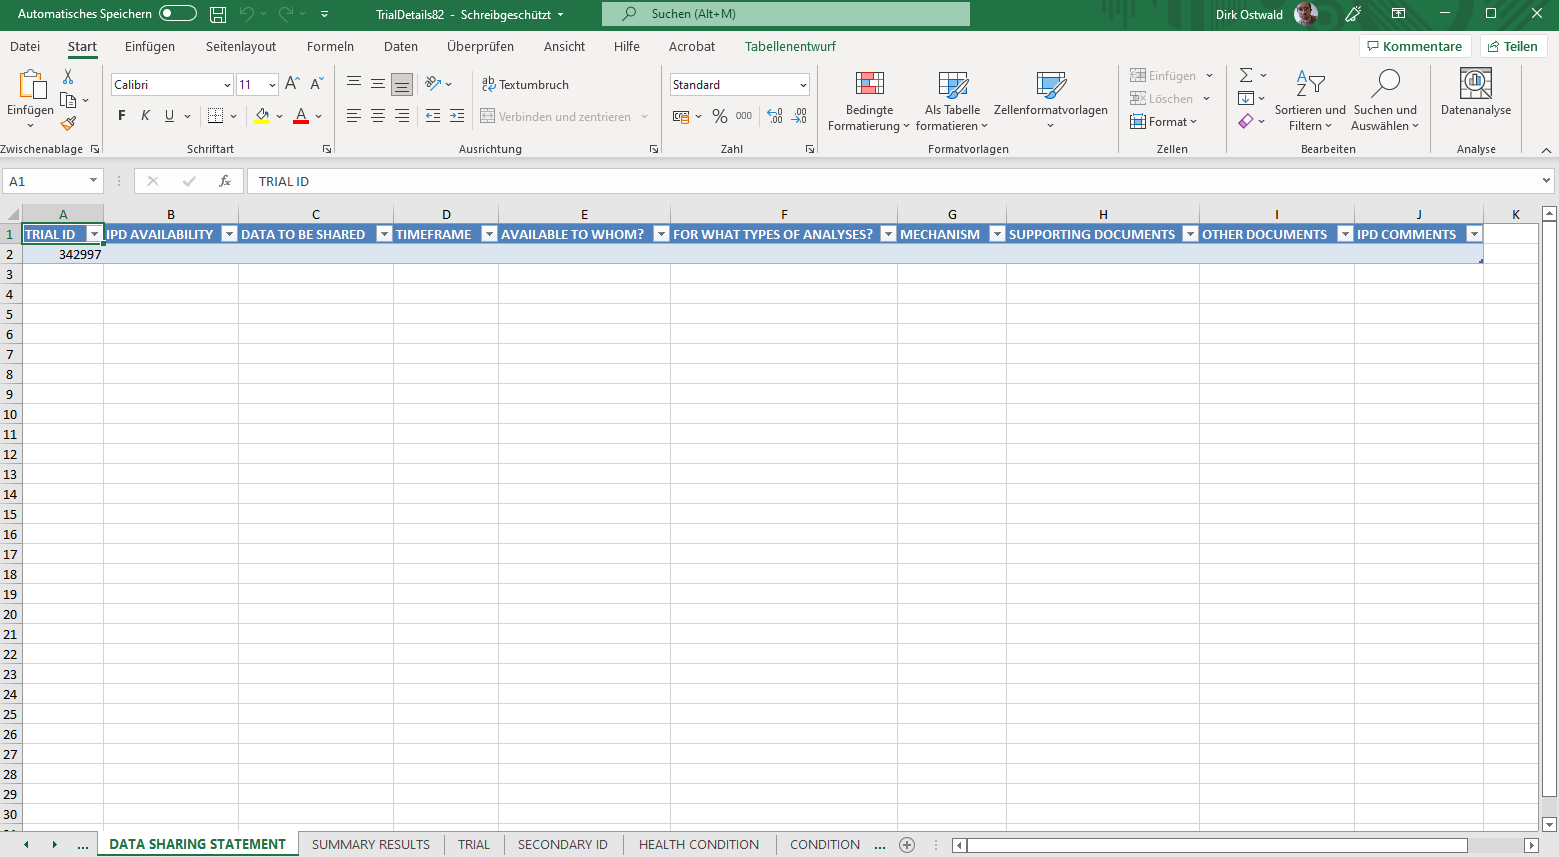
\includegraphics[width=0.8\linewidth]{8_Abbildungen/alm_8_article_data_sharing} \end{center}
\end{frame}

\begin{frame}[plain]{}
\protect\hypertarget{section-7}{}
\vfill
\large
\setstretch{2.5}

Grundbegriffe

Randomisierte einfaktorielle Studiendesigns

Randomisierte mehrfaktorielle Studiendesigns

Anwendungskontext

\textbf{Anwendungsbeispiel}

Selbstkontrollfragen \vfill
\end{frame}

\begin{frame}{Anwendungsbeispiel}
\protect\hypertarget{anwendungsbeispiel}{}
\begin{center}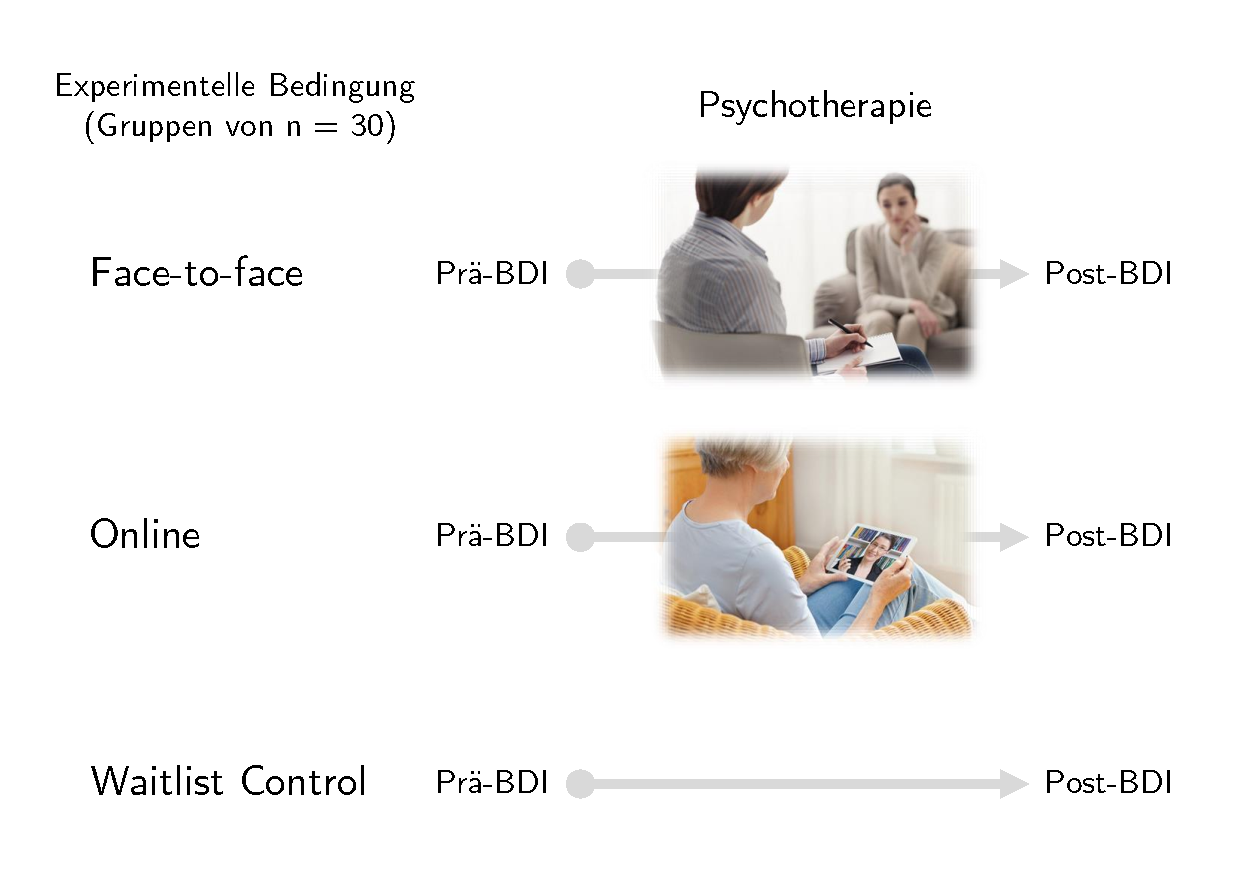
\includegraphics[width=1\linewidth]{8_Abbildungen/alm_8_modellstudie} \end{center}
\end{frame}

\begin{frame}{Anwendungsbeispiel}
\protect\hypertarget{anwendungsbeispiel-1}{}
\normalsize

\textcolor{darkblue}{Experimentelle Einheiten}

\small

Randomisierte Zuordnung von Patient:innen zu den experimentellen Gruppen

\(\bullet\) Unabhängig und identisch verteilte Fehlervariablen

\normalsize

\textcolor{darkblue}{Abhängige Variable}

\small

Negative Post-BDI vs.~Prä-BDI Differenz

\(\bullet\) Univariate abhängige Variable \(\Leftrightarrow\) Ein Wert
pro Patient:in

\(\bullet\) Positive Werte \(\,\,\Leftrightarrow\) Verringerung der
Depressionssymptomatik

\(\bullet\) Negative Werte \(\Leftrightarrow\) Verstärkung der
Depressionssymptomatik

\normalsize

\textcolor{darkblue}{Unabhängige Variablen}

\small

Experimentelle Gruppen \(\Leftrightarrow\) Psychotherapie Setting

\(\bullet\) Face-to-face (F2F), Online (ONL), Waitlist Control (WLC)

Patient:innen Alter in Jahren

Anzahl Therapiestunden
\end{frame}

\begin{frame}[t]{Anwendungsbeispiel}
\protect\hypertarget{anwendungsbeispiel-2}{}
\center

\textcolor{darkblue}{Beispieldatensatz}

\begin{center}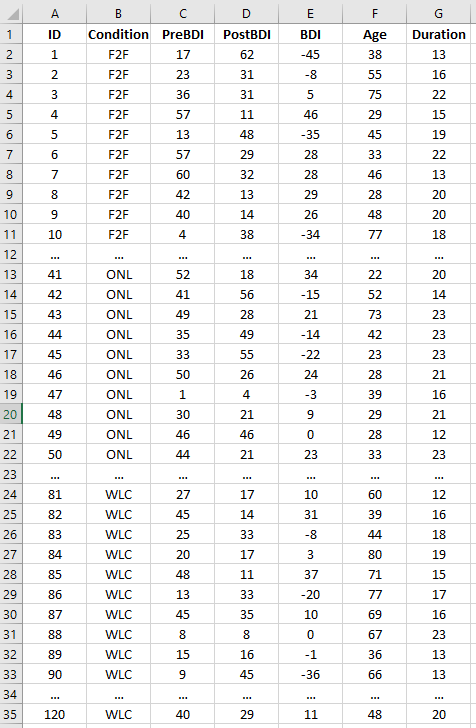
\includegraphics[width=0.4\linewidth]{8_Abbildungen/alm_8_model_datensatz} \end{center}
\end{frame}

\begin{frame}[plain]{}
\protect\hypertarget{section-8}{}
\vfill
\large
\setstretch{2.5}

Grundbegriffe

Randomisierte einfaktorielle Studiendesigns

Randomisierte mehrfaktorielle Studiendesigns

Anwendungskontext

Anwendungsbeispiel

\textbf{Selbstkontrollfragen} \vfill
\end{frame}

\begin{frame}{Selbstkontrollfragen}
\protect\hypertarget{selbstkontrollfragen}{}
\footnotesize
\setstretch{1.6}

\begin{enumerate}
\tightlist
\item
  Erläutern Sie die Begriffe der empirischen Studie, der theoretischen
  Studie, und der Methodenstudie.
\item
  Erläutern Sie die Begriffe der unabhängigen Variable, der abhängigen
  Variable, und der experimentellen Einheit.
\item
  Erläutern Sie die Begriffe der diskreten Variable und der
  kontinuierlichen Variable.
\item
  Erläutern Sie die Begriffe der randomisierten und der
  nicht-randomisierten kontrollierten Studie.
\item
  Erläutern Sie die Begriffe des Quasiexperiments und der
  Korrelationsstudie.
\item
  Nennen Sie drei Charakteristika randomisierter kontrollierter Studien.
\item
  Erläutern Sie die Begriffe des faktoriellen und des parametrischen
  Studiendesigns.
\item
  Erläutern Sie die Begriffe des Between-Group Designs und des
  Within-Group Designs.
\item
  Erläutern Sie die Begriffe des Studiendesigns mit Randomisierung bzw.
  mit Wiederholungsmessung.
\item
  Erläutern Sie den Begriff des randomisierten einfaktoriellen
  Studiendesigns.
\item
  Diskutieren Sie Vor- und Nachteile von No-Treatment und
  Placebo-Treatment Kontrollgruppen.
\item
  Diskutieren Sie Vor- und Nachteile von Zwei-Treatment Vergleichen ohne
  und mit Placebo-Kontrollgruppe.
\item
  Erläutern Sie Vor- und Nachteile von reinen Posttest-Designs und Pre-
  und Posttest Designs.
\item
  Erläutern Sie die Begriffe des mehrfaktoriellen Studiendesigns, des
  Crossed Designs, und des Nested Designs.
\item
  Erläutern Sie den Begriff des randomisierten zweifaktoriellen
  Studiendesigns mit Crossed Design.
\item
  Wieviele Faktoren mit jeweils wie vielen Leveln hat ein 3 x 4 x 2
  Design?
\item
  Wieviele experimentelle Bedingungen hat ein 3 x 4 x 2 Design?
\item
  Erläutern Sie die Begriffe des Haupteffektes und der Interaktion am
  Beispiel eines 2 x 2 Studiendesigns.
\end{enumerate}
\end{frame}

\begin{frame}{References}
\protect\hypertarget{references}{}
\footnotesize

\hypertarget{refs}{}
\begin{CSLReferences}{1}{0}
\leavevmode\hypertarget{ref-moshe_2021}{}%
Moshe, Isaac, Yannik Terhorst, Paula Philippi, Matthias Domhardt, Pim
Cuijpers, Ioana Cristea, Laura Pulkki-Råback, Harald Baumeister, and
Lasse B. Sander. 2021. {``Digital Interventions for the Treatment of
Depression: {A} Meta-Analytic Review.''} \emph{Psychological Bulletin}
147 (8): 749--86. \url{https://doi.org/10.1037/bul0000334}.

\leavevmode\hypertarget{ref-wagner_2014}{}%
Wagner, Birgit, Andrea B. Horn, and Andreas Maercker. 2014.
{``Internet-Based Versus Face-to-Face Cognitive-Behavioral Intervention
for Depression: {A} Randomized Controlled Non-Inferiority Trial.''}
\emph{Journal of Affective Disorders} 152--154 (January): 113--21.
\url{https://doi.org/10.1016/j.jad.2013.06.032}.

\end{CSLReferences}
\end{frame}

\end{document}
